% =============================================================================
%  Two-Timescale Secure Transmission for MA-Enabled Multiuser Systems
%  With Statistical Eavesdropper CSI
%  Compile with pdfLaTeX and the official IEEEtran.cls (TeX Live / Overleaf).
% =============================================================================
\documentclass[journal]{IEEEtran}
\usepackage{amsmath,amssymb,amsfonts}
\interdisplaylinepenalty=2500
\usepackage{algorithm}
\usepackage{algpseudocode}
\renewcommand{\algorithmicrequire}{\textbf{Input:}}
\renewcommand{\algorithmicensure}{\textbf{Output:}}
\usepackage{cite}
\usepackage{graphicx}
\usepackage[caption=false,font=footnotesize]{subfig}
% Figures redrawn from the completed, independently checked simulation arrays.
\graphicspath{{ma_secrecy_matlab/figures_revised_regenerated/}}
\usepackage{tikz}
\usetikzlibrary{arrows.meta,decorations.pathreplacing,calc,shapes.symbols}
\definecolor{fblue}{HTML}{2E6DB4}
\definecolor{fred}{HTML}{B03A2E}
\definecolor{fteal}{HTML}{2A9D8F}
\definecolor{fochre}{HTML}{C7852B}
\newcommand{\phoneicon}[2]{% handset icon at #1 with screen color #2 (Fig. 1)
  \begin{scope}[shift={#1}]
    \draw[rounded corners=1.3pt, line width=0.5pt, fill=white] (-0.135,-0.25) rectangle (0.135,0.25);
    \fill[#2] (-0.1,-0.17) rectangle (0.1,0.2);
    \fill[black!55] (0,-0.212) circle (0.02);
  \end{scope}}

% ------------------------------- theorem-like --------------------------------
\newtheorem{lemma}{Lemma}
\newtheorem{proposition}{Proposition}
\newtheorem{remark}{Remark}

% ----------------------------- notation macros -------------------------------
\newcommand{\E}{\mathbb{E}}
\newcommand{\CN}{\mathcal{CN}}
\newcommand{\tr}{\operatorname{Tr}}
\newcommand{\diag}{\operatorname{diag}}
\newcommand{\RE}{\operatorname{Re}}
\newcommand{\bt}{\mathbf{t}}
\newcommand{\bh}{\mathbf{h}}
\newcommand{\bg}{\mathbf{g}}
\newcommand{\hb}{\bar{\mathbf{h}}}
\newcommand{\gb}{\bar{\mathbf{g}}}
\newcommand{\htl}{\tilde{\mathbf{h}}}
\newcommand{\gtl}{\tilde{\mathbf{g}}}
\newcommand{\bH}{\mathbf{H}}
\newcommand{\Hb}{\bar{\mathbf{H}}}
\newcommand{\Htl}{\tilde{\mathbf{H}}}
\newcommand{\bK}{\mathbf{K}}
\newcommand{\bB}{\mathbf{B}}
\newcommand{\bL}{\mathbf{L}}
\newcommand{\bI}{\mathbf{I}}
\newcommand{\bw}{\mathbf{w}}
\newcommand{\wb}{\bar{\mathbf{w}}}
\newcommand{\bv}{\mathbf{v}}
\newcommand{\bp}{\mathbf{p}}
\newcommand{\ba}{\mathbf{a}}
\newcommand{\be}{\mathbf{e}}
\newcommand{\bb}{\mathbf{b}}
\newcommand{\bl}{\mathbf{l}}
\newcommand{\br}{\mathbf{r}}
\newcommand{\bx}{\mathbf{x}}
\newcommand{\bz}{\mathbf{z}}
\newcommand{\bF}{\mathbf{F}}
\newcommand{\Fb}{\bar{\mathbf{F}}}
\newcommand{\bW}{\mathbf{W}}
\newcommand{\bD}{\mathbf{D}}
\newcommand{\bX}{\mathbf{X}}
\newcommand{\bOm}{\boldsymbol{\Omega}}
\newcommand{\bPhi}{\boldsymbol{\Phi}}
\newcommand{\bGam}{\boldsymbol{\Gamma}}
\newcommand{\bSig}{\boldsymbol{\Sigma}}
\newcommand{\bDel}{\boldsymbol{\delta}}
\newcommand{\bPi}{\boldsymbol{\Pi}}
\newcommand{\Ptot}{P_{\mathrm{tot}}}
\newcommand{\Dmin}{D_{\mathrm{min}}}
\newcommand{\sbe}{\bar{\sigma}_{\mathrm{e}}^2}
\newcommand{\PHp}{\mathbf{P}^{\perp}(\bt)}


\begin{document}

\title{Two-Timescale Secure Transmission for Movable Antenna-Enabled Multiuser Systems With Statistical Eavesdropper CSI}

\author{Author~One,~\IEEEmembership{Student Member,~IEEE,}
        Author~Two,~\IEEEmembership{Member,~IEEE}
\thanks{The authors are with ... (e-mail: ...).}}

\markboth{IEEE Transactions on Communications (draft)}{}

\maketitle

\begin{abstract}
Movable antenna (MA) arrays can separate nearly aligned legitimate and eavesdropping channels, but repositioning under fast fading incurs mechanical overhead. We formulate ergodic secrecy sum rate (ESSR) maximization by jointly optimizing antenna positions and long-term information and artificial noise (AN) powers under total-power, movement-region, and minimum-spacing constraints, using statistical channel state information (CSI). We restrict the instantaneous transmission policy to zero-forcing (ZF) precoding and null-space AN based on legitimate-channel CSI. The resulting problem couples random beamforming directions and AN subspaces with nonconcave position-dependent rates and nonconvex spacing constraints. To obtain a deterministic design objective, we derive conditional leakage and AN moments from their orthogonal Gaussian channel components and construct closed-form moment approximations; these approximations are not secrecy-rate bounds. For fixed positions and AN power, user screening yields a concave power-allocation problem with a secrecy water-filling solution, while a finite coarse-to-fine search selects the AN power. For fixed powers, a feasible grid search identifies position candidates, and quadratic minorization with linearized spacing constraints reduces local refinement to projection onto a convex polygon. Alternating these updates produces a nondecreasing, bounded surrogate-objective sequence without sampling channel realizations during optimization; Monte Carlo evaluation at a transmit signal-to-noise ratio of 20~dB gives a 14.8\% ESSR gain over the rate-oriented two-timescale MA benchmark in the default setting.
\end{abstract}

\begin{IEEEkeywords}
Movable antenna, physical layer security, artificial noise, two-timescale design, statistical CSI, ergodic secrecy rate.
\end{IEEEkeywords}

\IEEEpeerreviewmaketitle

% =============================================================================
\section{Introduction}\label{sec:intro}
% =============================================================================
\IEEEPARstart{P}{hysical} layer security exploits wireless channel randomness and spatial selectivity to protect confidential messages, complementing upper-layer cryptography~\cite{Wyner1975,Mukherjee2014,WuJSAC2018}. In multi-antenna systems, secure precoding directs confidential signals toward legitimate users (LUs), while artificial noise (AN) introduces interference at an eavesdropper (Eve)~\cite{Goel2008,Zhou2010}. Both techniques depend on spatial separation between the LUs and Eve~\cite{Mukherjee2014}. When Eve and an LU have similar departure angles and line-of-sight (LoS) propagation dominates, their channels are strongly correlated. A fixed-position antenna (FPA) array then has limited ability to suppress leakage without reducing the desired-signal gain.

Movable antennas (MAs)~\cite{ZhuMag2024,ZhuTWC2024Model} and fluid antennas~\cite{WongTWC2021} adjust antenna positions within a prescribed region. This additional spatial freedom changes the channel correlations among receivers without increasing the number of radio-frequency (RF) chains~\cite{MaTWC2024,ZhuTWC2024MU,ZhuCL2023}. The secure design in~\cite{HuSPL2024} jointly optimizes transmit beamforming and antenna positions with perfect channel state information (CSI), while~\cite{HuTMC2024} considers unavailable instantaneous eavesdropper CSI. The analysis in~\cite{XieArxiv2026} derives a deterministic equivalent of the ergodic secrecy rate for a multiple-input multiple-output MA system with statistical CSI of a multi-antenna Eve. The sensing-assisted design in~\cite{ChenArxiv2026} optimizes positions to improve the estimation of Eve's angles of departure (AoDs) and the secrecy rate.

The designs in~\cite{HuSPL2024,HuTMC2024,XieArxiv2026} use instantaneous legitimate-channel CSI for position optimization. Tracking these designs under fast fading requires position adaptation on the channel coherence interval (CI), with associated movement delay and energy consumption. Acquiring channel information over the movable region also requires measurements at multiple antenna positions~\cite{ZhengTCOM2025,HuTVT2025}. The LoS model in~\cite{ChenArxiv2026} does not characterize the effect of small-scale fading on long-term secrecy.

Two-timescale designs reduce position-adaptation and CSI-acquisition overhead by separating slow statistical optimization from fast precoding. This approach is studied for intelligent reflecting surfaces in~\cite{ZhaoTWC2021} and for MA systems in~\cite{ZhengTCOM2025,HuTVT2025}. The antenna positions depend on statistical CSI, whereas the precoders depend on the instantaneous effective channels at those positions. The downlink design in~\cite{ZhengTCOM2025} maximizes the ergodic sum rate with maximum-ratio transmission or zero-forcing (ZF) precoding, and the uplink design in~\cite{HuTVT2025} considers linear and successive interference cancellation receivers. These rate objectives do not include information leakage to Eve.

A secrecy objective introduces three coupled requirements. First, Eve's ergodic wiretap rate depends on the random ZF directions and AN subspace induced by the LU channels; intended-user rate approximations~\cite{ZhangJSTSP2014,ZhengTCOM2025,HuTVT2025} do not determine this leakage. Second, position optimization must characterize both the confidential signal and the AN received by Eve. These effects remain relevant with one LU, for which the rate-oriented position design provides no gain under the adopted channel model~\cite[Remark~2]{ZhengTCOM2025}. Third, changing the positions changes the effective LU gains, leakage gains, and AN gain at Eve, which in turn changes the allocation of power between confidential signals and AN.

The remaining design task is to optimize long-term antenna positions and powers when the wiretap rate depends on the instantaneous ZF directions and AN subspace of the legitimate channels. A rate-oriented position design addresses interference among the LUs, but does not directly control leakage to Eve or its received AN power. We therefore formulate joint ergodic secrecy sum rate (ESSR) maximization with statistical CSI of the LUs and Eve, restrict the short-timescale policy to ZF precoding and isotropic null-space AN, and construct a deterministic approximate objective for the long-term variables. This restriction preserves per-realization power feasibility but does not solve the unrestricted precoding-policy problem. The principal contributions are as follows.
\begin{enumerate}
\item \textit{Wiretap-rate approximation and spatial mechanisms:} Under independent, spatially isotropic Gaussian non-line-of-sight (NLoS) components, we prove conditional independence between the information leakage and the AN-channel energy given the LU channels. We then approximate the random channel moments and the ergodic wiretap rate in closed form. The resulting coefficients characterize leakage along the ZF directions and AN coupling to Eve, in addition to the LU correlation that determines the ZF gain. These approximations are design surrogates rather than certified secrecy-rate bounds; their accuracy is evaluated by Monte Carlo simulation.
\item \textit{Power-allocation decomposition:} For fixed positions and AN power, we identify the users whose legitimate effective gains exceed Eve's gains. The remaining power-allocation problem is strictly concave and admits a secrecy water-filling solution with one dual variable, obtained by bisection. We evaluate the resulting value function over finite coarse and refined AN-power grids because its unimodality is not established. This procedure provides a feasible candidate and does not certify a continuous global optimum.
\item \textit{Feasible position updates and objective convergence:} We develop an alternating optimization (AO) algorithm. For fixed powers, a rank-one Gram-matrix representation permits efficient evaluation of each antenna's feasible grid candidates. Majorization--minimization (MM) refinement uses a quadratic lower model and an inner linear approximation of the spacing constraints, reducing the local update to projection onto a convex polygon. Retaining the current position and accepting only nondecreasing power updates yield a bounded, nondecreasing surrogate-objective sequence. The convergence statement concerns objective values; joint stationarity and global optimality are not established.
\item \textit{Evaluation with the original channel model:} Designs computed from the approximations are evaluated using the instantaneous signal-to-interference-plus-noise ratios (SINRs) over independently generated small-scale fading realizations. In the default setting at a transmit signal-to-noise ratio (SNR) of $20$~dB, the proposed design achieves $20.75$~bps/Hz, compared with $18.08$~bps/Hz for the rate-oriented MA benchmark~\cite{ZhengTCOM2025}, a gain of $14.8\%$. Comparisons with antenna selection (AS) and fixed arrays also examine the AN fraction and antenna count, while additional tests consider single-user operation and errors in Eve's statistical CSI. All reported comparisons refer to the tested channel and resource settings.
\end{enumerate}

\textit{Notation:} Scalars, vectors, and matrices are denoted by italic, bold lowercase, and bold uppercase letters, respectively; sets are denoted by calligraphic letters. The spaces of $a\times b$ complex and real matrices are $\mathbb{C}^{a\times b}$ and $\mathbb{R}^{a\times b}$. The operators $(\cdot)^{\mathrm{T}}$, $(\cdot)^{\mathrm{*}}$, and $(\cdot)^{\mathrm{H}}$ denote transpose, conjugation, and conjugate transpose, respectively. The symbols $|\cdot|$, $\|\cdot\|$, and $\tr(\cdot)$ denote modulus, Euclidean norm, and trace. Vector and matrix entries are written as $[\mathbf{x}]_i$ and $[\bX]_{i,j}$. The diagonal entries of $\diag(x_1,\ldots,x_M)$ are $x_1,\ldots,x_M$. For a nonnegative diagonal matrix $\bX$, $\bX^{1/2}$ denotes its entrywise square root. The matrix $\bI_N$ is the $N\times N$ identity matrix, and $\be_m$ is the $m$th standard basis vector of the required dimension. The notation $\CN(\boldsymbol{\mu},\bSig)$ denotes a proper complex Gaussian distribution with mean $\boldsymbol{\mu}$, covariance $\bSig$, and zero pseudocovariance. Positive semidefiniteness and positive definiteness are written as $\bX\succeq\mathbf{0}$ and $\bX\succ\mathbf{0}$. We use $j\triangleq\sqrt{-1}$, $\E\{\cdot\}$ for expectation, $\mathrm{Var}\{\cdot\}$ for variance, $\RE\{\cdot\}$ for the real part, and $\nabla_{\mathbf{x}}f$ for the gradient with respect to $\mathbf{x}$. Finally, $[x]^+\triangleq\max\{x,0\}$, $\lfloor x\rfloor$ is the largest integer not exceeding $x$, $|\mathcal{S}|$ is the cardinality of $\mathcal{S}$, and $\mathcal{O}(\cdot)$ and $o(\cdot)$ denote big-O and little-o order, respectively.

% =============================================================================
\section{System Model and Problem Formulation}\label{sec:model}
% =============================================================================

\subsection{MA-Enabled Secure Multiuser Downlink System}

\begin{figure}[t]
\centering
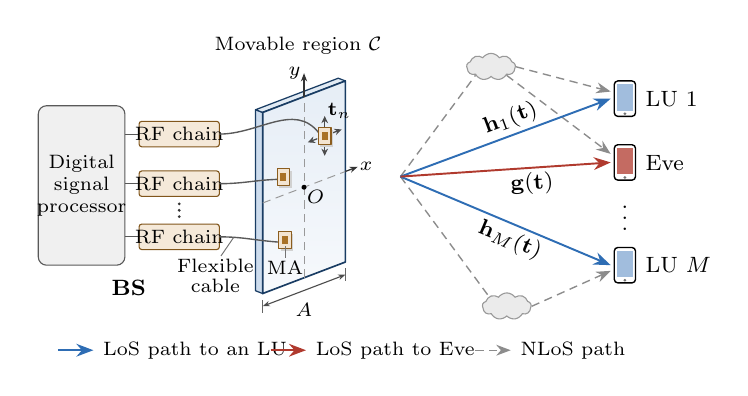
\begin{tikzpicture}[font=\footnotesize, >=Stealth, x=1cm, y=0.9cm]
  % BS: digital signal processor and RF chains
  \draw[rounded corners=3pt, fill=black!6, draw=black!65] (0,1.2) rectangle (1.1,3.45);
  \node[align=center, font=\scriptsize] at (0.55,2.32) {Digital\\signal\\processor};
  \foreach \y in {3.05, 2.35, 1.6}{
    \draw[black!65] (1.1,\y) -- (1.28,\y);
    \draw[rounded corners=1pt, fill=fochre!18, draw=fochre!65!black] (1.28,\y-0.18) rectangle (2.3,\y+0.18);
    \node[font=\scriptsize] at (1.79,\y) {RF chain};}
  \foreach \d in {-0.09,0,0.09} \fill[black!80] (1.79,1.975+\d) circle (0.55pt);
  \node[font=\footnotesize\bfseries] at (1.15,0.88) {BS};
  % movable region C: a thin board in an oblique view (local frame: C is the unit square)
  \begin{scope}[shift={(2.85,0.8)}, x={(1.05cm,0.4cm)}, y={(0cm,2.3cm)}, line join=round]
    \filldraw[fill=fblue!24, draw=fblue!55!black, line width=0.45pt] (0,0) -- (0,1) -- (-0.086,1.03) -- (-0.086,0.03) -- cycle;
    \filldraw[fill=fblue!14, draw=fblue!55!black, line width=0.45pt] (0,1) -- (1,1) -- (0.914,1.03) -- (-0.086,1.03) -- cycle;
    \shade[bottom color=fblue!4, top color=fblue!12] (0,0) -- (1,0) -- (1,1) -- (0,1) -- cycle;
    \draw[fblue!55!black, line width=0.6pt] (0,0) -- (1,0) -- (1,1) -- (0,1) -- cycle;
    % local coordinate system with the origin O at the center of C
    \draw[black!40, densely dashed, line width=0.35pt] (0.5,0) -- (0.5,1);
    \draw[black!40, densely dashed, line width=0.35pt] (0,0.5) -- (1,0.5);
    \draw[-{Stealth[length=3pt]}, black!80, line width=0.45pt] (1,0.5) -- (1.15,0.5) node[right, inner sep=0.5pt, font=\scriptsize, text=black] {$x$};
    \draw[-{Stealth[length=3pt]}, black!80, line width=0.45pt] (0.5,1) -- (0.5,1.13) node[left, inner sep=1pt, font=\scriptsize, text=black] {$y$};
    \fill[black] (0.5,0.5) circle (0.9pt) node[below right, inner sep=0.8pt, font=\scriptsize] {$O$};
    % cable ends of the MAs (the patches are drawn after the cables)
    \coordinate (P1w) at (0.675,0.772); \coordinate (P2w) at (0.175,0.60); \coordinate (P3w) at (0.195,0.25);
  \end{scope}
  % flexible cables
  \draw[black!65, line width=0.5pt] (2.3,3.05) .. controls (2.8,3.05) and (3.25,3.5) .. (P1w);
  \draw[black!65, line width=0.5pt] (2.3,2.35) .. controls (2.6,2.35) and (2.75,2.4) .. (P2w);
  \draw[black!65, line width=0.5pt] (2.3,1.6) .. controls (2.6,1.6) and (2.75,1.55) .. (P3w);
  \begin{scope}[shift={(2.85,0.8)}, x={(1.05cm,0.4cm)}, y={(0cm,2.3cm)}, line join=round]
    % two-dimensional movement of MA n
    \begin{scope}[black!70, line width=0.45pt, -{Stealth[length=2.6pt, width=2.4pt]}]
      \draw (0.84,0.74) -- (0.955,0.74);  \draw (0.66,0.74) -- (0.545,0.74);
      \draw (0.75,0.78) -- (0.75,0.85);   \draw (0.75,0.70) -- (0.75,0.63);
    \end{scope}
    % MA patches (substrate, radiating patch, and a light shadow)
    \foreach \u/\v in {0.75/0.74, 0.25/0.60, 0.27/0.25}{
      \fill[black!18] (\u-0.051,\v-0.051) rectangle (\u+0.099,\v+0.017);
      \filldraw[fill=fochre!22, draw=fochre!70!black, line width=0.45pt] (\u-0.075,\v-0.034) rectangle (\u+0.075,\v+0.034);
      \fill[fochre!85!black] (\u-0.036,\v-0.016) rectangle (\u+0.036,\v+0.016);}
    \node[font=\scriptsize, inner sep=1pt] at (0.93,0.845) {$\mathbf t_n$};
    % component labels
    \draw[black!55, line width=0.35pt] (0.27,0.214) -- (0.27,0.15);
    \node[below, font=\scriptsize, inner sep=1pt] at (0.27,0.15) {MA};
    % side length
    \draw[black!60, line width=0.35pt] (0,-0.035) -- (0,-0.105) (1,-0.035) -- (1,-0.105);
    \draw[{Stealth[length=2.6pt]}-{Stealth[length=2.6pt]}, black!70, line width=0.4pt] (0,-0.07) -- (1,-0.07) node[midway, below=1pt, font=\scriptsize, text=black] {$A$};
  \end{scope}
  \node[font=\scriptsize] at (3.3,4.3) {Movable region $\mathcal C$};
  \draw[black!55, line width=0.35pt] (2.48,1.59) -- (2.32,1.33);
  \node[align=center, font=\scriptsize, inner sep=1pt, below] at (2.25,1.33) {Flexible\\[-1pt]cable};
  % LoS and NLoS paths to the LUs and Eve
  \tikzset{scat/.style={cloud, cloud puffs=9, cloud puff arc=110, aspect=1.9, draw=black!40, fill=black!8,
             minimum width=0.62cm, minimum height=0.34cm, inner sep=0pt},
           nlos/.style={black!45, densely dashed, line width=0.5pt}, los/.style={->, line width=0.7pt}}
  \coordinate (O) at (4.6,2.45);
  \coordinate (U1) at (7.45,3.55); \coordinate (E) at (7.45,2.65); \coordinate (UM) at (7.45,1.2);
  \node[scat] (S1) at (5.75,4.0) {};
  \node[scat] (S2) at (5.95,0.62) {};
  \draw[nlos] (O) -- (S1.south west);
  \draw[nlos, ->] (S1.east) -- ($(U1)+(-0.18,0.1)$);
  \draw[nlos, ->] (S1.south east) -- ($(E)+(-0.18,0.12)$);
  \draw[nlos] (O) -- (S2.north west);
  \draw[nlos, ->] (S2.east) -- ($(UM)+(-0.18,-0.08)$);
  \draw[los, fblue] (O) -- ($(U1)+(-0.18,0)$) node[pos=0.55, above, sloped, inner sep=1.5pt, text=black] {$\mathbf h_1(\mathbf t)$};
  \draw[los, fblue] (O) -- ($(UM)+(-0.18,0)$) node[pos=0.55, below, sloped, inner sep=1.5pt, text=black] {$\mathbf h_M(\mathbf t)$};
  \draw[los, fred] (O) -- ($(E)+(-0.18,0)$) node[pos=0.62, below, sloped, inner sep=1.5pt, text=black] {$\mathbf g(\mathbf t)$};
  \phoneicon{(U1)}{fblue!45}  \node[right=4pt] at (U1) {LU $1$};
  \phoneicon{(E)}{fred!75}   \node[right=4pt] at (E) {Eve};
  \node at (7.45,1.98) {$\vdots$};
  \phoneicon{(UM)}{fblue!45}  \node[right=4pt] at (UM) {LU $M$};
  % legend
  \begin{scope}[shift={(0.25,0.0)}, font=\scriptsize]
    \draw[los, fblue] (0,0) -- (0.45,0);    \node[right] at (0.45,0) {LoS path to an LU};
    \draw[los, fred] (2.7,0) -- (3.15,0);  \node[right] at (3.15,0) {LoS path to Eve};
    \draw[nlos, ->] (5.3,0) -- (5.75,0);     \node[right] at (5.75,0) {NLoS path};
  \end{scope}
\end{tikzpicture}
\caption{An MA-enabled multiuser downlink system with a passive Eve.}
\label{fig:system}
\end{figure}

As illustrated in Fig.~\ref{fig:system}, we consider a multiuser downlink in which a base station (BS) with $N$ MAs serves $M$ single-antenna LUs in the presence of a passive single-antenna Eve. The LU and MA index sets are $\mathcal M\triangleq\{1,\ldots,M\}$ and $\mathcal N\triangleq\{1,\ldots,N\}$. We require $N\ge M+1$ so that the LU-channel null space contains at least one AN dimension. The MAs connect to RF chains through flexible cables and move in $\mathcal C\triangleq[-A/2,A/2]\times[-A/2,A/2]$ with side length $A$~\cite{ZhuMag2024,ZhuTWC2024Model}. MA $n$ has position $\bt_n\triangleq[x_n,y_n]^{\mathrm{T}}\in\mathcal C$, and the stacked position vector is $\bt\triangleq[\bt_1^{\mathrm{T}},\ldots,\bt_N^{\mathrm{T}}]^{\mathrm{T}}\in\mathbb R^{2N\times1}$. Pairwise spacing is constrained to be at least $\Dmin$ to mitigate mutual coupling; residual coupling is neglected in the adopted channel model.

Since the size of $\mathcal C$ is much smaller than the propagation distance, moving the MAs changes only the phases of the LoS paths, whereas their AoDs and amplitudes remain unchanged~\cite{ZhuTWC2024Model}. Let $\theta_m\in[-\pi/2,\pi/2]$ and $\phi_m\in[-\pi/2,\pi/2]$ denote the elevation and azimuth AoDs of the LoS path from the BS to the $m$-th LU, respectively, and define $\ba_m\triangleq[\cos\theta_m\sin\phi_m,\ \sin\theta_m]^{\mathrm{T}}$. Then, the propagation distance of the LoS path from the $n$-th MA differs from that from the origin of $\mathcal C$ by $\bt_n^{\mathrm{T}}\ba_m$, and the LoS component of the channel from the BS to the $m$-th LU is given by~\cite{ZhengTCOM2025}
\begin{equation}\label{eq:hbar}
\hb_m(\bt)\triangleq\Big[e^{j\frac{2\pi}{\lambda}\bt_1^{\mathrm{T}}\ba_m},\ldots,e^{j\frac{2\pi}{\lambda}\bt_N^{\mathrm{T}}\ba_m}\Big]^{\mathrm{T}}\in\mathbb C^{N\times1},
\end{equation}
where $\lambda$ is the carrier wavelength. Following~\cite{ZhengTCOM2025,HuTVT2025}, we adopt the Rician channel model
\begin{equation}\label{eq:hm}
\bh_m(\bt)=\sqrt{\frac{\kappa_m\beta_m}{\kappa_m+1}}\,\hb_m(\bt)+\sqrt{\frac{\beta_m}{\kappa_m+1}}\,\htl_m,
\end{equation}
where $\beta_m>0$ is the large-scale fading coefficient, $0\le\kappa_m<\infty$ is the Rician factor, and $\htl_m\sim\CN(\mathbf 0,\bI_N)$ is the NLoS component.\footnote{For each fixed feasible antenna configuration, the NLoS components at distinct antennas are assumed to be independent and identically distributed (i.i.d.)~\cite{ZhengTCOM2025,HuTVT2025}. This is an idealized rich-scattering model with $\Dmin\ge\lambda/2$; the spacing condition alone does not imply spatial independence. The model specifies the channel distribution at a fixed configuration and does not model the transient channel during antenna movement.} The NLoS components are redrawn independently across CIs. Similarly, the channel from the BS to Eve is given by
\begin{equation}\label{eq:g}
\bg(\bt)=\sqrt{\frac{\kappa_{\mathrm{e}}\beta_{\mathrm{e}}}{\kappa_{\mathrm{e}}+1}}\,\gb(\bt)+\sqrt{\frac{\beta_{\mathrm{e}}}{\kappa_{\mathrm{e}}+1}}\,\gtl,
\end{equation}
where $\beta_{\mathrm{e}}$, $\kappa_{\mathrm{e}}$, and $\gtl\sim\CN(\mathbf 0,\bI_N)$ are defined similarly to those in~\eqref{eq:hm}, and $\gb(\bt)$ is given by~\eqref{eq:hbar} with $\ba_m$ replaced by $\ba_{\mathrm{e}}\triangleq[\cos\theta_{\mathrm{e}}\sin\phi_{\mathrm{e}},\ \sin\theta_{\mathrm{e}}]^{\mathrm{T}}$ for the elevation and azimuth AoDs $\theta_{\mathrm{e}}$ and $\phi_{\mathrm{e}}$ of Eve. The NLoS components $\htl_1,\ldots,\htl_M$ and $\gtl$ are mutually independent. Let $\bH(\bt)\triangleq[\bh_1(\bt),\ldots,\bh_M(\bt)]\in\mathbb C^{N\times M}$ denote the channel matrix from the BS to the LUs, and let $\Hb(\bt)\triangleq[\hb_1(\bt),\ldots,\hb_M(\bt)]$ and $\Htl\triangleq[\htl_1,\ldots,\htl_M]$ collect its LoS and NLoS components, respectively. Moreover, $\bK\triangleq\diag(\kappa_1,\ldots,\kappa_M)$ collects the Rician factors of the LUs.

\subsection{Two-Timescale Transmission Protocol}

\begin{figure}[t]
\centering
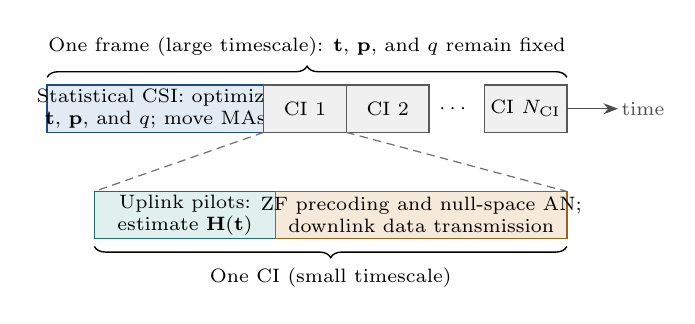
\begin{tikzpicture}[font=\scriptsize, >=Stealth, x=1cm, y=1cm]
  % one frame (large timescale)
  \draw[fill=fblue!14, draw=fblue!70!black, line width=0.5pt] (0,1.35) rectangle (2.75,1.95);
  \node[align=center] at (1.375,1.65) {Statistical CSI: optimize\\$\mathbf t$, $\mathbf p$, and $q$; move MAs};
  \foreach \a/\t in {2.75/CI $1$, 3.8/CI $2$, 5.55/CI $N_{\mathrm{CI}}$}{
    \draw[fill=black!6, draw=black!65, line width=0.5pt] (\a,1.35) rectangle (\a+1.05,1.95);
    \node at (\a+0.525,1.65) {\t};}
  \node at (5.175,1.65) {$\cdots$};
  \draw[->, black!70, line width=0.5pt] (6.6,1.65) -- (7.25,1.65) node[right, inner sep=1pt] {time};
  \draw[decorate, decoration={brace, amplitude=4pt}, line width=0.5pt] (0,2.05) -- (6.6,2.05)
     node[midway, above=4pt] {One frame (large timescale): $\mathbf t$, $\mathbf p$, and $q$ remain fixed};
  % one CI (small timescale)
  \draw[black!55, densely dashed, line width=0.45pt] (2.75,1.35) -- (0.6,0.6);
  \draw[black!55, densely dashed, line width=0.45pt] (3.8,1.35) -- (6.6,0.6);
  \draw[fill=fteal!15, draw=fteal!70!black, line width=0.5pt] (0.6,0) rectangle (2.9,0.6);
  \node[align=center] at (1.75,0.3) {Uplink pilots:\\estimate $\mathbf H(\mathbf t)$};
  \draw[fill=fochre!18, draw=fochre!75!black, line width=0.5pt] (2.9,0) rectangle (6.6,0.6);
  \node[align=center] at (4.75,0.3) {ZF precoding and null-space AN;\\downlink data transmission};
  \draw[decorate, decoration={brace, mirror, amplitude=4pt}, line width=0.5pt] (0.6,-0.1) -- (6.6,-0.1)
     node[midway, below=4pt] {One CI (small timescale)};
\end{tikzpicture}
\caption{Two-timescale transmission protocol.}
\label{fig:protocol}
\end{figure}

Unlike the instantaneous CSI over the entire region $\mathcal C$, the statistical CSI, i.e., $\{\beta_m,\kappa_m,\theta_m,\phi_m\}_{m\in\mathcal M}$ of the LUs and $\{\beta_{\mathrm{e}},\kappa_{\mathrm{e}},\theta_{\mathrm{e}},\phi_{\mathrm{e}}\}$ of Eve, is determined by the large-scale fading and the LoS geometry, which vary much more slowly than the small-scale fading. Following~\cite{HuTMC2024,ChenArxiv2026}, we assume that the statistical CSI of Eve is known at the BS.\footnote{The statistical CSI of Eve can be obtained, e.g., from the prior knowledge of the location of Eve, by sensing its direction~\cite{ChenArxiv2026}, or from its historical signals if it is an untrusted node.}

Accordingly, we adopt the two-timescale protocol in Fig.~\ref{fig:protocol}. Each frame contains $N_{\mathrm{CI}}\gg1$ CIs with fixed statistical CSI. At the beginning of the frame, the BS optimizes the antenna positions $\bt$ and the long-term power allocation $(\bp,q)$ (see Section~\ref{sec:zfan}) and moves the MAs to the selected positions. In each CI, uplink pilots and time-division-duplex channel reciprocity provide $\bH(\bt)$ at the selected positions, from which the BS constructs the precoders and AN covariance. The LU CSI is assumed perfect, whereas $\gtl$ is unavailable at the BS. The rate objective measures spectral efficiency during data transmission and excludes the movement delay, movement energy, and pilot overhead. The position constraints describe feasible stationary configurations; antenna trajectories and collision avoidance during repositioning are outside the model. The MAs are repositioned once per frame, and instantaneous LU CSI is required only at the selected configuration.

\subsection{Signal Model and Ergodic Secrecy Rate}

In each CI, the BS transmits the confidential symbols $s_m\sim\CN(0,1)$, $m\in\mathcal M$, together with AN, and the transmit signal is given by
\begin{equation}\label{eq:x}
\bx=\sum_{m=1}^{M}\bw_m s_m+\bz,
\end{equation}
where $\bw_m\in\mathbb C^{N\times1}$ is the precoding vector for the $m$-th LU, and $\bz\sim\CN(\mathbf 0,\bSig)$ is the AN with covariance matrix $\bSig\succeq\mathbf 0$. The symbols $s_1,\ldots,s_M$ and the AN $\bz$ are mutually independent. The transmit power satisfies $\sum_{m=1}^M\|\bw_m\|^2+\tr(\bSig)\le\Ptot$, where $\Ptot$ is the maximum transmit power of the BS. Under the two-timescale protocol, $\bw_m$ and $\bSig$ depend on the instantaneous CSI of the LUs and are thus denoted by $\bw_m(\bH(\bt))$ and $\bSig(\bH(\bt))$.

The signal received at the $m$-th LU is $y_m=\bh_m^{\mathrm{H}}(\bt)\bx+n_m$, where $n_m\sim\CN(0,\sigma_m^2)$ is the additive white Gaussian noise. The resulting SINR of the $m$-th LU is
\begin{align}
I_m&\triangleq\sum_{\substack{i=1\\ i\neq m}}^{M}
 |\bh_m^{\mathrm{H}}(\bt)\bw_i|^2
 +\bh_m^{\mathrm{H}}(\bt)\bSig\bh_m(\bt),\nonumber\\
\gamma_m&=\frac{|\bh_m^{\mathrm{H}}(\bt)\bw_m|^2}{I_m+\sigma_m^2}.
\label{eq:sinr_gen}
\end{align}
The signal received at Eve is $y_{\mathrm{e}}=\bg^{\mathrm{H}}(\bt)\bx+n_{\mathrm{e}}$ with $n_{\mathrm{e}}\sim\CN(0,\sigma_{\mathrm{e}}^2)$. Since the receiver of a passive Eve is unknown to the BS, we consider the worst case where Eve can cancel the signals of the other LUs when intercepting $s_m$, e.g., via multiuser detection~\cite{ZhuTWC2014}. This worst-case model yields a secrecy guarantee regardless of the decoding capability of Eve. The SINR of Eve for $s_m$ is then
\begin{equation}\label{eq:sinre_gen}
\gamma_{\mathrm{e},m}=\frac{|\bg^{\mathrm{H}}(\bt)\bw_m|^2}{\bg^{\mathrm{H}}(\bt)\bSig\bg(\bt)+\sigma_{\mathrm{e}}^2},
\end{equation}
which upper-bounds that of an Eve treating the signals of the other LUs as interference.

Since the instantaneous CSI of Eve is unknown, the confidential message of each LU is encoded across independently faded CIs with fixed statistical CSI and fixed long-term variables. We use the asymptotic stationary-ergodic coding model in~\cite{Gopala2008,ZhuTWC2014}, under which the following ergodic secrecy rate is achievable for the $m$-th LU:
\begin{equation}\label{eq:esr}
R_m^{\mathrm{sec}}\triangleq\big[\bar R_m-\bar R_{\mathrm{e},m}\big]^+,
\end{equation}
where $\bar R_m$ is the ergodic rate of LU $m$ and $\bar R_{\mathrm{e},m}$ is the ergodic wiretap rate for $s_m$, defined as
\begin{equation}\label{eq:ergodic}
\begin{aligned}
\bar R_m&\triangleq\E\{\log_2(1+\gamma_m)\},\\
\bar R_{\mathrm{e},m}&\triangleq\E\{\log_2(1+\gamma_{\mathrm{e},m})\}.
\end{aligned}
\end{equation}
Both expectations are taken over $\Htl$ and $\gtl$ for fixed $\bt$. The ESSR is $\sum_{m=1}^{M}R_m^{\mathrm{sec}}$.

\subsection{Problem Formulation}

We aim to maximize the ESSR by jointly optimizing the antenna positions and the short-timescale policy $\mathcal W\triangleq\{\bw_1(\bH(\bt)),\ldots,\bw_M(\bH(\bt)),\bSig(\bH(\bt))\}$, i.e., the mapping from the instantaneous CSI of the LUs to the precoders and the AN covariance matrix. The corresponding problem is formulated as
\begin{subequations}\label{eq:P1}
\begin{align}
(\mathrm{P1}):\ \max_{\bt,\,\mathcal W}\ \ & \sum_{m=1}^{M}R_m^{\mathrm{sec}}\label{eq:P1obj}\\
\mathrm{s.t.}\ \ & \sum_{m=1}^M\big\|\bw_m(\bH(\bt))\big\|^2+\tr\big(\bSig(\bH(\bt))\big)\le\Ptot,\nonumber\\
& \bSig(\bH(\bt))\succeq\mathbf 0,\ \forall\bH(\bt),\label{eq:P1pow}\\
& \bt_n\in\mathcal C,\ \forall n\in\mathcal N,\label{eq:P1region}\\
& \|\bt_n-\bt_i\|\ge\Dmin,\ \forall n,i\in\mathcal N,\ n\neq i.\label{eq:P1dist}
\end{align}
\end{subequations}
Here, \eqref{eq:P1pow} must hold for every realization of $\bH(\bt)$.

Problem (P1) is difficult to solve for two reasons. First, the ergodic rates in~\eqref{eq:ergodic} have no closed-form expressions, and the policy $\mathcal W$ has to be designed for every realization of $\bH(\bt)$. Second, since the phases of the LoS components in~\eqref{eq:hbar} vary with $\bt$, the objective function is nonconcave in $\bt$, and the minimum-distance constraints in~\eqref{eq:P1dist} are nonconvex. To address the first difficulty, Section~\ref{sec:analysis} restricts $\mathcal W$ to ZF precoding and null-space AN with a long-term power allocation and approximates the ergodic rates in closed form, thereby yielding a deterministic problem w.r.t.\ the long-term variables only. To address the second difficulty, Section~\ref{sec:opt} develops an AO algorithm for this problem.

% =============================================================================
\section{Two-Timescale ZF-AN Design and Ergodic Secrecy Rate Analysis}\label{sec:analysis}
% =============================================================================

\subsection{Short-Timescale ZF Precoding and Null-Space AN}\label{sec:zfan}

We restrict the short-timescale policy to ZF precoding and null-space AN with a long-term power allocation. In each CI, the precoder for LU $m$ is $\bw_m(\bH(\bt))=\sqrt{p_m}\,\wb_m$, where $p_m\ge0$ is its allocated power. Define the unnormalized and unit-norm ZF directions as
\begin{equation}\label{eq:zf}
\begin{aligned}
\bw_m^\circ&\triangleq\bH(\bt)
 \big(\bH^{\mathrm{H}}(\bt)\bH(\bt)\big)^{-1}\be_m,\\
\wb_m&\triangleq\frac{\bw_m^\circ}{\|\bw_m^\circ\|}.
\end{aligned}
\end{equation}
The direction satisfies $\bh_i^{\mathrm{H}}(\bt)\wb_m=0$ for $i\neq m$. The AN covariance is $\bSig(\bH(\bt))=q\,\PHp$, with $q\ge0$ denoting the AN power per null-space dimension~\cite{Zhou2010,ZhuTWC2014}. The projector onto the null space of $\bH^{\mathrm{H}}(\bt)$ is
\begin{equation}\label{eq:an}
\PHp=\bI_N-\bH(\bt)
 \big(\bH^{\mathrm{H}}(\bt)\bH(\bt)\big)^{-1}\bH^{\mathrm{H}}(\bt).
\end{equation}
For finite Rician factors, positive large-scale gains, and $N>M$, the independent Gaussian NLoS components imply that $\bH(\bt)$ has full column rank almost surely. Therefore, $\bH^{\mathrm{H}}(\bt)\PHp=\mathbf 0$ and $\tr(\PHp)=N-M$ almost surely. The AN causes no interference to the LUs, and the transmit power in each CI is $\sum_{m=1}^M p_m+(N-M)q$. On a rank-deficient channel realization, which has probability zero under this model, define the policy by $\bw_m=\mathbf 0$ for all $m$ and $\bSig=\mathbf 0$. This extension satisfies the every-realization power constraint in (P1) and does not change any ergodic rate. We assume $\beta_{\mathrm{e}}>0$, $0\le\kappa_{\mathrm{e}}<\infty$, $\sigma_m^2>0$, and $\sigma_{\mathrm{e}}^2>0$ throughout the finite-parameter analysis; infinite Rician factors are considered only as limits.

In numerical evaluation, a nonfinite or unsafe Gram-matrix pivot, or an estimated reciprocal infinity-norm condition number no larger than $10^{-12}$, triggers an explicit experiment failure. No channel realization is discarded or redrawn; this numerical threshold is distinct from the probability-zero rank-deficient set.

We refer to $\bp\triangleq[p_1,\ldots,p_M]^{\mathrm{T}}$ and $q$ as the long-term power allocation, which is optimized based on the statistical CSI and remains fixed within a frame. In contrast, $\wb_m$ and $\PHp$ are updated in each CI according to $\bH(\bt)$. With this design, the SINRs in~\eqref{eq:sinr_gen} and~\eqref{eq:sinre_gen} reduce to
\begin{align}
\gamma_m&=\frac{p_m|\bh_m^{\mathrm{H}}(\bt)\wb_m|^2}{\sigma_m^2}
\nonumber\\
&=\frac{p_m}{\sigma_m^2
 \big[(\bH^{\mathrm{H}}(\bt)\bH(\bt))^{-1}\big]_{m,m}},
\label{eq:snr}\\
\gamma_{\mathrm{e},m}&=\frac{p_m|\bg^{\mathrm{H}}(\bt)\wb_m|^2}
 {q\,\bg^{\mathrm{H}}(\bt)\PHp\bg(\bt)+\sigma_{\mathrm{e}}^2},
\label{eq:sinre}
\end{align}
where the second equality in~\eqref{eq:snr} follows from $|\bh_m^{\mathrm{H}}(\bt)\wb_m|^2=1/[(\bH^{\mathrm{H}}(\bt)\bH(\bt))^{-1}]_{m,m}$ by~\eqref{eq:zf}.

The adopted ZF-AN design requires only the instantaneous CSI of the LUs, and no optimization problem needs to be solved in each CI, since $\bp$ and $q$ depend only on the statistical CSI. Moreover, the equal power allocation in~\cite{ZhengTCOM2025} and the information--AN power splitting with equal power per LU are special cases of $(\bp,q)$. With the ZF-AN design, (P1) is restricted to
\begin{subequations}\label{eq:P2}
\begin{align}
(\mathrm{P2}):\ \max_{\bt,\bp,q}\ \ & \sum_{m=1}^{M}R_m^{\mathrm{sec}}(\bt,p_m,q)\label{eq:P2obj}\\
\mathrm{s.t.}\ \ & \sum_{m=1}^{M}p_m+(N-M)q\le\Ptot,\label{eq:P2pow}\\
& p_m\ge0,\ \forall m\in\mathcal M,\quad q\ge0,\label{eq:P2pos}\\
& \bt_n\in\mathcal C,\ \forall n\in\mathcal N,\label{eq:P2region}\\
& \|\bt_n-\bt_i\|\ge\Dmin,\ \forall n,i\in\mathcal N,\ n\neq i,\label{eq:P2dist}
\end{align}
\end{subequations}
where $R_m^{\mathrm{sec}}(\bt,p_m,q)$ denotes~\eqref{eq:esr} with the SINRs in~\eqref{eq:snr} and~\eqref{eq:sinre}, and~\eqref{eq:P2pow} and~\eqref{eq:P2pos} guarantee~\eqref{eq:P1pow} in every CI. Since the ZF-AN design is a particular policy $\mathcal W$, every feasible solution of (P2) is feasible for (P1), i.e., (P2) is a restriction of (P1). However, (P2) is still intractable, since the ergodic rates in~\eqref{eq:P2obj} have no closed-form expressions. Next, we approximate the ergodic rates of the LUs and Eve in Sections~\ref{sec:lu} and~\ref{sec:eve}, respectively.

\subsection{Ergodic Rate of the LUs}\label{sec:lu}

Define $\bB\triangleq\diag\big(\frac{\beta_1}{\kappa_1+1},\ldots,\frac{\beta_M}{\kappa_M+1}\big)$ and $\bL(\bt)\triangleq\Hb(\bt)\bK^{1/2}$. From~\eqref{eq:hm}, the channel matrix of the LUs can be written as
\begin{equation}\label{eq:Hdecomp}
\bH(\bt)=\big(\bL(\bt)+\Htl\big)\bB^{1/2},
\end{equation}
where $\bL(\bt)+\Htl$ is the normalized channel matrix, whose LoS component is weighted by the square roots of the Rician factors. Accordingly, we define
\begin{equation}\label{eq:Phi}
\begin{aligned}
\bPhi(\bt)&\triangleq\bL^{\mathrm{H}}(\bt)\bL(\bt)+N\bI_M,\\
\bOm(\bt)&\triangleq\bPhi^{-1}(\bt),
\end{aligned}
\end{equation}
where $\bPhi(\bt)=\E\{(\bL(\bt)+\Htl)^{\mathrm{H}}(\bL(\bt)+\Htl)\}$ is the correlation matrix of the normalized channels of the LUs. The ergodic rate of the LUs under ZF precoding has been characterized in~\cite{ZhangJSTSP2014,ZhengTCOM2025}, and the result is restated below for completeness.

\begin{lemma}[{\cite{ZhangJSTSP2014,ZhengTCOM2025}}]\label{lem:lu}
For given $\bt$ and $p_m$, the ergodic rate of the $m$-th LU is approximated by
\begin{equation}\label{eq:Rm}
\bar R_m\approx\tilde R_m(\bt,p_m)\triangleq\log_2\big(1+\eta_m(\bt)\,p_m\big),
\end{equation}
where $\eta_m(\bt)\triangleq\zeta_m(N-M)/(N\omega_m(\bt))$ is the effective channel gain of the $m$-th LU, $\zeta_m\triangleq\beta_m/((\kappa_m+1)\sigma_m^2)$, and $\omega_m(\bt)\triangleq[\bOm(\bt)]_{m,m}$.
\end{lemma}

To distinguish the exact inequality from the subsequent moment approximation, let $Z_m\triangleq[(\bH^{\mathrm{H}}(\bt)\bH(\bt))^{-1}]_{m,m}$. Since $\log_2(1+p_m/(\sigma_m^2 z))$ is convex for $z>0$, Jensen's inequality gives
\begin{equation}\label{eq:lu_jensen_exact}
\bar R_m\ge
\log_2\!\left(1+\frac{p_m}{\sigma_m^2\E\{Z_m\}}\right).
\end{equation}
The central Wishart approximation in~\cite{ZhangJSTSP2014} replaces the noncentral Gram matrix of $\bL(\bt)+\Htl$ by a central Wishart matrix with $N$ degrees of freedom and covariance $\bPhi(\bt)/N$. Its inverse moment gives $\E\{Z_m\}\approx N\omega_m(\bt)/((N-M)[\bB]_{m,m})$, which yields~\eqref{eq:Rm} and is equivalent to~\cite[Sec.~IV-A]{ZhengTCOM2025}. The inverse-moment substitution is an approximation, so~\eqref{eq:Rm} is not asserted to be a lower bound for an arbitrary noncentral channel. For Rayleigh fading, the inverse moment is exact and~\eqref{eq:Rm} reduces to the lower bound $\log_2(1+\zeta_mp_m(N-M))$~\cite{Ngo2013}. Its behavior in the LoS-dominant regime is evaluated in Section~\ref{sec:sim_acc}. The antenna positions affect $\tilde R_m(\bt,p_m)$ only through $\omega_m(\bt)$. Since $\bPhi(\bt)\succeq N\bI_M$ and $[\bOm(\bt)]_{m,m}\ge1/[\bPhi(\bt)]_{m,m}=1/(N(\kappa_m+1))$~\cite{Horn2013}, we have
\begin{equation}\label{eq:etabound}
\zeta_m(N-M)\le\eta_m(\bt)\le\zeta_m(N-M)(\kappa_m+1),
\end{equation}
where the upper bound is achieved if $\hb_m^{\mathrm{H}}(\bt)\hb_i(\bt)=0$ for all $i\neq m$ with $\kappa_i>0$. Hence, $1/(N\omega_m(\bt))\in[1,\kappa_m+1]$ is the LoS gain of the $m$-th LU that survives the ZF precoding. The antenna positions can improve this gain by decorrelating the LoS components of the LUs.

\subsection{Ergodic Wiretap Rate of Eve}\label{sec:eve}

Unlike $\gamma_m$ in~\eqref{eq:snr}, which depends on $\bH(\bt)$ only through $[(\bH^{\mathrm{H}}(\bt)\bH(\bt))^{-1}]_{m,m}$, the SINR of Eve in~\eqref{eq:sinre} depends on the random ZF direction $\wb_m$ and AN subspace, both determined by $\bH(\bt)$. This dependence is the main difficulty in deriving $\bar R_{\mathrm{e},m}$. To address this issue, we first characterize the information leakage and the AN received by Eve given $\bH(\bt)$.

\begin{lemma}\label{lem:indep}
Conditioned on $\bH(\bt)$, the information leakage $X_m\triangleq|\bg^{\mathrm{H}}(\bt)\wb_m|^2$ and the AN power $Y\triangleq\bg^{\mathrm{H}}(\bt)\PHp\bg(\bt)$ received by Eve are independent, and their conditional means and variances are given by
\begin{align}
\E\{X_m|\bH(\bt)\}&=\tilde\beta_{\mathrm{e}}\big(\kappa_{\mathrm{e}}\bar X_m+1\big),\nonumber\\
\mathrm{Var}\{X_m|\bH(\bt)\}&=\tilde\beta_{\mathrm{e}}^2\big(2\kappa_{\mathrm{e}}\bar X_m+1\big),\label{eq:EX}\\
\E\{Y|\bH(\bt)\}&=\tilde\beta_{\mathrm{e}}\big(\kappa_{\mathrm{e}}\bar Y+N-M\big),\nonumber\\
\mathrm{Var}\{Y|\bH(\bt)\}&=\tilde\beta_{\mathrm{e}}^2\big(2\kappa_{\mathrm{e}}\bar Y+N-M\big),\label{eq:EY}
\end{align}
where $\tilde\beta_{\mathrm{e}}\triangleq\beta_{\mathrm{e}}/(\kappa_{\mathrm{e}}+1)$, and $\bar X_m\triangleq|\gb^{\mathrm{H}}(\bt)\wb_m|^2$ and $\bar Y\triangleq\gb^{\mathrm{H}}(\bt)\PHp\gb(\bt)$ are the LoS counterparts of $X_m$ and $Y$.
\end{lemma}
\begin{IEEEproof}
See Appendix~\ref{app:indep}.
\end{IEEEproof}

Lemma~\ref{lem:indep} follows from the isotropic Gaussian covariance of Eve's NLoS component and the orthogonality between the ZF direction and the AN subspace. It does not imply unconditional independence after averaging over $\Htl$. Indeed, the laws of total variance and total covariance give
\begin{align}
\frac{\mathrm{Var}\{X_m\}}{\tilde\beta_{\mathrm{e}}^2}
&=1+2\kappa_{\mathrm{e}}\E\{\bar X_m\}
  +\kappa_{\mathrm{e}}^2\mathrm{Var}\{\bar X_m\},\nonumber\\
\frac{\mathrm{Var}\{Y\}}{\tilde\beta_{\mathrm{e}}^2}
&=N-M+2\kappa_{\mathrm{e}}\E\{\bar Y\}
  +\kappa_{\mathrm{e}}^2\mathrm{Var}\{\bar Y\},\nonumber\\
\frac{\mathrm{Cov}\{X_m,Y\}}{\tilde\beta_{\mathrm{e}}^2}
&=\kappa_{\mathrm{e}}^2\mathrm{Cov}\{\bar X_m,\bar Y\}.
\label{eq:unconditional_moments}
\end{align}
Thus, small conditional relative variances alone do not establish concentration of the unconditional received powers: their conditional means also vary with the LU channel. To obtain a deterministic design objective, we apply a first-order moment approximation to $\log_2(1+p_mX_m/(qY+\sigma_{\mathrm{e}}^2))$, replacing the received powers by their unconditional means, as motivated by~\cite[Lemma~1]{ZhangJSTSP2014}. This replacement is neither an equality nor a general upper or lower bound, because the logarithmic rate is concave in $X_m$ and convex in $Y$ for $p_m,q>0$. Its accuracy must therefore be checked against the exact SINR, including weak-LoS and small-null-space cases. Substitution of the exact conditional means in Lemma~\ref{lem:indep} yields
\begin{equation}\label{eq:Re0}
\bar R_{\mathrm{e},m}\approx\log_2\bigg(1+\frac{p_m\big(\kappa_{\mathrm{e}}\E\{\bar X_m\}+1\big)}{q\big(\kappa_{\mathrm{e}}\E\{\bar Y\}+N-M\big)+\sbe}\bigg),
\end{equation}
where $\sbe\triangleq\sigma_{\mathrm{e}}^2/\tilde\beta_{\mathrm{e}}$ is the normalized noise power of Eve.

However, $\E\{\bar X_m\}$ and $\E\{\bar Y\}$ in~\eqref{eq:Re0}, i.e., the average LoS energies of Eve along the ZF direction of the $m$-th LU and in the AN subspace, respectively, still have no closed-form expressions. Since $\wb_m$ and $\PHp$ are invariant to the scaling of the columns of $\bH(\bt)$, they depend on $\bH(\bt)$ only through the normalized channel matrix $\bL(\bt)+\Htl$ in~\eqref{eq:Hdecomp}. We approximate $\E\{\bar X_m\}$ and $\E\{\bar Y\}$ by replacing the inverse of the random Gram matrix of $\bL(\bt)+\Htl$ with the inverse of its mean $\bPhi(\bt)$, where the NLoS contribution to the AN subspace is calibrated by the identity $\tr(\PHp)=N-M$. These approximations lead to the following result.

\begin{proposition}\label{prop:eve}
The average LoS energies in~\eqref{eq:Re0} are approximated by $\E\{\bar X_m\}\approx c_m(\bt)$ and $\E\{\bar Y\}\approx d(\bt)$, where
\begin{align}
c_m(\bt)&\triangleq
 \frac{\big|[\bOm(\bt)\bv(\bt)]_m\big|^2}
 {\omega_m(\bt)}\nonumber\\
&\quad+\frac{N[\bOm^2(\bt)]_{m,m}}{\omega_m(\bt)},
\label{eq:cm}\\
d(\bt)&\triangleq\frac{N-M}
 {N-M+N\tr(\bOm(\bt))}\nonumber\\
&\quad\times\big(N-\bv^{\mathrm{H}}(\bt)\bOm(\bt)\bv(\bt)\big),
\label{eq:d}
\end{align}
and $\bv(\bt)\triangleq\bL^{\mathrm{H}}(\bt)\gb(\bt)=\bK^{1/2}\Hb^{\mathrm{H}}(\bt)\gb(\bt)$. Accordingly, the ergodic wiretap rate of Eve for $s_m$ is approximated by
\begin{equation}\label{eq:Re}
\bar R_{\mathrm{e},m}\approx\tilde R_{\mathrm{e},m}(\bt,p_m,q)\triangleq\log_2\bigg(1+\frac{\xi_m(\bt)\,p_m}{q\,\psi(\bt)+\sbe}\bigg),
\end{equation}
where $\xi_m(\bt)\triangleq\kappa_{\mathrm{e}}c_m(\bt)+1$ and $\psi(\bt)\triangleq\kappa_{\mathrm{e}}d(\bt)+N-M$.
\end{proposition}
\begin{IEEEproof}
See Appendix~\ref{app:det}.
\end{IEEEproof}

The approximations of $\E\{\bar X_m\}$ and $\E\{\bar Y\}$ in Proposition~\ref{prop:eve} are exact when all LU LoS components vanish, and their values lie in $[0,N]$ (see Appendix~\ref{app:det}). Their large-LoS exactness requires a fixed, full-column-rank limiting LU LoS matrix, as specified in Lemma~\ref{lem:det}; it does not cover coincident or linearly dependent limiting LU steering vectors. The corresponding rate approximation in~\eqref{eq:Re} has an additional moment-replacement error and is not exact merely because the LU channels are Rayleigh. If all LU channels and Eve's channel approach deterministic LoS channels with a full-column-rank limiting LU matrix and positive noise powers, the random ZF directions and the AN subspace converge to their deterministic counterparts, and the wiretap-rate approximation also becomes exact. No uniform accuracy statement is made near a rank-deficient limiting LU geometry. The coefficients $\xi_m(\bt)$ and $\psi(\bt)$ describe normalized leakage and normalized AN reception in the adopted approximation. The vector $\bv(\bt)$ retains the LoS correlation between Eve and the LUs, which is absent from an approximation based only on the diagonal of $\bOm(\bt)$.

\subsection{Approximate ESSR Maximization Problem}\label{sec:discussion}

Based on Lemma~\ref{lem:lu} and Proposition~\ref{prop:eve}, the ergodic secrecy rate of the $m$-th LU is approximated by
\begin{equation}\label{eq:esrapprox}
\begin{aligned}
R_m^{\mathrm{sec}}&\approx\tilde R_m^{\mathrm{sec}}(\bt,p_m,q)\\
&\triangleq\big[\tilde R_m(\bt,p_m)
 -\tilde R_{\mathrm{e},m}(\bt,p_m,q)\big]^+,
\end{aligned}
\end{equation}
which depends only on the statistical CSI and is thus suitable for the large-timescale design. The following remarks reveal how the antenna positions affect the approximate ESSR.

\begin{remark}[Secrecy Mechanisms of the MAs]\label{rem:mech}
From~\eqref{eq:Rm}, \eqref{eq:cm}, and~\eqref{eq:d}, the antenna positions affect the approximate ESSR via $\omega_m(\bt)$, $c_m(\bt)$, and $d(\bt)$, i.e., via the LoS array correlations $[\Hb^{\mathrm{H}}(\bt)\Hb(\bt)]_{i,j}=\sum_{n=1}^{N}e^{j\frac{2\pi}{\lambda}\bt_n^{\mathrm{T}}(\ba_j-\ba_i)}$ among the LUs and $[\Hb^{\mathrm{H}}(\bt)\gb(\bt)]_{i}=\sum_{n=1}^{N}e^{j\frac{2\pi}{\lambda}\bt_n^{\mathrm{T}}(\ba_{\mathrm{e}}-\ba_i)}$ between Eve and the LUs. A smaller $\omega_m(\bt)$, i.e., a weaker LoS correlation between the $m$-th LU and the other LUs, yields a larger ZF gain in~\eqref{eq:etabound}. This decorrelation among the LUs is the only mechanism exploited by the rate-oriented design~\cite{ZhengTCOM2025}. In secure transmission, a smaller $c_m(\bt)$ and a larger $d(\bt)$ provide two additional mechanisms, i.e., less information leakage and more AN received by Eve. In particular, if $\bv(\bt)=\mathbf 0$, i.e., the LoS component of Eve is orthogonal to those of all the LUs, then $c_m(\bt)$ reduces to its minimum $N[\bOm^2(\bt)]_{m,m}/\omega_m(\bt)$ caused by the NLoS components, and $d(\bt)$ achieves its maximum $N(N-M)/(N-M+N\tr(\bOm(\bt)))$ for a given $\bPhi(\bt)$. Hence, by decorrelating the LoS component of Eve from those of the LUs, the MAs simultaneously reduce the information leakage and increase the AN received by Eve, whereas an FPA array can hardly achieve this decorrelation when Eve is located in a direction close to that of an LU. Note that if $\kappa_{\mathrm{e}}=0$, then $\tilde R_{\mathrm{e},m}=\log_2(1+p_m/(q(N-M)+\sbe))$ does not depend on $\bt$, i.e., the statistical CSI of Eve carries no spatial information, and only the first mechanism remains.
\end{remark}

\begin{remark}[Single LU]\label{rem:single}
For $M=1$, the sole entry of $\bPhi(\bt)$ is $[\bPhi(\bt)]_{1,1}=N(\kappa_1+1)$, so $\eta_1=\zeta_1(N-1)(\kappa_1+1)$ is independent of $\bt$.\footnote{For $M=1$, the exact ergodic rate $\E\{\log_2(1+p_1\|\bh_1(\bt)\|^2/\sigma_1^2)\}$ is also independent of $\bt$, because the distribution of $\|\bh_1(\bt)\|^2$ depends on $\hb_1(\bt)$ only through $\|\hb_1(\bt)\|^2=N$.} In contrast,
\begin{align}
c_1(\bt)&=\frac{\kappa_1|\hb_1^{\mathrm{H}}(\bt)\gb(\bt)|^2/N+1}
 {\kappa_1+1},\label{eq:c1}\\
d(\bt)&=\frac{(N-1)(\kappa_1+1)}
 {(N-1)(\kappa_1+1)+1}\nonumber\\
&\quad\times\bigg(N-
 \frac{\kappa_1|\hb_1^{\mathrm{H}}(\bt)\gb(\bt)|^2}
 {N(\kappa_1+1)}\bigg).\label{eq:d1}
\end{align}
Both quantities depend on $\bt$ through the LoS correlation $|\hb_1^{\mathrm{H}}(\bt)\gb(\bt)|^2$ between the LU and Eve. Reducing this correlation decreases $c_1(\bt)$ and increases $d(\bt)$ in the adopted approximation, whereas the LU rate is position-independent~\cite[Remark~2]{ZhengTCOM2025}. For a single LU, however, the exact projectors satisfy $\wb_1\wb_1^{\mathrm{H}}+\PHp=\bI_N$ and hence $\bar X_1+\bar Y=N$ for every channel realization. The separately constructed approximations do not enforce this identity at finite $\kappa_1$: writing $C_1\triangleq|\hb_1^{\mathrm{H}}(\bt)\gb(\bt)|^2$, their residual is
\begin{equation}\label{eq:single_identity_residual}
c_1+d-N=
\frac{\kappa_1(C_1/N-1)}
{(\kappa_1+1)((N-1)(\kappa_1+1)+1)}.
\end{equation}
Thus, the single-user secrecy trend is a prediction of the approximation that requires verification using the exact SINRs. The residual vanishes in the Rayleigh and deterministic-LoS limits but is generally nonzero between these limits.
\end{remark}

\begin{remark}[High-SNR Behavior and AN Saving]\label{rem:highsnr}
Consider the information--AN power splitting with equal power among the LUs, i.e., $p_m=\alpha\Ptot/M$ and $q=(1-\alpha)\Ptot/(N-M)$, where $\alpha\in(0,1)$ is the power-splitting factor. In the high SNR regime, i.e., as $\Ptot\to\infty$, we have
\begin{equation}\label{eq:highsnr}
\begin{aligned}
\tilde R_m-\tilde R_{\mathrm{e},m}
={}&\log_2\frac{\alpha\Ptot\eta_m(\bt)}{M}\\
&-\log_2\Big(1+\frac{\alpha\Theta_m(\bt)}
 {1-\alpha}\Big)+o(1),
\end{aligned}
\end{equation}
where $o(1)$ vanishes as $\Ptot\to\infty$, and $\Theta_m(\bt)\triangleq\frac{(N-M)\xi_m(\bt)}{M\psi(\bt)}$ is the ratio of the normalized information leakage to the normalized AN power received by Eve. Hence, the high-SNR slope of the approximate ESSR equals $M$ regardless of $\bt$, and the antenna positions affect the approximate ESSR only through the constant term. Moreover, the value of $\alpha$ that maximizes the sum of the constant terms in~\eqref{eq:highsnr} satisfies $\sum_{m=1}^M\big[\frac1\alpha-\frac1{1-\alpha}-\frac{\Theta_m-1}{1+\alpha(\Theta_m-1)}\big]=0$, whose solution for $\Theta_m=\Theta$, $\forall m\in\mathcal M$, is given by
\begin{equation}\label{eq:alphastar}
\alpha^\star=\frac{1}{1+\sqrt{\Theta}}.
\end{equation}
Since the MAs can decrease $c_m(\bt)$ and increase $d(\bt)$, they can decrease $\Theta$ and thus increase $\alpha^\star$, i.e., they reduce the AN power required for secure transmission. We refer to this effect as the AN-saving effect.
\end{remark}

Replacing the ergodic secrecy rates in (P2) with~\eqref{eq:esrapprox} yields the following deterministic approximate problem:
\begin{subequations}\label{eq:P3}
\begin{align}
(\mathrm{P3}):\ \max_{\bt,\bp,q}\ \ & F(\bt,\bp,q)\triangleq\sum_{m=1}^{M}\bigg[\log_2\big(1+\eta_m(\bt)p_m\big)\nonumber\\
&\qquad\qquad-\log_2\bigg(1+\frac{\xi_m(\bt)p_m}{q\psi(\bt)+\sbe}\bigg)\bigg]\label{eq:P3obj}\\
\mathrm{s.t.}\ \ & \eqref{eq:P2pow}\text{--}\eqref{eq:P2dist},\nonumber
\end{align}
\end{subequations}
where removing $[\cdot]^+$ preserves the global optimum under freely adjustable nonnegative user powers. For fixed $\bt$ and $q$, each summand depends only on its own $p_m$. Setting $p_m=0$ for every negative summand preserves feasibility, makes those summands zero, and leaves the other summands unchanged. Therefore, (P3) and its positive-part counterpart have the same global optimum. This argument does not identify $F$ with the approximate ESSR at an arbitrary intermediate position iterate: a position update with fixed powers can make an individual summand negative. Accordingly, Algorithm~\ref{alg:ao} monitors the smooth objective $F$; Monte Carlo evaluation retains $[\cdot]^+$ as in~\eqref{eq:esr}. For a final report of the approximate ESSR, evaluate~\eqref{eq:esrapprox} directly. Under equal user powers, turning off a single user is inadmissible, so the positive-part operator must also be retained during benchmark optimization.

% =============================================================================
\section{Proposed Two-Timescale Optimization Algorithm}\label{sec:opt}
% =============================================================================
Problem (P3) is still nonconvex, since $F$ is nonconcave w.r.t.\ $\bt$ and the minimum-distance constraints in~\eqref{eq:P2dist} are nonconvex. Moreover, $\bt$, $\bp$, and $q$ are coupled in the objective function, and $\bp$ and $q$ are further coupled by the power constraint~\eqref{eq:P2pow}. Nevertheless, (P3) has two useful structures. First, for given $\bt$, the coefficients $\eta_m$, $\xi_m$, and $\psi$ in~\eqref{eq:P3obj} are constants, and the optimal power allocation among the LUs for a given $q$ can be derived in semi-closed form. Second, for given $\bp$ and $q$, each antenna position affects $F$ only through a rank-one update of $\bPhi(\bt)$ and $\bv(\bt)$, which renders a global search for each position affordable. Based on these structures, we alternately optimize the power allocation and the antenna positions in Sections~\ref{sec:power} and~\ref{sec:position}, respectively.

\subsection{Power Allocation Optimization for Given $\bt$}\label{sec:power}

For given $\bt$, (P3) reduces to
\begin{subequations}\label{eq:P31}
\begin{align}
(\mathrm{P3.1}):\ \max_{\bp,q}\ \ & \sum_{m=1}^{M}f_m(p_m;q)\\
\mathrm{s.t.}\ \ & \eqref{eq:P2pow},\ \eqref{eq:P2pos},\nonumber
\end{align}
\end{subequations}
where
\begin{equation}\label{eq:fm}
f_m(p;q)\triangleq\log_2(1+\eta_mp)-\log_2\big(1+\eta_{\mathrm{e},m}(q)\,p\big),
\end{equation}
and $\eta_{\mathrm{e},m}(q)\triangleq\xi_m/(q\psi+\sbe)$, which decreases with $q$, is the effective channel gain of Eve for $s_m$. Problem (P3.1) is nonconvex in general, because $f_m$ is not jointly concave in $p_m$ and $q$. Nevertheless, for a given $q$, its optimal $\bp$ can be obtained in semi-closed form, as shown below. The first-order and second-order derivatives of $f_m$ w.r.t.\ $p$ are given by
\begin{align}
\frac{\partial f_m}{\partial p}&=\frac{\eta_m-\eta_{\mathrm{e},m}}{\ln2\,(1+\eta_mp)(1+\eta_{\mathrm{e},m}p)},\label{eq:fm1}\\
\frac{\partial^2 f_m}{\partial p^2}&=\frac{1}{\ln2}\bigg[\frac{\eta_{\mathrm{e},m}^2}{(1+\eta_{\mathrm{e},m}p)^2}-\frac{\eta_m^2}{(1+\eta_mp)^2}\bigg],\label{eq:fm2}
\end{align}
where the argument $q$ of $\eta_{\mathrm{e},m}$ is omitted. If $\eta_m\le\eta_{\mathrm{e},m}$, then $f_m(p;q)\le0$ for all $p\ge0$, and thus $p_m=0$ is optimal. If $\eta_m>\eta_{\mathrm{e},m}$, then $\eta_m(1+\eta_{\mathrm{e},m}p)-\eta_{\mathrm{e},m}(1+\eta_mp)=\eta_m-\eta_{\mathrm{e},m}>0$, i.e., $\frac{\eta_m}{1+\eta_mp}>\frac{\eta_{\mathrm{e},m}}{1+\eta_{\mathrm{e},m}p}$. Hence, by~\eqref{eq:fm1} and~\eqref{eq:fm2}, $f_m$ is strictly increasing and strictly concave in $p\ge0$. Let $\mathcal M_{\mathrm a}(q)\triangleq\{m\in\mathcal M\,|\,\eta_m>\eta_{\mathrm{e},m}(q)\}$ denote the set of LUs that can achieve positive secrecy rates, and $P_{\mathrm I}(q)\triangleq\Ptot-(N-M)q$ the power available for the confidential signals. Then, the optimal $\bp$ for a given $q$ is given as follows.

\begin{proposition}[Secrecy Water-Filling]\label{prop:wf}
For a given $q$ with $P_{\mathrm I}(q)>0$ and $\mathcal M_{\mathrm a}(q)\neq\emptyset$, the optimal power allocation is $p_m^\star=0$ for $m\notin\mathcal M_{\mathrm a}(q)$ and
\begin{equation}\label{eq:wf}
\begin{aligned}
v_m^{\mathrm{wf}}(\nu)
&\triangleq\sqrt{(\eta_m-\eta_{\mathrm{e},m})^2
 +4\eta_m\eta_{\mathrm{e},m}\rho_m(\nu)},\\
p_m^\star(\nu)
&=\left[\frac{2(\rho_m(\nu)-1)}
 {v_m^{\mathrm{wf}}(\nu)+\eta_m+\eta_{\mathrm{e},m}}\right]^+,
\end{aligned}
\end{equation}
for $m\in\mathcal M_{\mathrm a}(q)$, where $\rho_m=\rho_m(\nu)\triangleq(\eta_m-\eta_{\mathrm{e},m})/(\nu\ln2)$, and the water level $\nu>0$ is the unique solution of $\sum_{m\in\mathcal M_{\mathrm a}(q)}p_m^\star(\nu)=P_{\mathrm I}(q)$.
\end{proposition}
\begin{IEEEproof}
Since the objective is strictly concave and increasing in $\{p_m\}_{m\in\mathcal M_{\mathrm a}(q)}$ and Slater's condition holds, the Karush--Kuhn--Tucker (KKT) conditions are necessary and sufficient for optimality, and the power constraint is active at the optimum~\cite{Boyd2004}. Let $\nu>0$ denote the dual variable associated with the power constraint. The KKT conditions yield $\partial f_m/\partial p=\nu$ if $p_m^\star>0$ and $\partial f_m/\partial p|_{p=0}\le\nu$ otherwise. From~\eqref{eq:fm1}, the former is equivalent to $(1+\eta_mp)(1+\eta_{\mathrm{e},m}p)=\rho_m(\nu)$, i.e., a quadratic equation in $p$, whose positive root, written in a numerically stable form, is given by~\eqref{eq:wf}. The latter is equivalent to $\rho_m(\nu)\le1$, in which case~\eqref{eq:wf} gives $p_m^\star=0$. Finally, since $\sum_{m\in\mathcal M_{\mathrm a}(q)}p_m^\star(\nu)$ is continuous and strictly decreasing in $\nu$ over $(0,\max_{m\in\mathcal M_{\mathrm a}(q)}(\eta_m-\eta_{\mathrm{e},m})/\ln2)$, ranging from $+\infty$ to $0$, the water level is unique.
\end{IEEEproof}

Since $p_m^\star(\nu)$ is nonincreasing in $\nu$, the water level in Proposition~\ref{prop:wf} can be found by bisection.

\begin{remark}[Relation to Classic Water-Filling]\label{rem:wf}
As $\eta_{\mathrm{e},m}\to0$, \eqref{eq:wf} reduces to the classic water-filling solution $[1/(\nu\ln2)-1/\eta_m]^+$. Hence, \eqref{eq:wf} can be regarded as a secrecy water-filling solution, in which the LUs whose effective channel gains do not exceed that of Eve are switched off.
\end{remark}

Next, let $G(q)\triangleq\sum_{m\in\mathcal M}f_m(p_m^\star(q);q)$ denote the optimal fixed-$q$ value. Set $G(q)=0$ and $\bp=\mathbf 0$ when $\mathcal M_{\mathrm a}(q)=\emptyset$ or $P_{\mathrm I}(q)=0$. The continuous AN-power target is
\begin{equation}\label{eq:qsearch}
q^\star\in\underset{0\le q\le q_{\mathrm{max}}}{\arg\max}\ G(q),
\end{equation}
where $q_{\mathrm{max}}\triangleq\Ptot/(N-M)$. Increasing $q$ suppresses Eve's effective gain while reducing the signal-power budget. No unimodality of $G$ is established, so a golden-section or ternary search is not justified as a global solver. Algorithm~\ref{alg:power} evaluates a coarse grid and a finer grid around its best point, retaining the union of both candidate sets. It returns the best evaluated pair $(\hat\bp,\hat q)$, rather than a certified global solution of~\eqref{eq:qsearch}. For a nonempty active set and positive signal budget, the bisection interval is initialized by $\nu_{\mathrm{lo}}=0$ and $\nu_{\mathrm{hi}}=\max_{m\in\mathcal M_{\mathrm a}(q)}(\eta_m-\eta_{\mathrm{e},m}(q))/\ln2$. After $I_{\mathrm b}$ bisection steps, use the upper endpoint in~\eqref{eq:wf}, which preserves the power inequality. The zero dual endpoint is never evaluated.

\begin{algorithm}[t]
\caption{Finite-Grid Power Allocation for Given $\bt$}\label{alg:power}
\small\begin{algorithmic}[1]
\Require $\{\eta_m,\xi_m\}_{m\in\mathcal M}$, $\psi$, $\sbe$, $\Ptot$, integer $Q\ge2$, and $I_{\mathrm b}$.
\Ensure Best evaluated powers $\hat\bp$ and $\hat q$.
\State Set $q_{\mathrm{max}}=\Ptot/(N-M)$ and let $\mathcal Q_0$ contain $Q$ uniformly spaced points in $[0,q_{\mathrm{max}}]$.
\For{each $q\in\mathcal Q_0$}
  \State If $P_{\mathrm I}(q)=0$ or $\mathcal M_{\mathrm a}(q)=\emptyset$, set $\bp(q)=\mathbf 0$ and $G(q)=0$.
  \State Otherwise, compute $\bp(q)$ by~\eqref{eq:wf} with $I_{\mathrm b}$ bisection steps and the feasible upper dual endpoint, and evaluate $G(q)$.
\EndFor
\State Let $q_0$ be a maximizer over $\mathcal Q_0$; break ties by candidate order.
\State Let $a$ and $b$ be its adjacent coarse points, clipped to $[0,q_{\mathrm{max}}]$ at the endpoints.
\State Let $\mathcal Q_1$ contain $Q$ uniformly spaced points in $[a,b]$.
\For{each previously unevaluated $q\in\mathcal Q_1$}
  \State Compute $\bp(q)$ and $G(q)$ with the same zero-case and bisection rules.
\EndFor
\State Select a maximum over $\mathcal Q_1$; replace it by the coarse maximum only if the coarse value is strictly larger. Set the selected powers to $(\hat\bp,\hat q)$.
\State \Return $(\hat\bp,\hat q)$.
\end{algorithmic}
\end{algorithm}

\subsection{Antenna Position Optimization for Given $\bp$ and $q$}\label{sec:position}

For given $\bp$ and $q$, (P3) reduces to
\begin{subequations}\label{eq:P32}
\begin{align}
(\mathrm{P3.2}):\ \max_{\bt}\ \ & F(\bt)\\
\mathrm{s.t.}\ \ & \bt_n\in\mathcal C,\ \forall n\in\mathcal N,\\
& \|\bt_n-\bt_i\|\ge\Dmin,\ \forall n,i\in\mathcal N,\ n\neq i,
\end{align}
\end{subequations}
where $F(\bt)\triangleq F(\bt,\bp,q)$. Problem (P3.2) is challenging for two reasons. First, according to Remark~\ref{rem:mech}, $F(\bt)$ depends on $\bt_n$ through the phases $\frac{2\pi}{\lambda}\bt_n^{\mathrm{T}}(\ba_j-\ba_i)$, $i,j\in\mathcal M\cup\{\mathrm{e}\}$, which rotate by $2\pi$ when $\bt_n$ moves by $\lambda/\|\ba_j-\ba_i\|$ along $\ba_j-\ba_i$. Hence, $F(\bt)$ is highly oscillatory and has numerous local maxima within $\mathcal C$. Second, the minimum-distance constraints are nonconvex. To reduce the problem dimension, we optimize the antenna positions in an element-wise manner similar to~\cite{ZhengTCOM2025}, i.e., we update $\bt_n$ with the other positions fixed, for $n=1,\ldots,N$ in turn. Let $F(\bt_n)$ denote $F$ as a function of $\bt_n$, with the other positions fixed at their latest values. The subproblem for the $n$-th MA is given by
\begin{subequations}\label{eq:P32n0}
\begin{align}
(\mathrm{P3.2}.n):\ \max_{\bt_n}\ \ & F(\bt_n)\\
\mathrm{s.t.}\ \ & \bt_n\in\mathcal C,\\
& \|\bt_n-\bt_i\|\ge\Dmin,\ \forall i\in\mathcal N\setminus\{n\}.
\end{align}
\end{subequations}
Although (P3.2.$n$) contains only two real variables, its objective can have several local maxima because the spatial phases depend on the antenna position. A local MM step can therefore depend on its starting point~\cite{ZhengTCOM2025}. We combine a search over a finite grid with MM refinement: Stage~1 selects the best feasible evaluated point, including the current position, and Stage~2 improves that point within a convex inner approximation of the spacing constraints. Neither stage certifies a globally optimal position or identifies the basin of a continuous global maximizer. The rank-one structure below reduces the arithmetic cost per grid candidate after its position-independent quantities are formed.

\textit{1) Rank-one structure:} Let $\bl_n(\bt_n)\in\mathbb C^{M\times1}$ denote the conjugate transpose of the $n$-th row of $\bL(\bt)$, i.e.,
\begin{equation}\label{eq:ln}
\bl_n(\bt_n)=\bK^{1/2}\Big[e^{-j\frac{2\pi}{\lambda}\bt_n^{\mathrm{T}}\ba_1},\ldots,e^{-j\frac{2\pi}{\lambda}\bt_n^{\mathrm{T}}\ba_M}\Big]^{\mathrm{T}}.
\end{equation}
Since $\bL^{\mathrm{H}}\bL=\sum_{i=1}^N\bl_i\bl_i^{\mathrm{H}}$ and $\bL^{\mathrm{H}}\gb=\sum_{i=1}^N\bl_ie^{j\frac{2\pi}{\lambda}\bt_i^{\mathrm{T}}\ba_{\mathrm{e}}}$, we have
\begin{align}
\bPhi(\bt)&=\bGam_n+\bl_n(\bt_n)\bl_n^{\mathrm{H}}(\bt_n),\label{eq:Phin}\\
\bv(\bt)&=\br_n+\bl_n(\bt_n)e^{j\frac{2\pi}{\lambda}\bt_n^{\mathrm{T}}\ba_{\mathrm{e}}},\label{eq:vn}
\end{align}
where $\bGam_n\triangleq\sum_{i\neq n}\bl_i(\bt_i)\bl_i^{\mathrm{H}}(\bt_i)+N\bI_M$ and $\br_n\triangleq\sum_{i\neq n}\bl_i(\bt_i)e^{j\frac{2\pi}{\lambda}\bt_i^{\mathrm{T}}\ba_{\mathrm{e}}}$ do not depend on $\bt_n$. By the Sherman--Morrison formula~\cite{Horn2013},
\begin{equation}\label{eq:sm}
\bOm(\bt)=\bGam_n^{-1}
-\frac{\bGam_n^{-1}\bl_n\bl_n^{\mathrm{H}}\bGam_n^{-1}}
 {1+\bl_n^{\mathrm{H}}\bGam_n^{-1}\bl_n}.
\end{equation}
Here, $\bl_n=\bl_n(\bt_n)$.
Hence, for given $\bGam_n^{-1}$ and $\br_n$, the quantities $\omega_m$, $c_m$, $d$, and thus $F(\bt_n)$ can be evaluated at any candidate position with only $\mathcal O(M^2)$ operations.

\textit{2) Stage 1 (global search):} Let $\mathcal G\subset\mathcal C$ denote a uniform grid over $\mathcal C$ with spacing $d_{\mathrm g}$, and $\mathcal G_n\triangleq\{\mathbf c\in\mathcal G\,|\,\|\mathbf c-\bt_i\|\ge\Dmin,\ \forall i\neq n\}$ the set of grid points that are feasible for (P3.2.$n$). Based on~\eqref{eq:sm}, we evaluate $F(\bt_n)$ at $\bt_n=\mathbf c$ for all the candidates $\mathbf c\in\mathcal G_n\cup\{\bt_n\}$, where $\bt_n$ is the current position of the $n$-th MA, and obtain
\begin{equation}\label{eq:gridsearch}
\hat\bt_n=\arg\max_{\mathbf c\in\mathcal G_n\cup\{\bt_n\}}F(\mathbf c),
\end{equation}
which requires $\mathcal O(|\mathcal G|M^2)$ arithmetic operations after the candidate-independent matrix quantities are available, plus the feasibility checks. For example, $A=4\lambda$ and $d_{\mathrm g}=\lambda/10$ give $|\mathcal G|=1681$. Including the current position guarantees $F(\hat\bt_n)\ge F(\bt_n)$ even when no grid point is feasible. The scale $\lambda/\max_{i,j\in\mathcal M\cup\{\mathrm{e}\}}\|\ba_j-\ba_i\|$ describes the shortest variation period of an individual nonconstant correlation phase along its own direction. The grid resolution required by the rational matrix objective also depends on the spacing-constrained domain. If all direction differences vanish, the phase-dependent objective is invariant to the position. A grid-refinement study, rather than the phase scale alone, assesses the selected resolution.

\textit{3) Stage 2 (MM refinement):} Starting from $\bt_n^{(0)}=\hat\bt_n$, we refine the position by the MM method~\cite{Sun2017}, where $\bt_n^{(k)}$ denotes the position of the $n$-th MA in the $k$-th MM iteration. To construct a surrogate function, we derive the gradient of $F(\bt_n)$. Let $u_n\in\{x_n,y_n\}$ denote the coordinate of $\bt_n$ along the axis $u\in\{x,y\}$, and define $\bD_u\triangleq\diag(a_{1,u},\ldots,a_{M,u})$, where $a_{m,x}\triangleq\cos\theta_m\sin\phi_m$ and $a_{m,y}\triangleq\sin\theta_m$ are the entries of $\ba_m$, and $a_{\mathrm{e},u}$ is the corresponding entry of $\ba_{\mathrm{e}}$. From~\eqref{eq:ln}--\eqref{eq:vn}, the derivatives of $\bl_n$, $\bv$, and $\bOm$ w.r.t.\ $u_n$ are given by
\begin{align}
\dot{\bl}_n&\triangleq\frac{\partial\bl_n}{\partial u_n}=-j\frac{2\pi}{\lambda}\bD_u\bl_n,\label{eq:dl}\\
\dot{\bv}&\triangleq\frac{\partial\bv}{\partial u_n}\nonumber\\
&=j\frac{2\pi}{\lambda}
 \big(a_{\mathrm{e},u}\bI_M-\bD_u\big)\bl_n
 e^{j\frac{2\pi}{\lambda}\bt_n^{\mathrm{T}}\ba_{\mathrm{e}}},\label{eq:dv}\\
\dot{\bOm}&\triangleq\frac{\partial\bOm}{\partial u_n}=-\bOm\big(\dot{\bl}_n\bl_n^{\mathrm{H}}+\bl_n\dot{\bl}_n^{\mathrm{H}}\big)\bOm,\label{eq:dOm}
\end{align}
where~\eqref{eq:dOm} follows from $\partial\bPhi^{-1}=-\bPhi^{-1}(\partial\bPhi)\bPhi^{-1}$. Based on~\eqref{eq:dl}--\eqref{eq:dOm}, the derivatives $\dot\omega_m\triangleq\partial\omega_m/\partial u_n$, $\dot c_m\triangleq\partial c_m/\partial u_n$, and $\dot d\triangleq\partial d/\partial u_n$ are derived in closed form in Appendix~\ref{app:grad}. Let $\chi_m\triangleq\xi_mp_m$ and $\Upsilon\triangleq q\psi+\sbe$, whose derivatives are $\dot\chi_m=\kappa_{\mathrm{e}}p_m\dot c_m$ and $\dot\Upsilon=\kappa_{\mathrm{e}}q\dot d$, respectively. Moreover, $\dot\eta_m\triangleq\partial\eta_m/\partial u_n=-\eta_m\dot\omega_m/\omega_m$. By the chain rule, the entries of the gradient $\nabla_{\bt_n}F=[\partial F/\partial x_n,\ \partial F/\partial y_n]^{\mathrm{T}}$ are given by
\begin{equation}\label{eq:dF}
\begin{aligned}
\frac{\partial F}{\partial u_n}
=\frac{1}{\ln2}\sum_{m=1}^{M}
\bigg[&
\frac{p_m\dot\eta_m}{1+\eta_mp_m}
-\frac{\kappa_{\mathrm{e}}p_m\dot c_m}{\chi_m+\Upsilon}\\
&+\frac{\kappa_{\mathrm{e}}q\chi_m\dot d}
 {\Upsilon(\chi_m+\Upsilon)}\bigg].
\end{aligned}
\end{equation}

For fixed $\bp$, $q$, and the other antenna positions, $F$ is smooth on a neighborhood of the compact square $\mathcal C$: $\bPhi\succeq N\bI_M$ and all noise powers are positive, so the inverse and logarithmic denominators remain well defined. Its coordinate gradient is therefore Lipschitz continuous on $\mathcal C$ with a finite constant $L_n$. The smoothness bound~\cite[Lemma~5.7]{Beck2017} gives, for $\delta_n\ge L_n$,
\begin{align}
F(\bt_n)&\ge\hat F_n(\bt_n|\bt_n^{(k)})\nonumber\\
&\triangleq F(\bt_n^{(k)})
 +\nabla_{\bt_n}F(\bt_n^{(k)})^{\mathrm{T}}
 (\bt_n-\bt_n^{(k)})\nonumber\\
&\qquad-\frac{\delta_n}{2}
 \|\bt_n-\bt_n^{(k)}\|^2.
\label{eq:surrogate}
\end{align}
The surrogate is value- and gradient-tight at the current point~\cite{Sun2017}. Since $L_n$ is unknown, the numerical method starts from $\max\{\delta_0,\delta_n^{\mathrm{pre}}/2\}$ and doubles $\delta_n$ until the trial solution of~\eqref{eq:P32n} satisfies $F(\bt_n^{\mathrm{trial}})\ge\hat F_n(\bt_n^{\mathrm{trial}}|\bt_n^{(k)})$. This pointwise acceptance test is sufficient for the monotonicity argument; passing it does not certify that the tested $\delta_n$ bounds the Hessian everywhere. The test succeeds for sufficiently large $\delta_n$ in exact arithmetic. In the implementation, at most $B_{\mathrm{max}}=60$ trials are made; a failed search retains the current feasible position. A trial is committed only if its computed objective also does not decrease, and $\delta_n^{\mathrm{pre}}$ stores the last accepted curvature value.

For an EP benchmark with objective $F_{\mathrm{EP}}(\bt)=\sum_m[r_m(\bt)]^+$, where $r_m=\tilde R_m-\tilde R_{\mathrm{e},m}$ for its fixed powers, the objective need not be differentiable at $r_m=0$. At the current point define $\mathcal A^{(k)}=\{m:r_m(\bt_n^{(k)})>0\}$ and $h_k(\bt_n)=\sum_{m\in\mathcal A^{(k)}}r_m(\bt_n)$. Then $h_k(\bt_n)\le F_{\mathrm{EP}}(\bt_n)$ everywhere and equality holds at the current point. The implementation uses the gradient of this fixed active sum to construct the quadratic lower model and tests its trial against the full positive-part objective. Thus, the same acceptance argument preserves nondecrease without assuming smoothness of the clipped objective. If the active set is empty, the selected gradient is zero and the current point may be retained.

To handle the minimum-distance constraints, we note that $\|\bt_n-\bt_i\|^2$ is convex w.r.t.\ $\bt_n$ and is thus lower-bounded by its first-order Taylor expansion at $\bt_n^{(k)}$~\cite{ZhengTCOM2025}, i.e.,
\begin{equation}\label{eq:distlin}
\|\bt_n-\bt_i\|^2\ge\|\bDel_{n,i}^{(k)}\|^2+2\big(\bDel_{n,i}^{(k)}\big)^{\mathrm{T}}\big(\bt_n-\bt_n^{(k)}\big),
\end{equation}
where $\bDel_{n,i}^{(k)}\triangleq\bt_n^{(k)}-\bt_i$. Replacing $\|\bt_n-\bt_i\|^2$ in the minimum-distance constraints with the right-hand side of~\eqref{eq:distlin} yields the linear constraints
\begin{equation}\label{eq:linc}
\big(\bDel_{n,i}^{(k)}\big)^{\mathrm{T}}\bt_n\ge\big(\bDel_{n,i}^{(k)}\big)^{\mathrm{T}}\bt_n^{(k)}+\frac{\Dmin^2-\|\bDel_{n,i}^{(k)}\|^2}{2},\quad\forall i\neq n,
\end{equation}
whose feasible set is a convex subset of that of the minimum-distance constraints w.r.t.\ $\bt_n$. Based on~\eqref{eq:surrogate} and~\eqref{eq:linc}, $\bt_n$ is updated by solving
\begin{equation}\label{eq:P32n}
\bt_n^{(k+1)}=\arg\max_{\bt_n}\ \hat F_n(\bt_n|\bt_n^{(k)})\quad\mathrm{s.t.}\ \bt_n\in\mathcal C,\ \eqref{eq:linc}.
\end{equation}
Completing the square shows that~\eqref{eq:P32n} is equivalent to projecting $\bt_n^{(k)}+\nabla_{\bt_n}F(\bt_n^{(k)})/\delta_n$ onto the convex polygon defined by $\mathcal C$ and~\eqref{eq:linc}. The solution is this point itself if it is feasible, and otherwise lies on an edge or at a vertex of the polygon. Hence, enumerating the projections onto the $N+3$ constraint lines and their pairwise intersections yields the exact solution. Since $\bt_n^{(k)}$ is feasible for~\eqref{eq:P32n}, the update satisfies
\begin{equation}\label{eq:mono}
F(\bt_n^{(k+1)})\ge\hat F_n(\bt_n^{(k+1)}|\bt_n^{(k)})\ge\hat F_n(\bt_n^{(k)}|\bt_n^{(k)})=F(\bt_n^{(k)}),
\end{equation}
and the new position satisfies the original spacing constraints because~\eqref{eq:distlin} is a global lower bound. The current position is feasible for the linearized constraints, so the inner polygon is nonempty even if it degenerates to a segment or point. The inner iterations stop when
\begin{equation*}
\frac{F(\bt_n^{(k+1)})-F(\bt_n^{(k)})}
{\max\{1,|F(\bt_n^{(k+1)})|\}}
<\epsilon_{\mathrm{in}},
\end{equation*}
or after $I_{\mathrm{in}}$ iterations. This scaled objective test remains defined when $F$ is zero or signed; it does not by itself certify a stationary point. A failed backtracking search leaves the position unchanged and consequently terminates the inner objective test.

\subsection{Overall Algorithm, Convergence, and Complexity}\label{sec:overall}

\begin{algorithm}[t]
\caption{Two-Timescale AO Algorithm for (P3)}\label{alg:ao}
\small\begin{algorithmic}[1]
\Require Statistical CSI and noise powers, $\Ptot$, $\mathcal C$, $\Dmin$, $Q$, $I_{\mathrm b}$, $d_{\mathrm g}$, $\delta_0$, $B_{\mathrm{max}}$, $\epsilon_{\mathrm{in}}$, $I_{\mathrm{in}}$, $\epsilon$, and $I_{\mathrm{max}}$.
\Ensure Feasible outputs $\bt^{\mathrm{out}}$, $\bp^{\mathrm{out}}$, and $q^{\mathrm{out}}$.
\State Verify that the selected initial configuration $\bt$ satisfies~\eqref{eq:P2region} and~\eqref{eq:P2dist}.
\State Obtain $(\bp,q)$ by Algorithm~\ref{alg:power}; set $\ell=0$ and $\delta_n^{\mathrm{pre}}=\delta_0$ for every $n$.
\Repeat
  \State Store $F_{\mathrm{old}}=F(\bt,\bp,q)$.
  \For{$n=1$ to $N$}
    \State Form $\bGam_n^{-1}$ and $\br_n$ using the latest positions, and choose $\hat\bt_n$ by~\eqref{eq:gridsearch}.
    \State Starting from $\hat\bt_n$, perform at most $I_{\mathrm{in}}$ updates of~\eqref{eq:P32n} with the pointwise surrogate test, the nondecrease guard, and at most $B_{\mathrm{max}}$ backtracking trials per update.
    \State Stop the inner updates by the scaled objective test in Section~\ref{sec:position}; retain the previous position if no trial is accepted.
  \EndFor
  \State Obtain $(\bp',q')$ by Algorithm~\ref{alg:power} at the updated $\bt$.
  \State Commit $(\bp,q)\leftarrow(\bp',q')$ only if $F(\bt,\bp',q')\ge F(\bt,\bp,q)$.
  \State Set $F_{\mathrm{new}}=F(\bt,\bp,q)$ and $\ell\leftarrow\ell+1$.
\Until{$(F_{\mathrm{new}}-F_{\mathrm{old}})/\max\{1,|F_{\mathrm{new}}|\}<\epsilon$ or $\ell=I_{\mathrm{max}}$}
\State \Return $(\bt^{\mathrm{out}},\bp^{\mathrm{out}},q^{\mathrm{out}})=(\bt,\bp,q)$.
\end{algorithmic}
\end{algorithm}

Based on Sections~\ref{sec:power} and~\ref{sec:position}, the overall AO algorithm for (P3) is summarized in Algorithm~\ref{alg:ao}, whose convergence, initialization, and complexity are discussed below.

\textit{Convergence:} The finite-grid position search includes the current point, the accepted MM step satisfies~\eqref{eq:mono}, and the power update is committed only when $F$ does not decrease. Therefore, the sequence of accepted values of the smooth objective $F$ is nondecreasing. It is bounded above by $\sum_{m=1}^M\log_2(1+\zeta_m(N-M)(\kappa_m+1)\Ptot)$ using~\eqref{eq:etabound} and $p_m\le\Ptot$. With the iteration caps removed, these objective values converge. The implemented finite algorithm terminates at its iteration limit or its specified objective-increase tolerance. This argument proves neither convergence of the variables nor stationarity or global optimality: the power search uses a finite grid, the position subproblems are inexact, and the spacing constraints couple the antenna blocks. It also does not establish monotonicity of the exact Monte Carlo ESSR, because $F$ uses approximated rates. The final design is evaluated using~\eqref{eq:esr} with the exact SINRs.

\textit{Initialization:} Since (P3) is nonconvex, the solution obtained by Algorithm~\ref{alg:ao} may depend on the initial positions. This dependence is weaker than for purely local updates, since the global search in Stage~1 allows each MA to move to any feasible grid point in $\mathcal C$ in every iteration. To further improve the solution, Algorithm~\ref{alg:ao} can be executed from several initializations, e.g., the positions of the FPA array and random feasible positions, and the best solution is selected.

\textit{Complexity:} Let $C_{\mathrm{geo}}\triangleq NM^2+M^3$ denote the arithmetic cost of forming the Gram matrix and its inverse. Conditional on a precomputed $\bGam_n^{-1}$, a rank-one candidate evaluation costs $\mathcal O(M^2)$; in particular, $[\bOm^2]_{m,m}=\sum_i|[\bOm]_{m,i}|^2$ does not require forming a dense matrix square. The supplied implementation, however, reconstructs $\bGam_n^{-1}$ for each antenna and recomputes the geometry in the generic gradient and objective routines. Its Stage~1 cost per antenna is $\mathcal O(C_{\mathrm{geo}}+|\mathcal G|(M^2+N))$, including spacing checks, where $|\mathcal G|=(\lfloor A/d_{\mathrm g}\rfloor+1)^2$. Each inner MM iteration uses a gradient costing $\mathcal O(C_{\mathrm{geo}})$ and $J$ backtracking trials, each costing $\mathcal O(C_{\mathrm{geo}}+N^3)$. The $N^3$ term accounts for enumerating line intersections and checking their feasibility against all polygon constraints. The power routine uses $\mathcal O(QI_{\mathrm b}M)$ operations after the coefficients are formed. Thus, a conservative bound per initialization is
\begin{align*}
\mathcal O\!\Bigg(I_{\mathrm o}\Bigg\{
&C_{\mathrm{geo}}+QI_{\mathrm b}M\\
&+N\Big[C_{\mathrm{geo}}+|\mathcal G|(M^2+N)\\
&\quad+I_{\mathrm{in}}\big(C_{\mathrm{geo}}
  +J(C_{\mathrm{geo}}+N^3)\big)\Big]
\Bigg\}\Bigg),
\end{align*}
where $I_{\mathrm o}\le I_{\mathrm{max}}$, $J\le B_{\mathrm{max}}$, and $I_{\mathrm{in}}$ bounds the number of inner updates. Executing $N_{\mathrm{init}}$ initializations multiplies the design cost by $N_{\mathrm{init}}$. A fully cached implementation could reduce the repeated geometry cost, but that reduction is not claimed for the supplied code. In contrast to the stochastic optimization in~\cite{ZhaoTWC2021}, the statistical design contains no Monte Carlo channel loop; it is executed once per frame. The separate short-timescale ZF construction requires $\mathcal O(C_{\mathrm{geo}})$ operations per CI. Constructing a dense AN covariance is unnecessary: one AN realization can be generated by projecting a standard complex Gaussian vector with the already available channel factorization.

% =============================================================================
\section{Simulation Results}\label{sec:sim}
% =============================================================================
\subsection{Simulation Setup and Benchmarks}\label{sec:sim_setup}

Unless otherwise specified, $N=8$, $M=3$, $A=4\lambda$, $\Dmin=\lambda/2$, $\kappa_m=\kappa_{\mathrm{e}}=10$~dB, $\beta_m=\beta_{\mathrm{e}}=1$, and $\sigma_m^2=\sigma_{\mathrm{e}}^2=\sigma^2$. The default transmit SNR $\Ptot/\sigma^2$ is $20$~dB. The implementation normalizes $\lambda=1$ and $\sigma^2=1$; the Rician factors are converted from dB to linear values before channel generation. The elevation and azimuth AoDs of the LUs are independently uniform on $[-\pi/3,\pi/3]$. To examine a near-aligned eavesdropper~\cite{ChenArxiv2026}, we set $\theta_{\mathrm{e}}=\theta_1+\Delta\cos\tilde\phi$ and $\phi_{\mathrm{e}}=\phi_1+\Delta\sin\tilde\phi$, where $\tilde\phi$ is uniform on $[0,2\pi)$. Here, $\Delta$ denotes an offset in the elevation--azimuth coordinates rather than the physical three-dimensional angle between propagation directions. Its default value is $0.1$~rad. For a compact FPA, this setting produces strongly correlated LoS responses from Eve and LU~$1$. Independent Eve and LU directions are considered in Section~\ref{sec:sim_rob}.

For Algorithm~\ref{alg:ao}, Stage~1 uses a grid spacing of $d_{\mathrm g}=\lambda/10$. The remaining parameters are $\delta_0=1$, $\epsilon_{\mathrm{in}}=10^{-6}$, $I_{\mathrm{in}}=20$, $\epsilon=10^{-4}$, and $I_{\mathrm{max}}=50$. The AN-power search uses a coarse grid and a local refinement grid, each containing $Q=41$ points, and the water-level bisection uses $60$ iterations. For the rate comparisons, Algorithm~\ref{alg:ao} starts from a $2\times(N/2)$ uniform planar array (UPA) with $\lambda/2$ spacing and two random feasible configurations; the configuration with the largest surrogate objective is retained. Figure~\ref{fig:conv} instead uses a single UPA initialization, with $2\times4$ and $3\times4$ elements for $N=8$ and $N=12$, respectively. All schemes share $100$ AoD realizations. At $20$~dB, the sample standard error of the proposed ESSR is $0.113$~bit/s/Hz, or approximately $0.55\%$ of its mean. The statistical-CSI approximations determine the designs, whereas the reported ergodic rates use the exact SINRs in~\eqref{eq:snr} and~\eqref{eq:sinre}. Each rate evaluation uses $5000$ independent channel realizations, except in Fig.~\ref{fig:acc}, which uses $10000$. The objective values in Fig.~\ref{fig:conv} are evaluated analytically.

We compare the proposed design with four benchmarks. 1) \textbf{Rate-oriented MA}: The antenna positions maximize $\sum_{m=1}^{M}\log_2(1+\eta_m(\bt)\Ptot/M)$, which excludes Eve from the position objective~\cite{ZhengTCOM2025}. The same position-update method and initial configurations are used, after which Algorithm~\ref{alg:power} allocates power. 2) \textbf{AS}: The BS enumerates all $\binom{2N}{N}$ subsets of $N$ antennas from a $4\times(N/2)$ candidate UPA with $\lambda/2$ spacing~\cite{ChenArxiv2026}. Each subset is scored by the approximate ESSR using secrecy water-filling at $21$ uniformly spaced AN-power values. Algorithm~\ref{alg:power} then refines the power allocation only for the selected subset using its two $41$-point grids. This procedure searches all subsets under the coarse metric; it does not certify the best subset under the refined metric or the optimum over continuous AN power. For $N=8$, there are $12870$ subsets. 3) \textbf{Sparse FPA}: A $2\times(N/2)$ UPA spans $\mathcal C$, with spacings $2A/(N-2)$ and $A$ along the $x$- and $y$-axes. 4) \textbf{FPA}: A $2\times(N/2)$ UPA has $\lambda/2$ spacing. All schemes use the same final power-allocation procedure after their positions or antenna subsets are selected. The numerical position and subset searches have the budgets stated above. The AS benchmark uses $2N$ physical candidate elements and $N$ selected transmission branches.

\subsection{Accuracy of the Closed-Form Approximations}\label{sec:sim_acc}

\begin{figure*}[t]
\centering
\subfloat[]{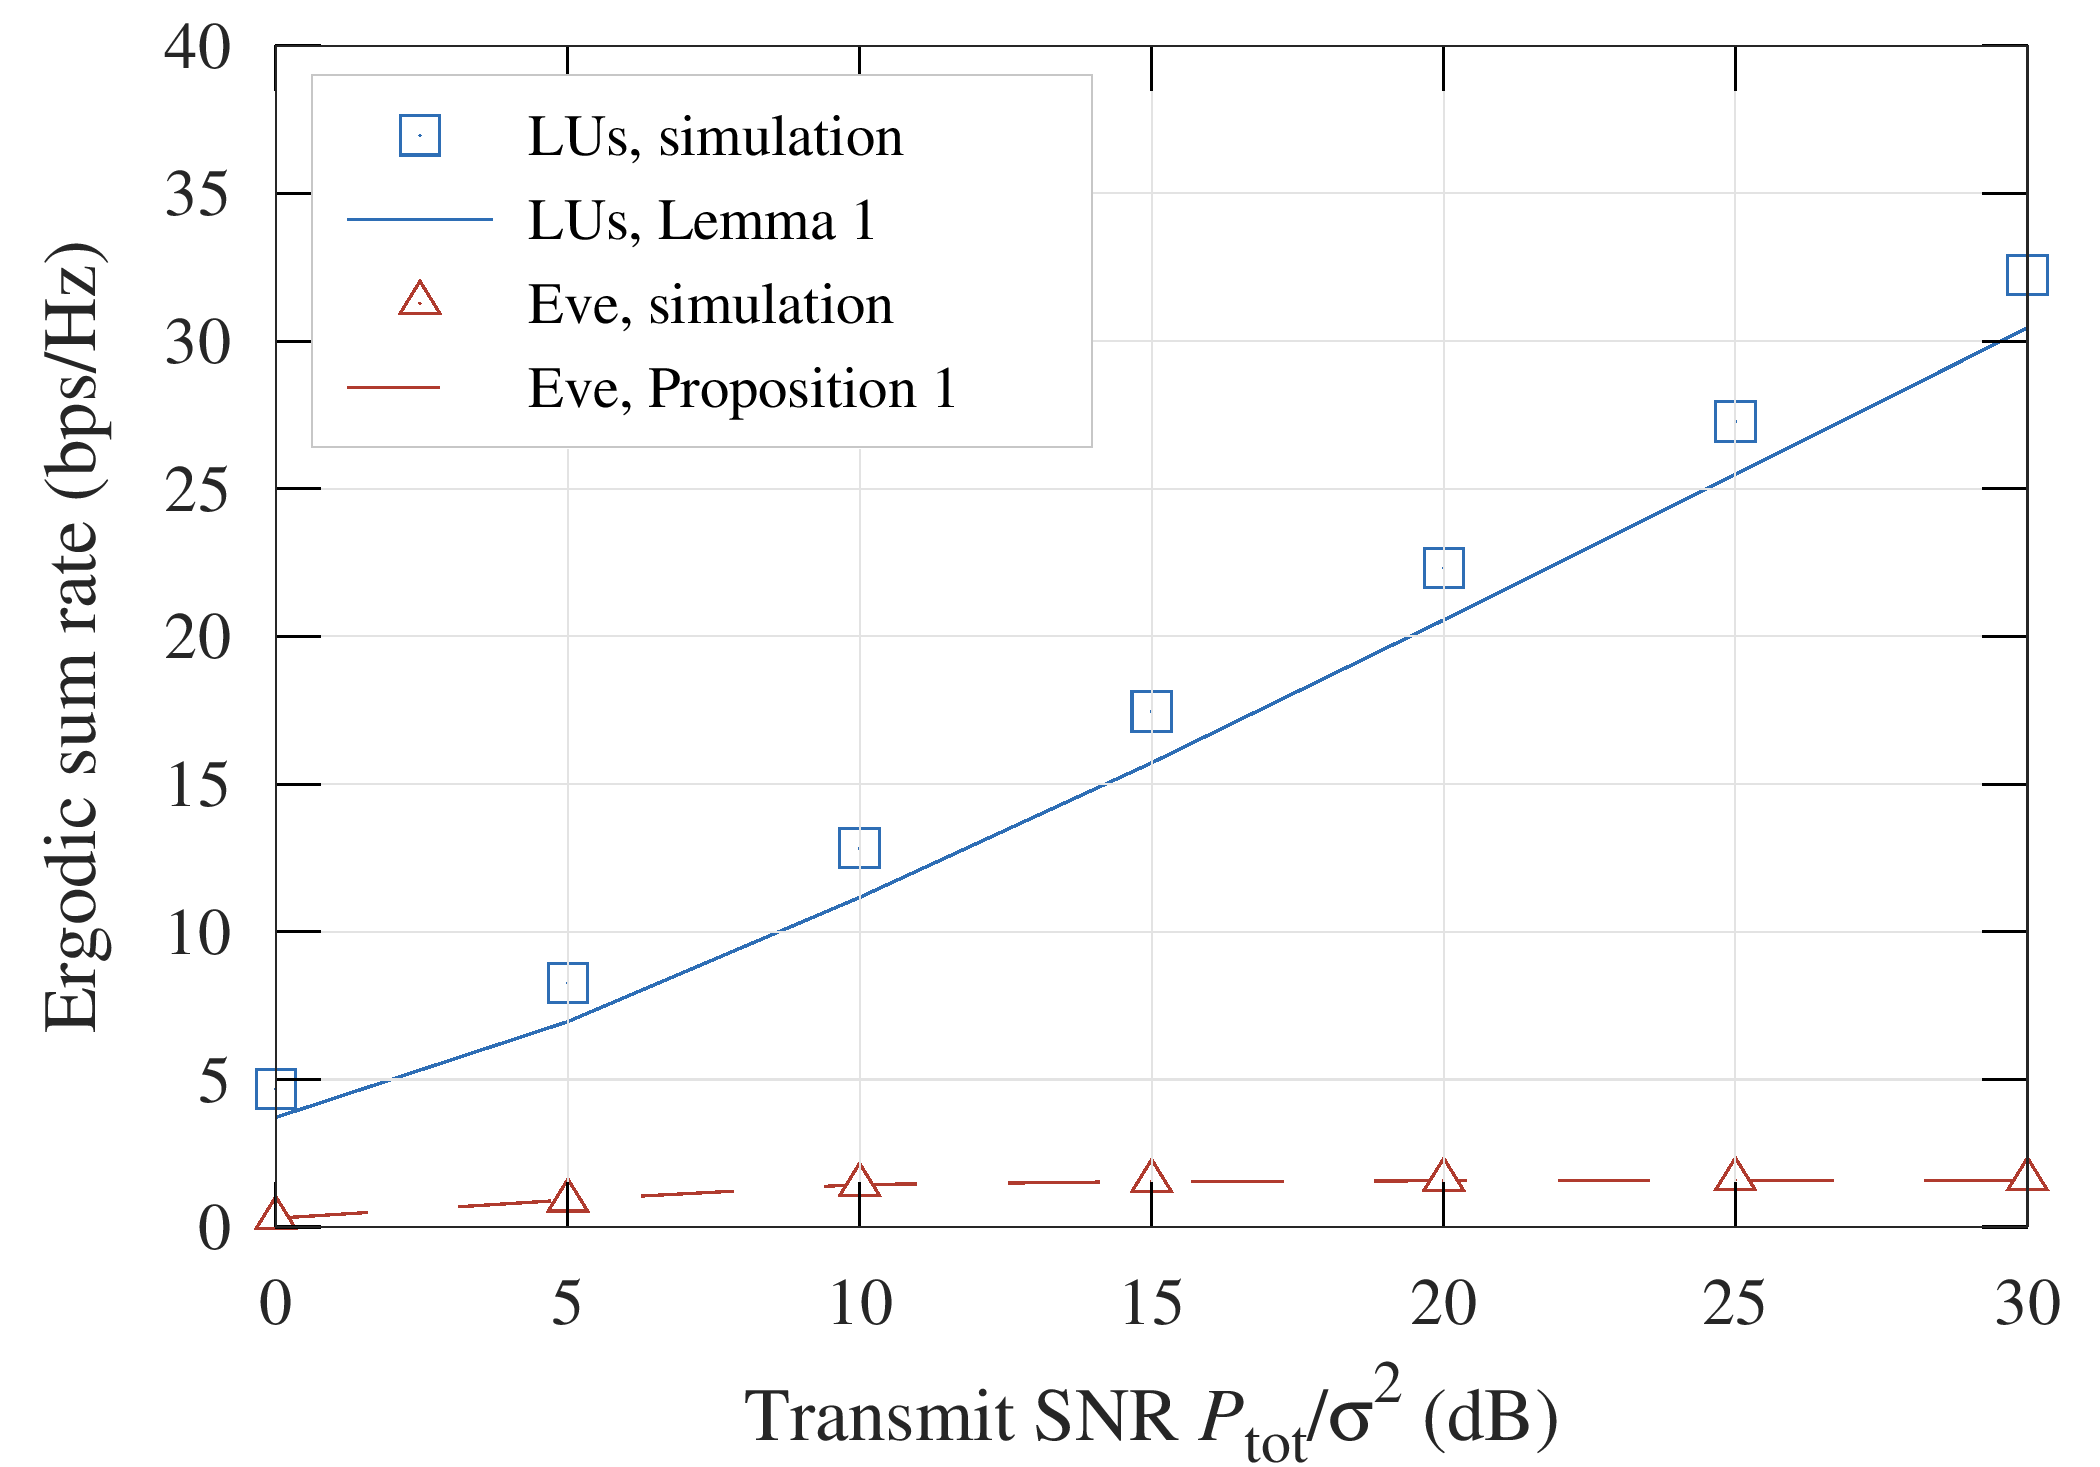
\includegraphics[width=\columnwidth]{fig3a_accuracy_snr}\label{fig:acc_P}}\hfil
\subfloat[]{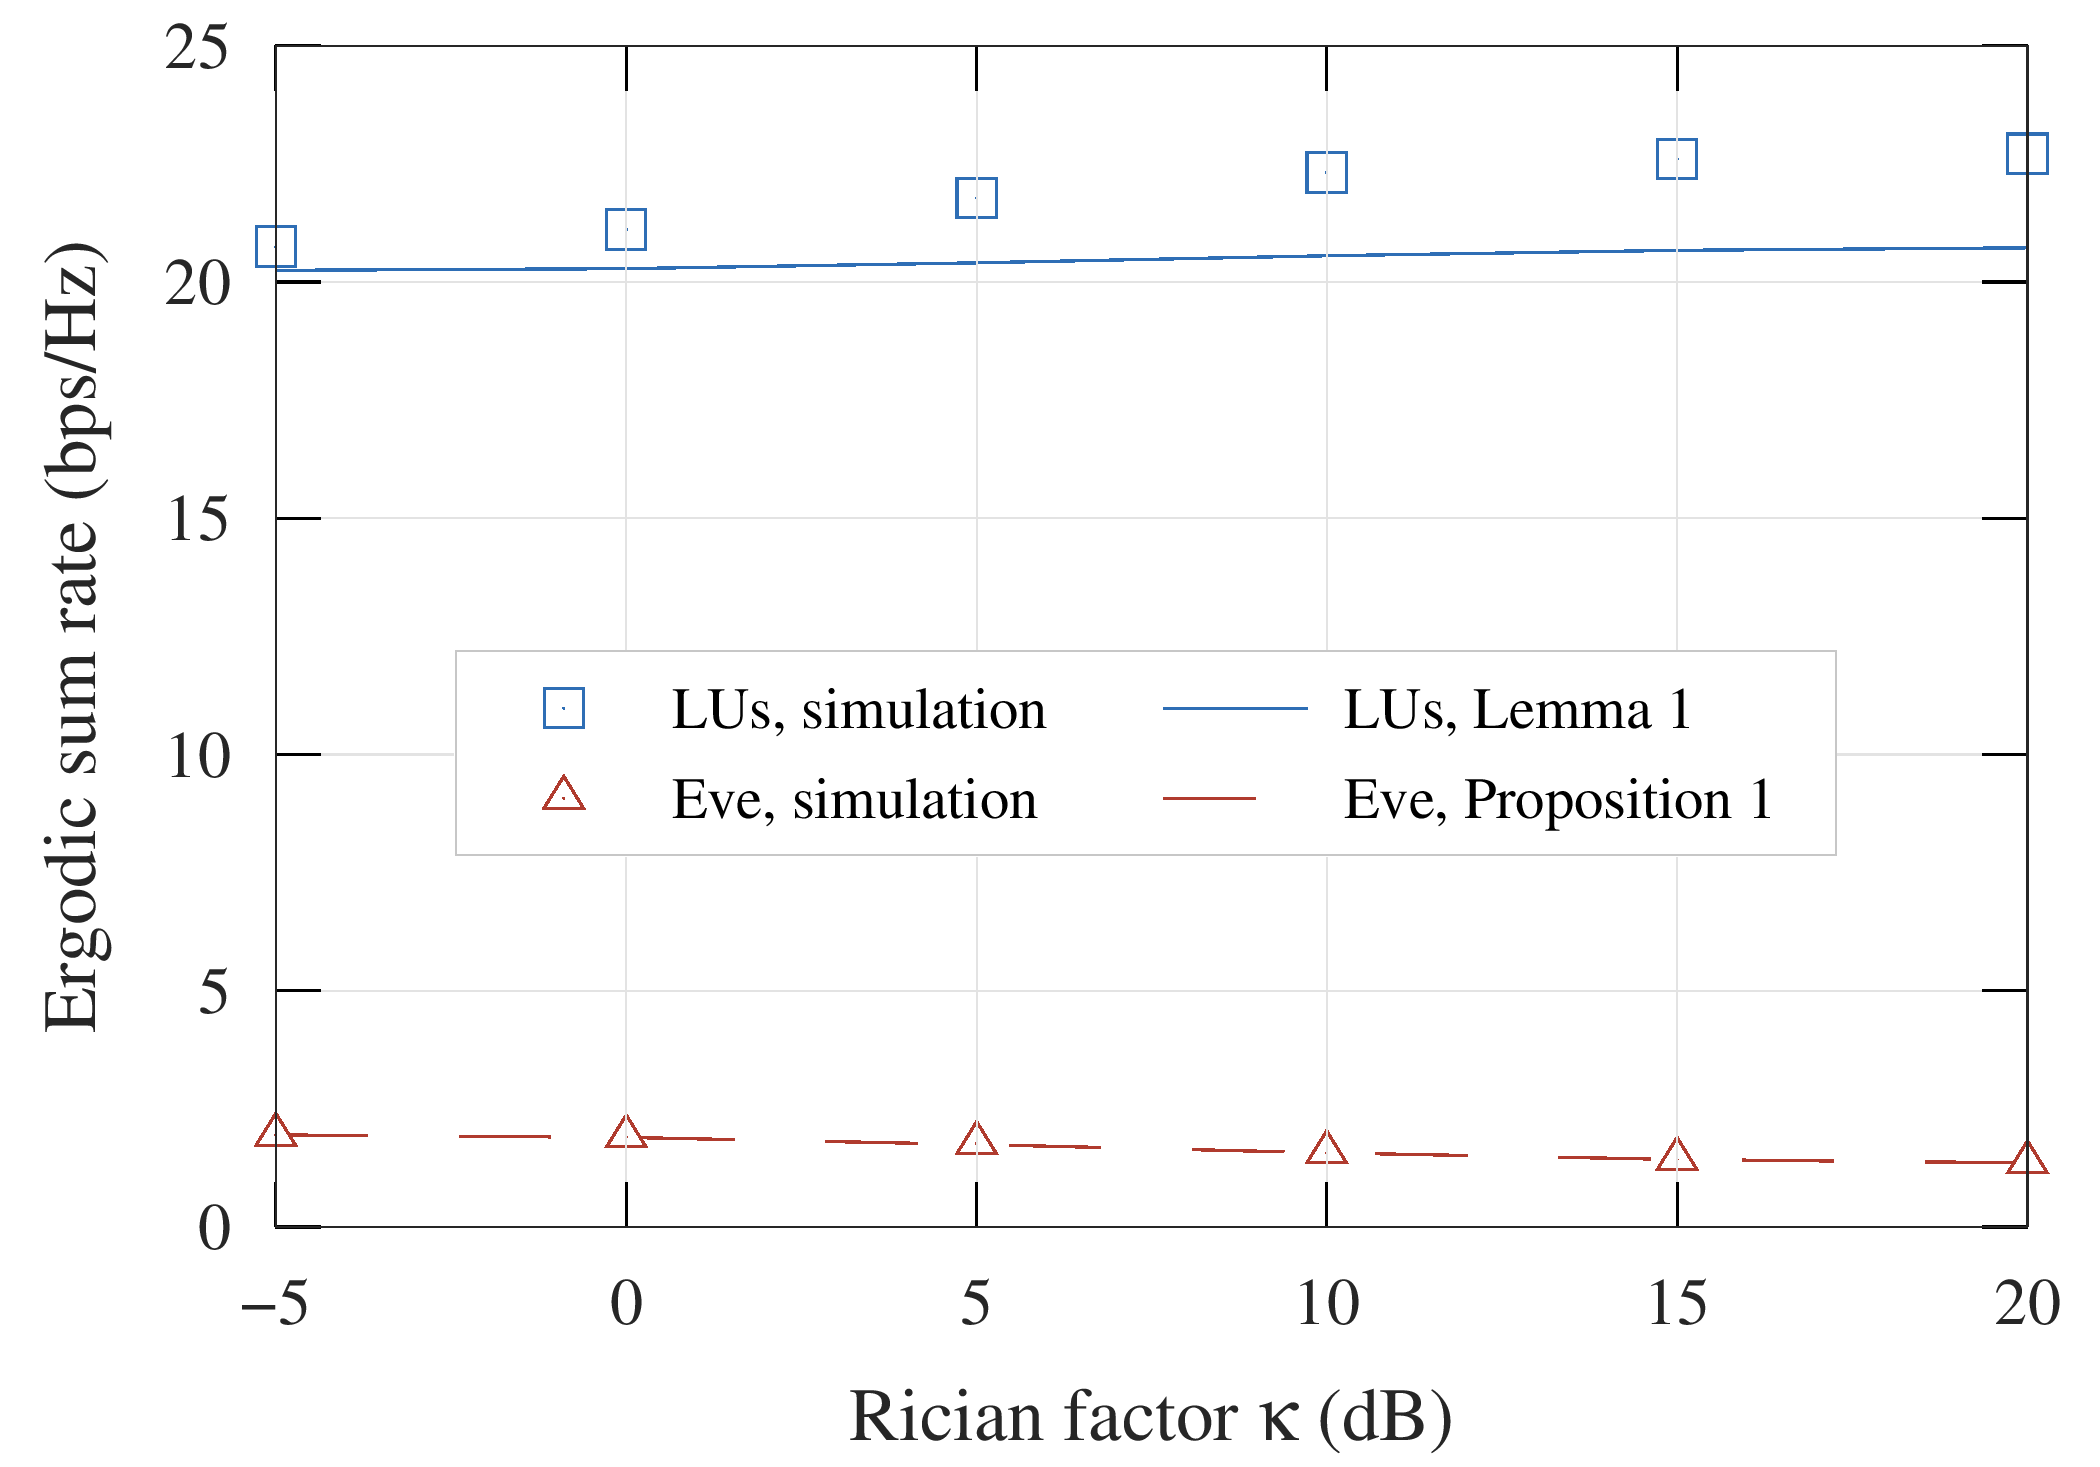
\includegraphics[width=\columnwidth]{fig3b_accuracy_kappa}\label{fig:acc_K}}
\caption{Ergodic sum rates of the LUs and Eve achieved by the proposed design, obtained by Monte Carlo simulations (markers) and by Lemma~\ref{lem:lu} and Proposition~\ref{prop:eve} (lines), versus (a) the transmit SNR $\Ptot/\sigma^2$ and (b) the Rician factor $\kappa=\kappa_m=\kappa_{\mathrm{e}}$.}
\label{fig:acc}
\end{figure*}

Figure~\ref{fig:acc} compares the approximate and Monte Carlo rates at the configurations selected by Algorithm~\ref{alg:ao}. Over the tested SNRs and Rician factors, the largest absolute differences between the approximate and simulated wiretap sum rates are $0.052$ and $0.013$~bit/s/Hz, respectively. These comparisons support the approximation in the tested configurations; they do not establish a bound for arbitrary positions or channel statistics. Lemma~\ref{lem:lu} underestimates the simulated LU sum rate, with a larger discrepancy as the LoS component becomes stronger. Its derivation combines Jensen's inequality with a central-Wishart replacement, whose inverse-moment expression is exact for Rayleigh channels but is generally approximate for Rician channels. Consequently, the resulting ESSR is a surrogate objective rather than a certified lower bound on the true ESSR. At $20$~dB, the proposed configuration has a Monte Carlo ESSR of $20.75$~bit/s/Hz and a surrogate value of $18.98$~bit/s/Hz. Approximation errors can change the ranking of close designs; the reported comparisons therefore use the exact-SINR Monte Carlo rates.

\subsection{Convergence Behavior of Algorithm~\ref{alg:ao}}\label{sec:sim_conv}

\begin{figure}[t]
\centering
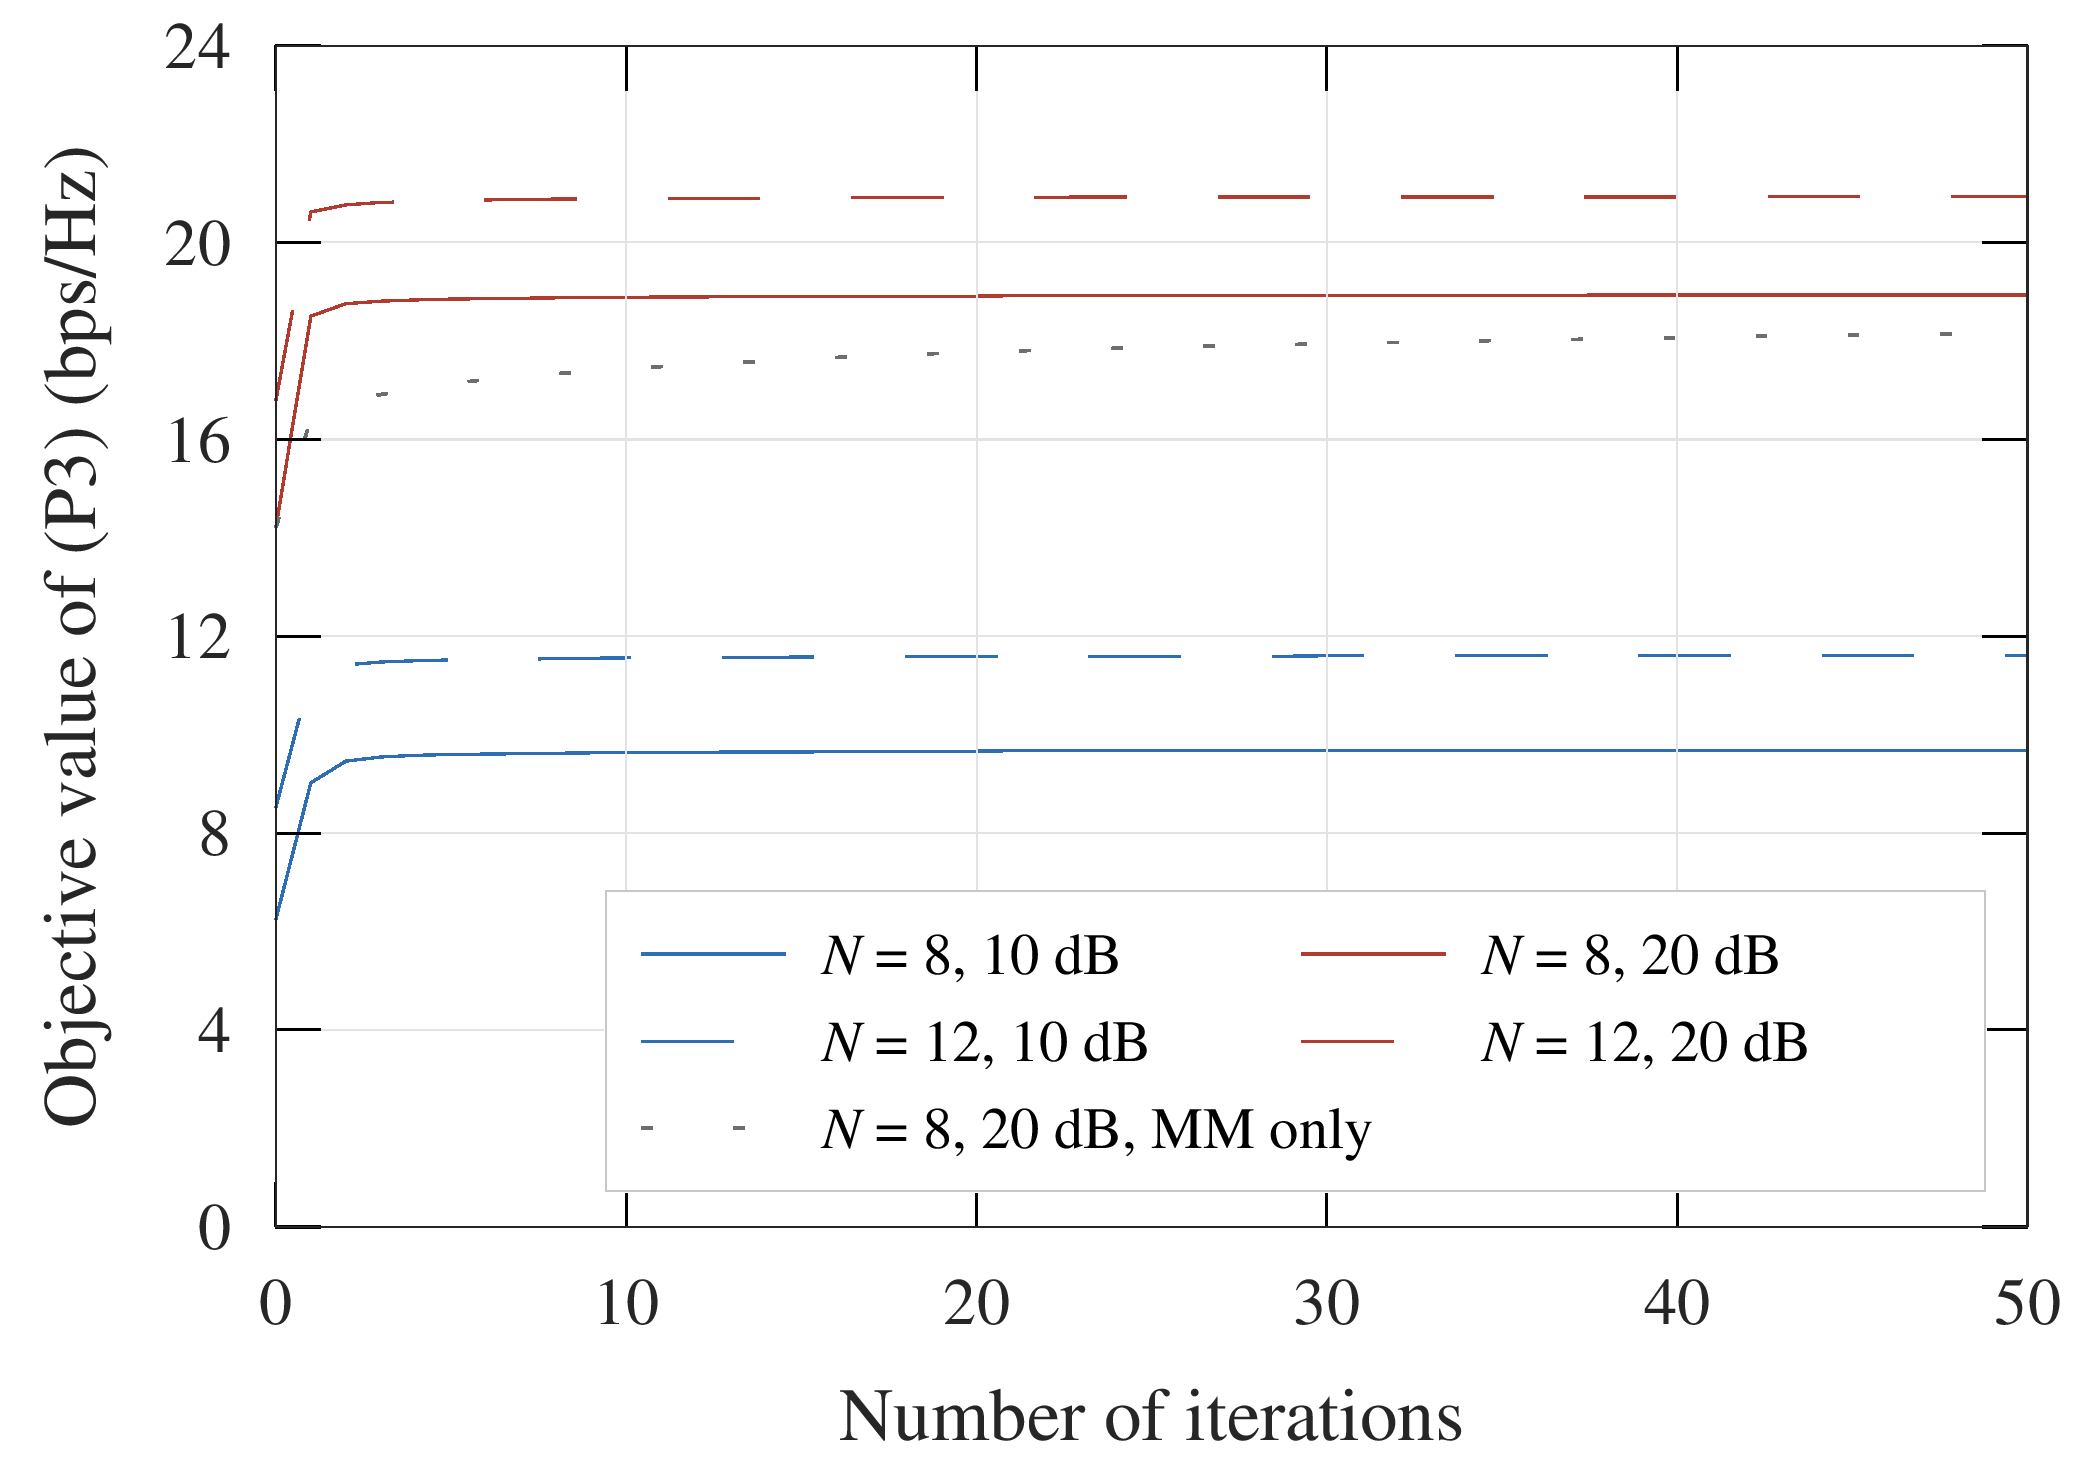
\includegraphics[width=\columnwidth]{fig4_convergence}
\caption{Convergence behavior of Algorithm~\ref{alg:ao} for different numbers of MAs $N$ and transmit SNRs $\Ptot/\sigma^2$, averaged over $100$ AoD realizations (UPA initialization). ``MM only'': without the global search in Stage~1.}
\label{fig:conv}
\end{figure}

Figure~\ref{fig:conv} reports the objective of (P3), with the outer stopping test disabled to retain $50$ iterations. Every stored trajectory is nondecreasing, consistent with the acceptance tests for the position and power updates. The averaged curves are close to their final values after approximately $15$ iterations: their remaining increases are between $0.024$ and $0.034$~bit/s/Hz. This observation does not imply that every realization meets the default stopping test within $15$ iterations. The average stopping indices are $16.31$ and $13.02$ for $N=8$ at $10$ and $20$~dB, and $15.87$ and $12.51$ for $N=12$; some realizations reach the $50$-iteration limit. The feasible-grid stage examines positions beyond the neighborhood accessible to a local MM update. It therefore provides a higher initial improvement in these experiments, while the MM-only variant attains a lower objective. A finite spatial grid does not certify the best continuous attraction region, and monotonic objective convergence does not by itself establish stationarity.

\subsection{ESSR and AN Power Versus Transmit SNR}

\begin{figure*}[t]
\centering
\subfloat[]{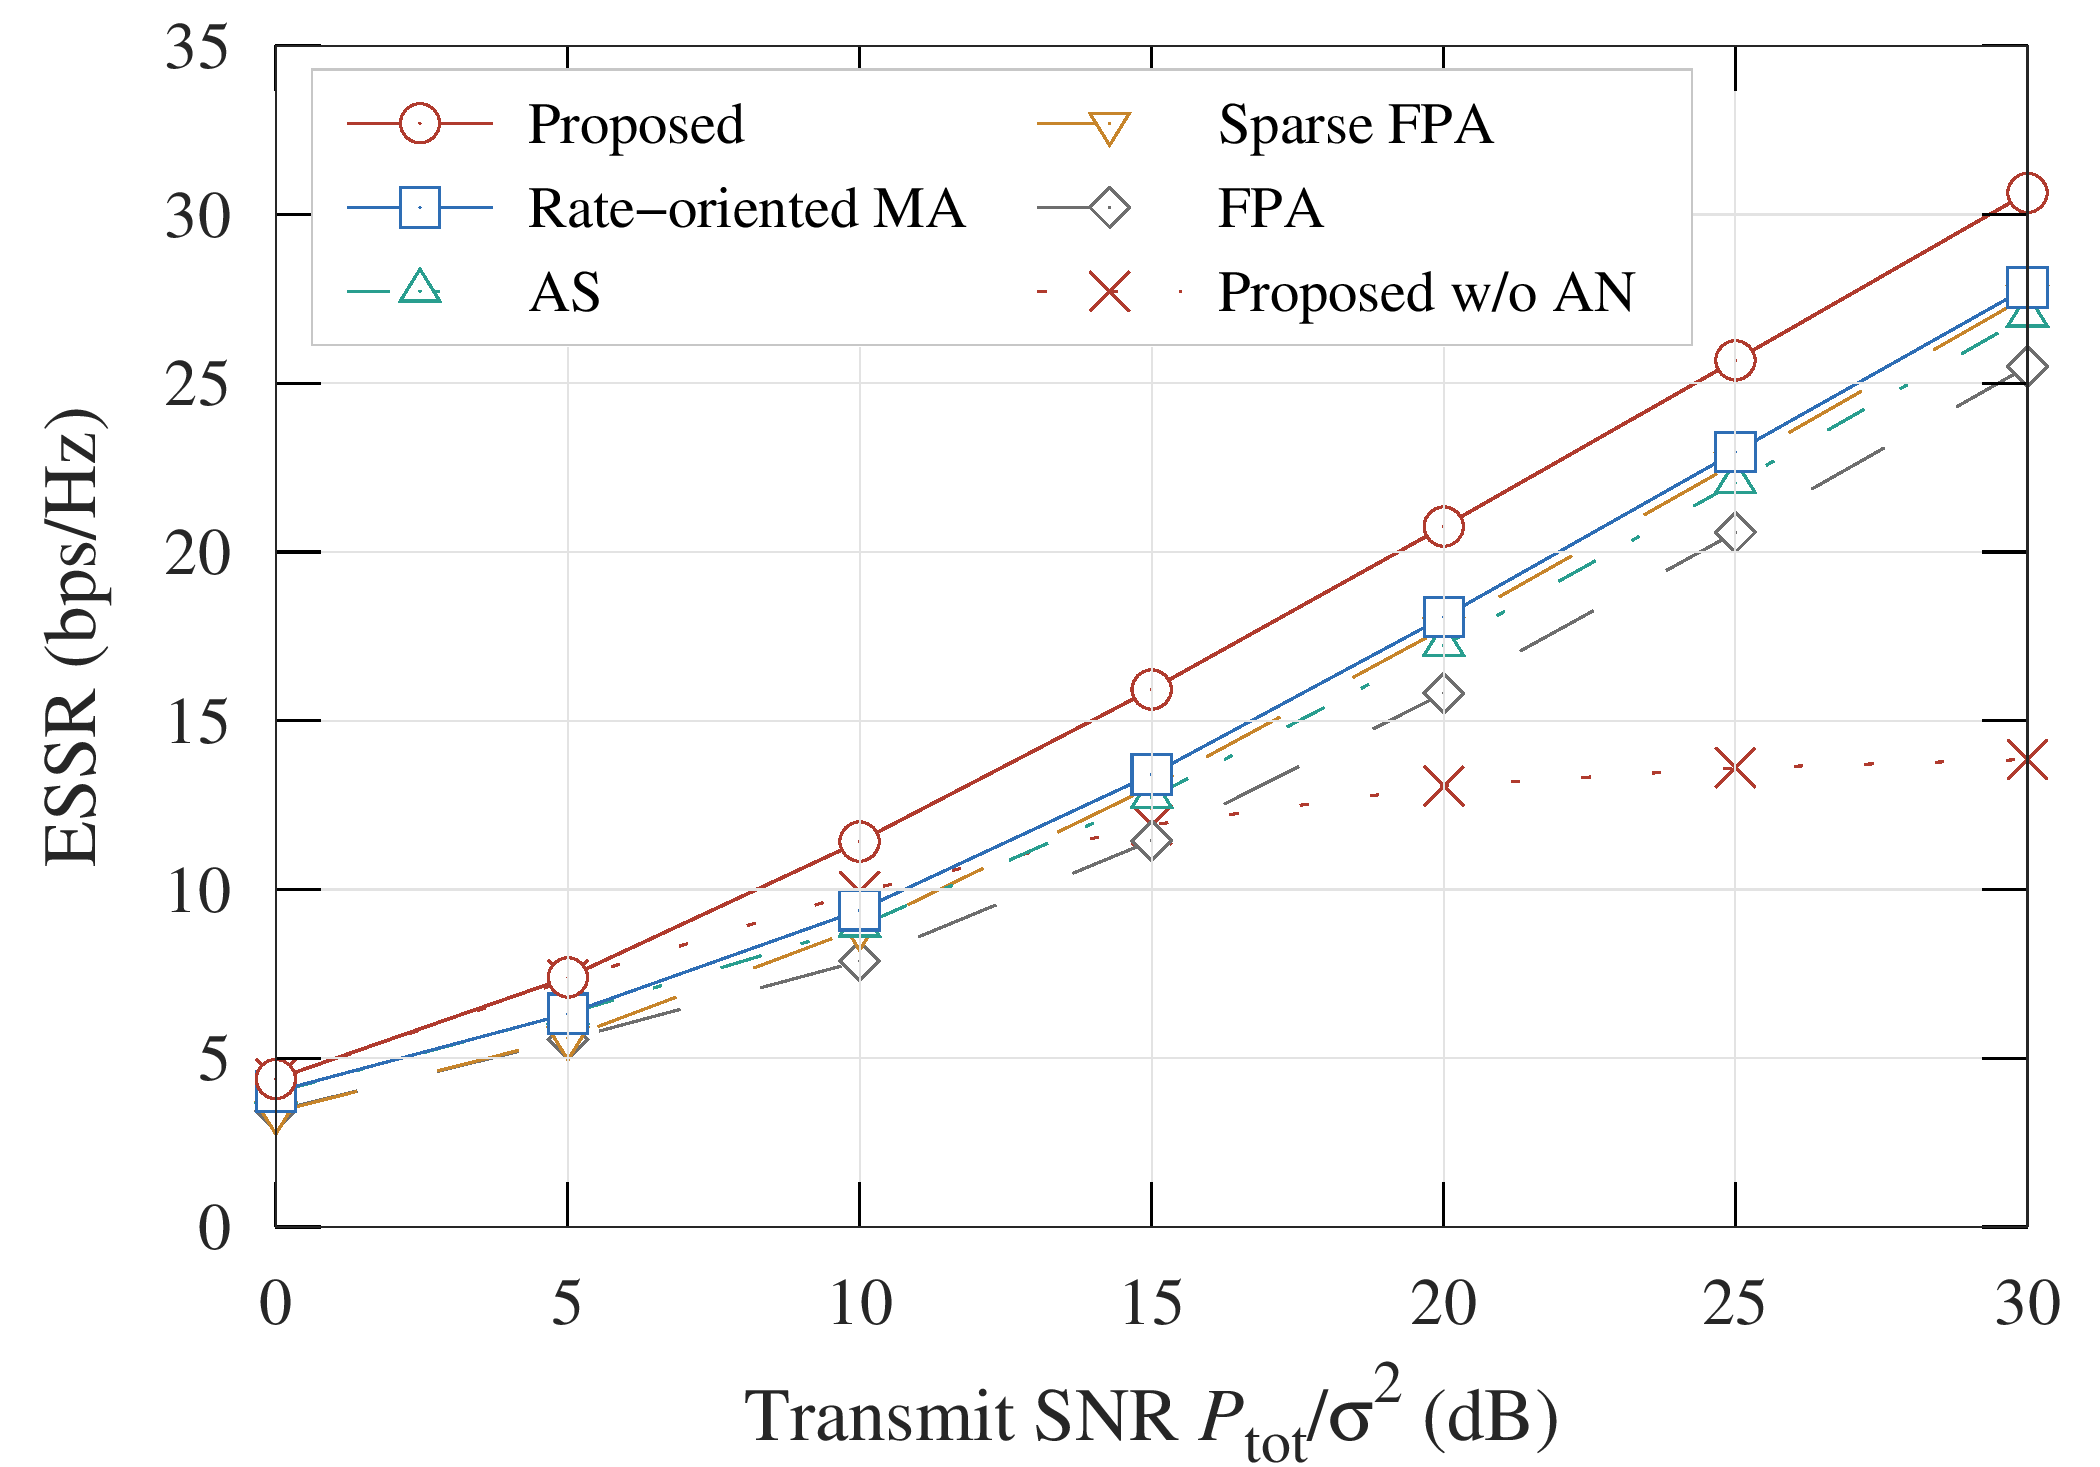
\includegraphics[width=\columnwidth]{fig5a_essr_snr}\label{fig:snr_essr}}\hfil
\subfloat[]{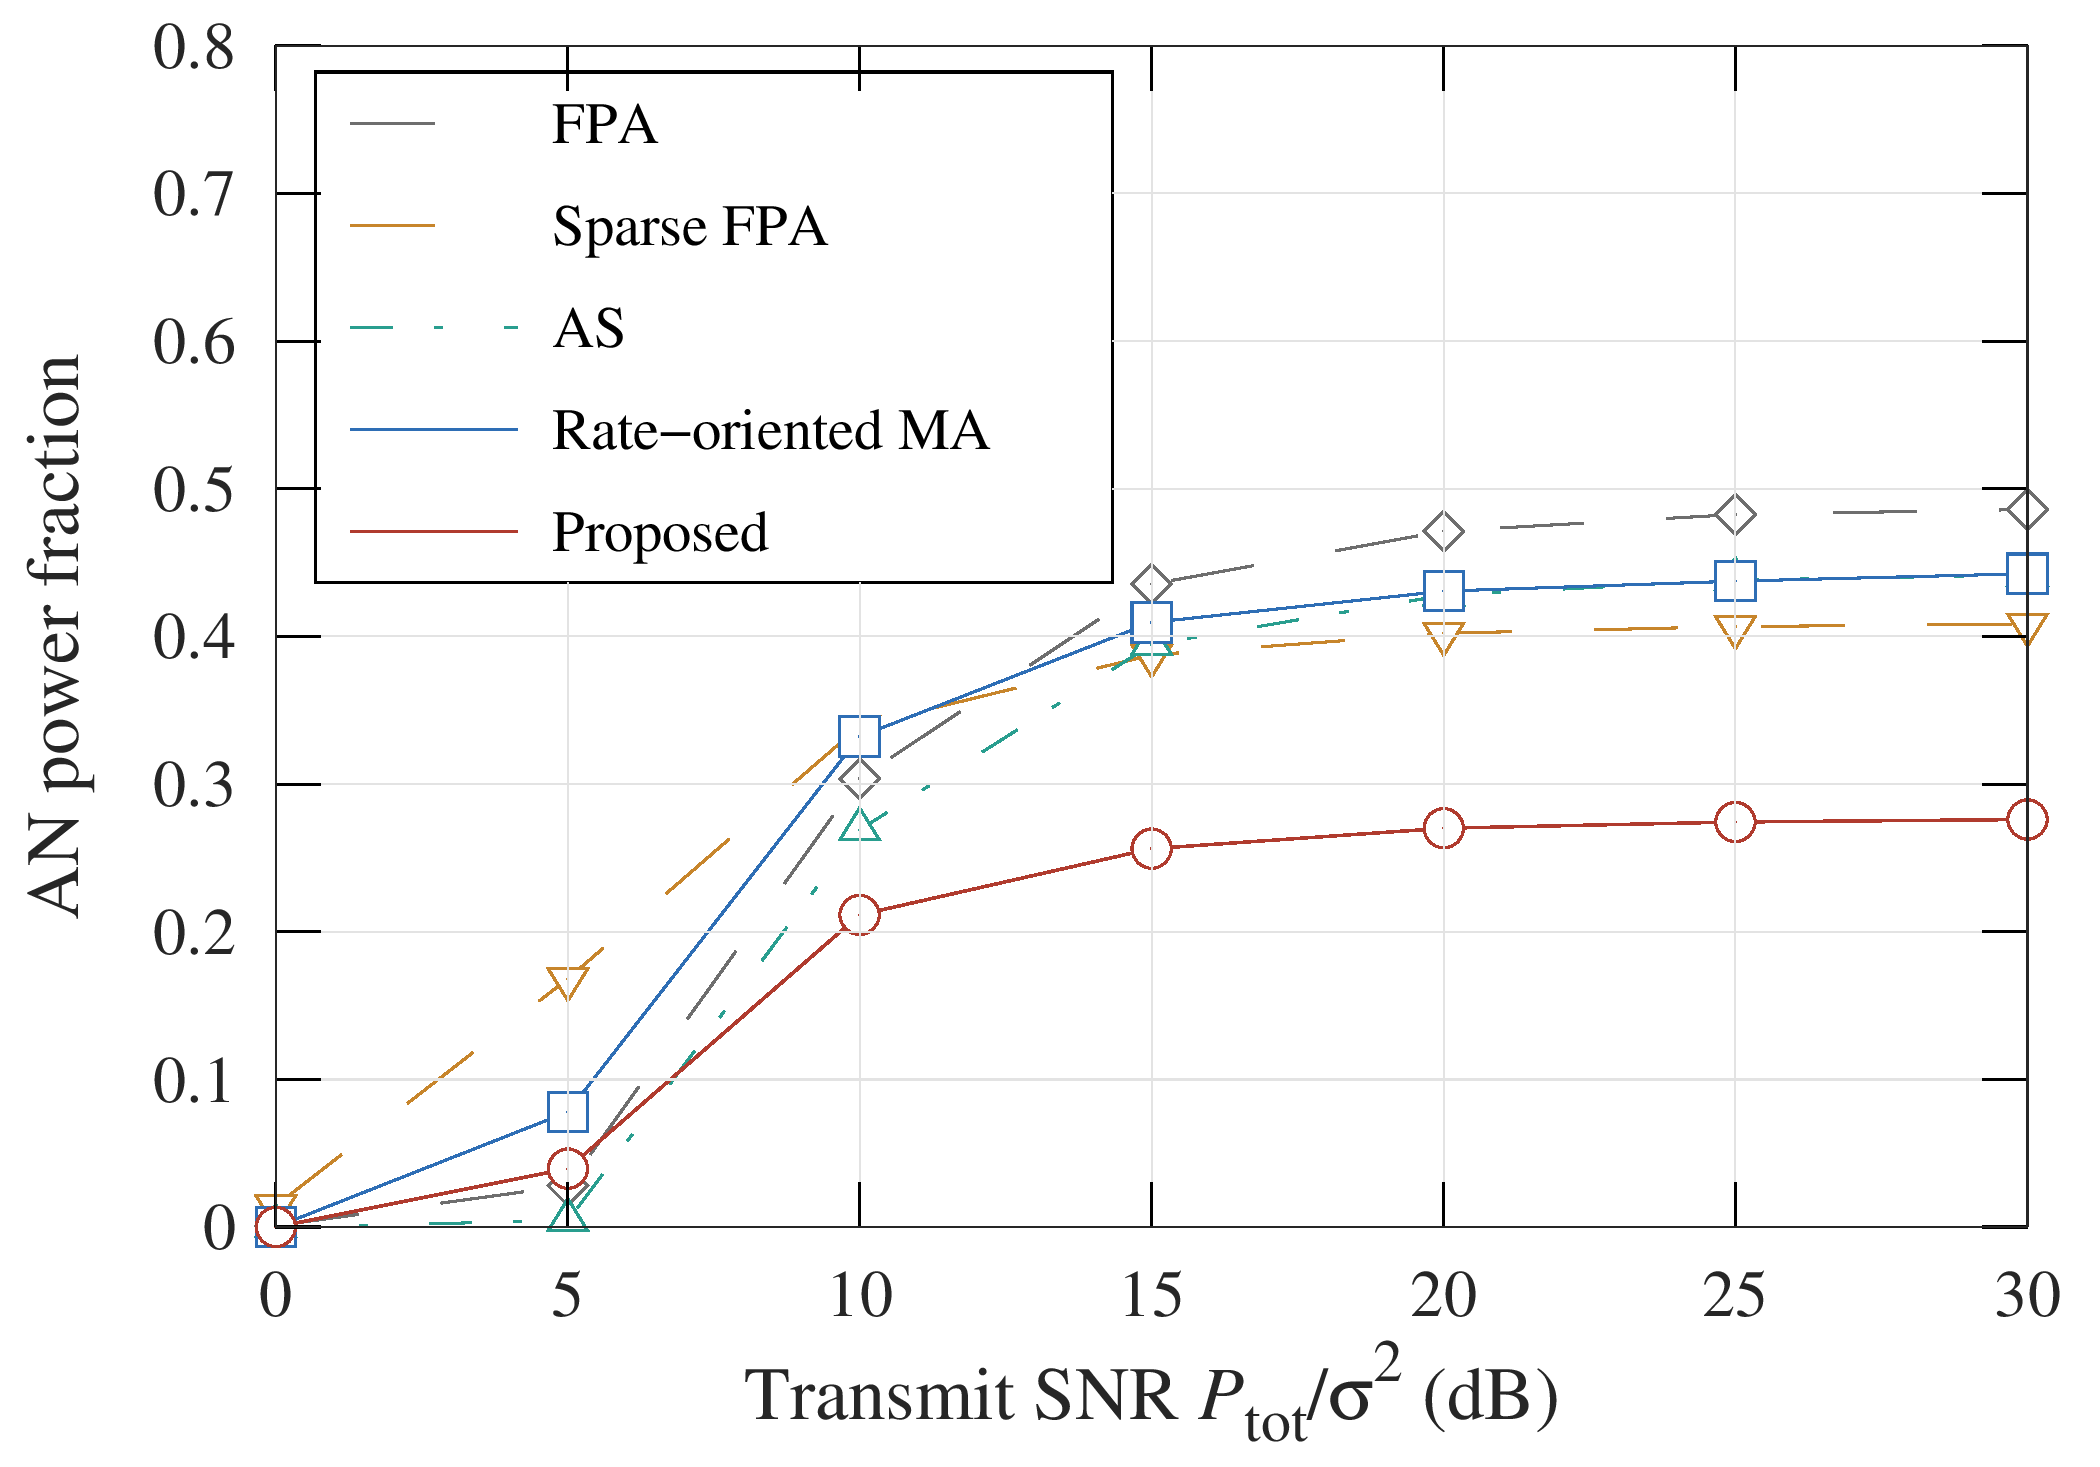
\includegraphics[width=\columnwidth]{fig5b_an_fraction}\label{fig:snr_an}}
\caption{Performance versus the transmit SNR $\Ptot/\sigma^2$: (a) ESSR; (b) optimized AN power fraction $(N-M)q/\Ptot$.}
\label{fig:snr}
\end{figure*}

Figure~\ref{fig:snr}(a) compares the exact-SINR Monte Carlo ESSRs. At $20$~dB, the proposed, rate-oriented, and compact-FPA designs achieve $20.75$, $18.08$, and $15.82$~bit/s/Hz, respectively. The proposed gain is $14.8\%$ over the rate-oriented design and $31.2\%$ over the compact FPA. The rate-oriented objective improves the legitimate-channel geometry through $\eta_m(\bt)$, whereas the secrecy objective also accounts for the leakage coefficients $c_m(\bt)$ and the AN coefficient $d(\bt)$. Position changes can trade these quantities against one another; the formulation does not require every user's leakage to decrease at every iteration. The sparse FPA achieves $17.75$~bit/s/Hz at the same aperture, showing that aperture alone does not reproduce the gain of the adaptive positions in this setting. The compact AS candidates provide a different, discretely constrained set of spatial configurations. At high SNR, the simulated absolute gains change slowly, consistent with the constant-offset comparison in Remark~\ref{rem:highsnr} under its stated assumptions. With $q=0$, the worst-case Eve model yields a secrecy-rate ceiling because the desired and leakage signal powers both scale with the transmit power~\cite{Goel2008}.

Figure~\ref{fig:snr}(b) reports the AN power selected by the surrogate optimization, with each resulting design evaluated as in Fig.~\ref{fig:snr}(a). At $20$~dB, the proposed AN fraction is $0.270$, compared with $0.471$ for the compact FPA and $0.431$ for the rate-oriented MA. Thus, the proposed design allocates approximately $42.7\%$ less power to AN than the compact FPA at this SNR. In Proposition~\ref{prop:eve}, the wiretap rate decreases when the leakage coefficient falls or the effective AN denominator increases. Spatial control therefore changes the tradeoff between confidential-signal power and AN power. The observed fractions level off at high SNR, consistent with~\eqref{eq:alphastar} within the assumptions of Remark~\ref{rem:highsnr}. These fractions are selected by the approximate objective and are not certified minimizers of AN power for a prescribed true ESSR.

\subsection{Impact of the Region Size and the Number of MAs}\label{sec:sim_reg}

\begin{figure*}[t]
\centering
\subfloat[]{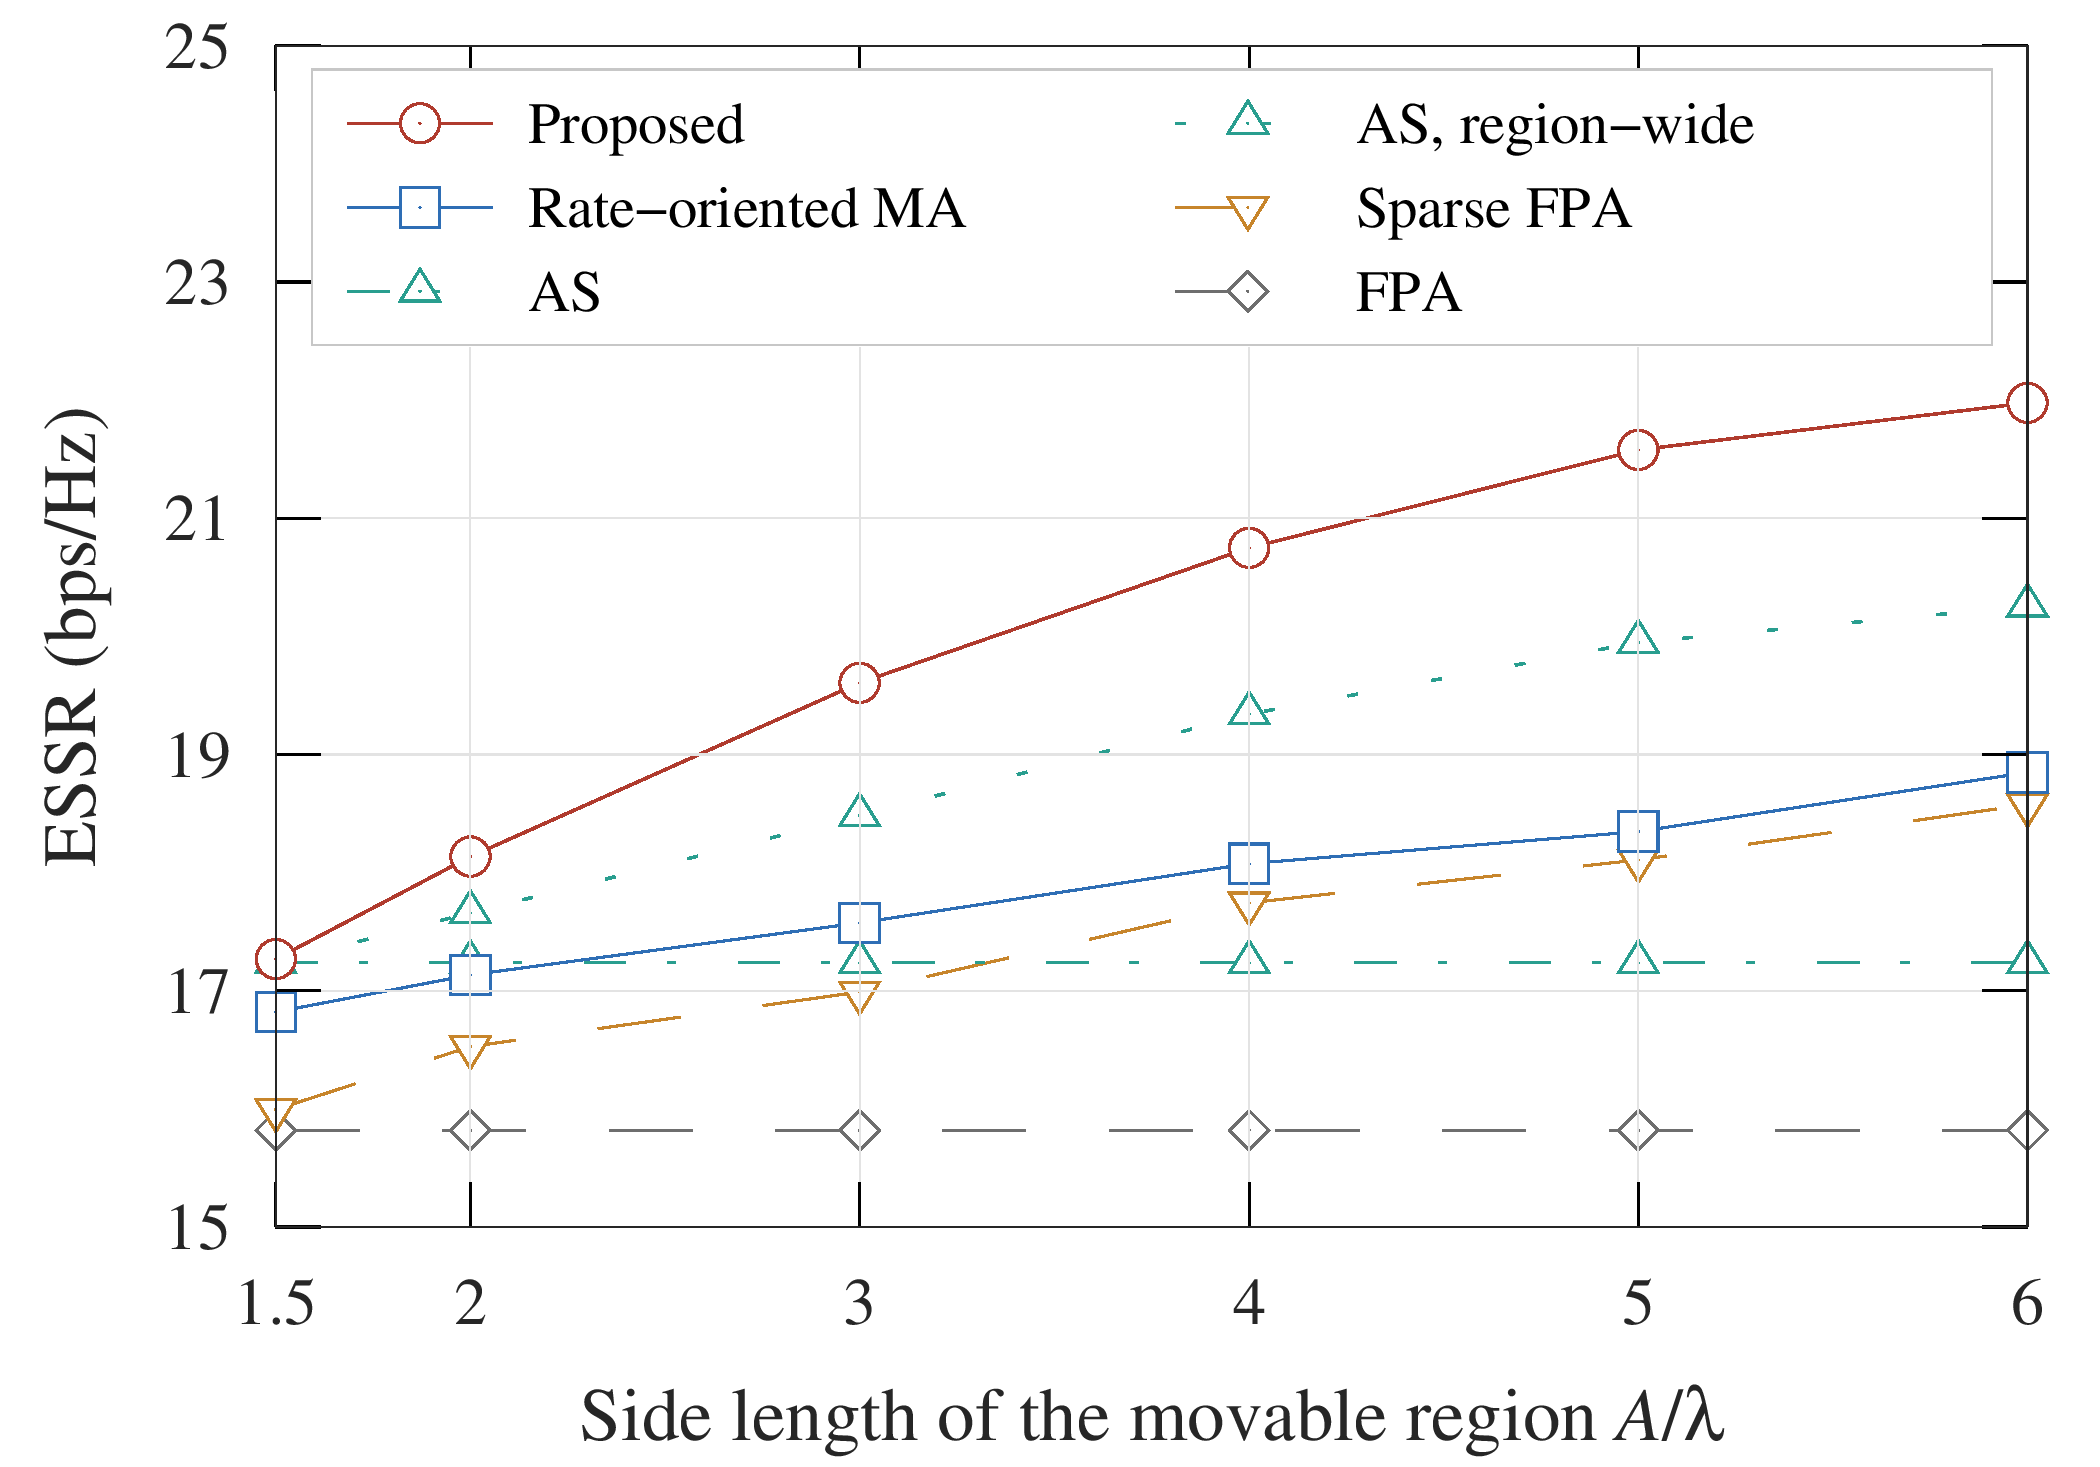
\includegraphics[width=\columnwidth]{fig6a_essr_region}\label{fig:region_A}}\hfil
\subfloat[]{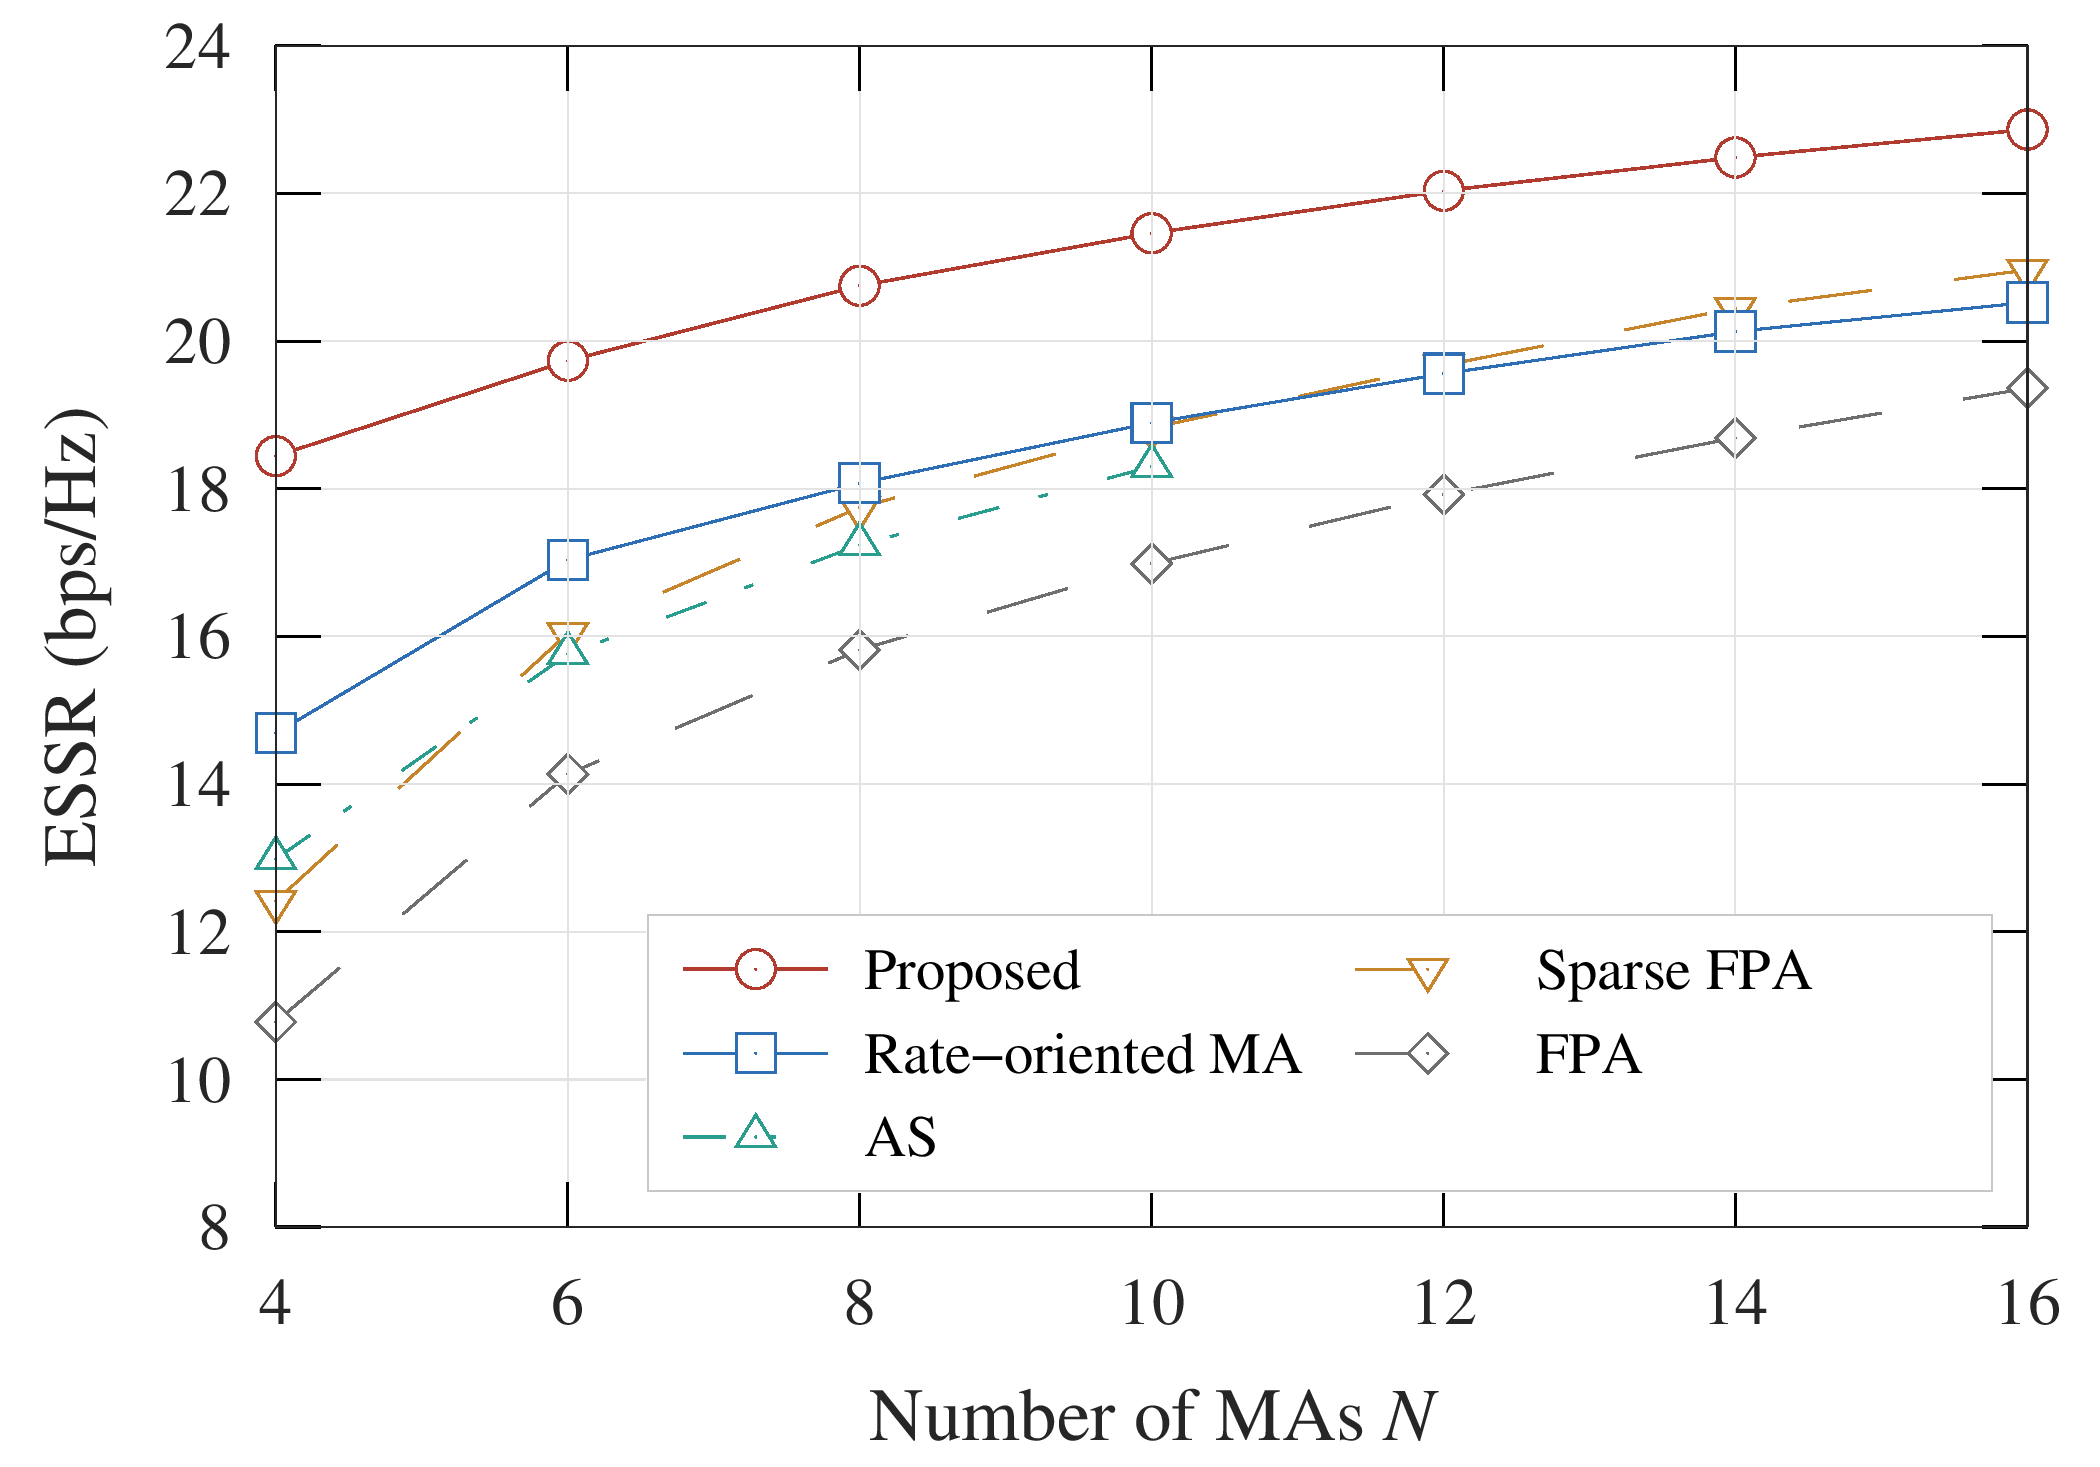
\includegraphics[width=\columnwidth]{fig6b_essr_antennas}\label{fig:region_N}}
\caption{ESSR versus (a) the side length $A$ of the movable region and (b) the number of MAs $N$.}
\label{fig:region}
\end{figure*}

Figure~\ref{fig:region}(a) varies $A$ while retaining $N=8$, $M=3$, and $\Dmin=\lambda/2$. It also includes AS with $16$ candidates on a $4\times4$ UPA spanning $\mathcal C$. A larger region expands the phase differences available for controlling the weighted LoS Gram matrix and its correlation with Eve. The secrecy-aware optimizer can therefore trade legitimate-channel conditioning against leakage suppression and AN reception. The rate-oriented design uses the expanded region only through its LU-rate objective, while the sparse FPA samples a fixed geometry for each $A$. The proposed ESSR increases from $17.27$ to $21.98$~bit/s/Hz over $A/\lambda=1.5$ to $6$ in this experiment. The feasible continuous-position set expands with $A$, but a finite-start algorithm need not produce a monotone curve for every realization. AS with region-wide candidates also benefits from its larger candidate aperture; its comparison with the proposed design concerns continuous versus discrete positioning and $N$ active elements versus $2N$ physical candidate elements. At $A=1.5\lambda$, the compact and region-wide candidate UPAs coincide.

Figure~\ref{fig:region}(b) varies $N$ at $M=3$ and $A=4\lambda$. AS is evaluated only for $N\le10$ because the number of candidate subsets grows as $\binom{2N}{N}$. Increasing $N$ improves the legitimate-channel array gain and enlarges the null space available for AN. The compact FPA aperture also increases with $N$, so this comparison changes both the number of elements and its angular response. In this setting, four optimized MAs achieve $18.44$~bit/s/Hz, exceeding the $17.92$~bit/s/Hz of a compact FPA with $12$ antennas. Eight optimized MAs achieve $20.75$~bit/s/Hz, compared with $20.52$~bit/s/Hz for the rate-oriented design with $16$ MAs. These comparisons identify attainable average rates for the specified geometry rather than a universal antenna-count reduction. For the sparse FPA, increasing $N$ reduces the horizontal element spacing at fixed aperture, changing its sidelobe and grating-lobe structure. This effect can improve separation from Eve without establishing uniform sidelobe suppression for every AoD.

\subsection{Impact of the Coordinate-Angle Offset}\label{sec:sim_sep}

\begin{figure*}[t]
\centering
\subfloat[]{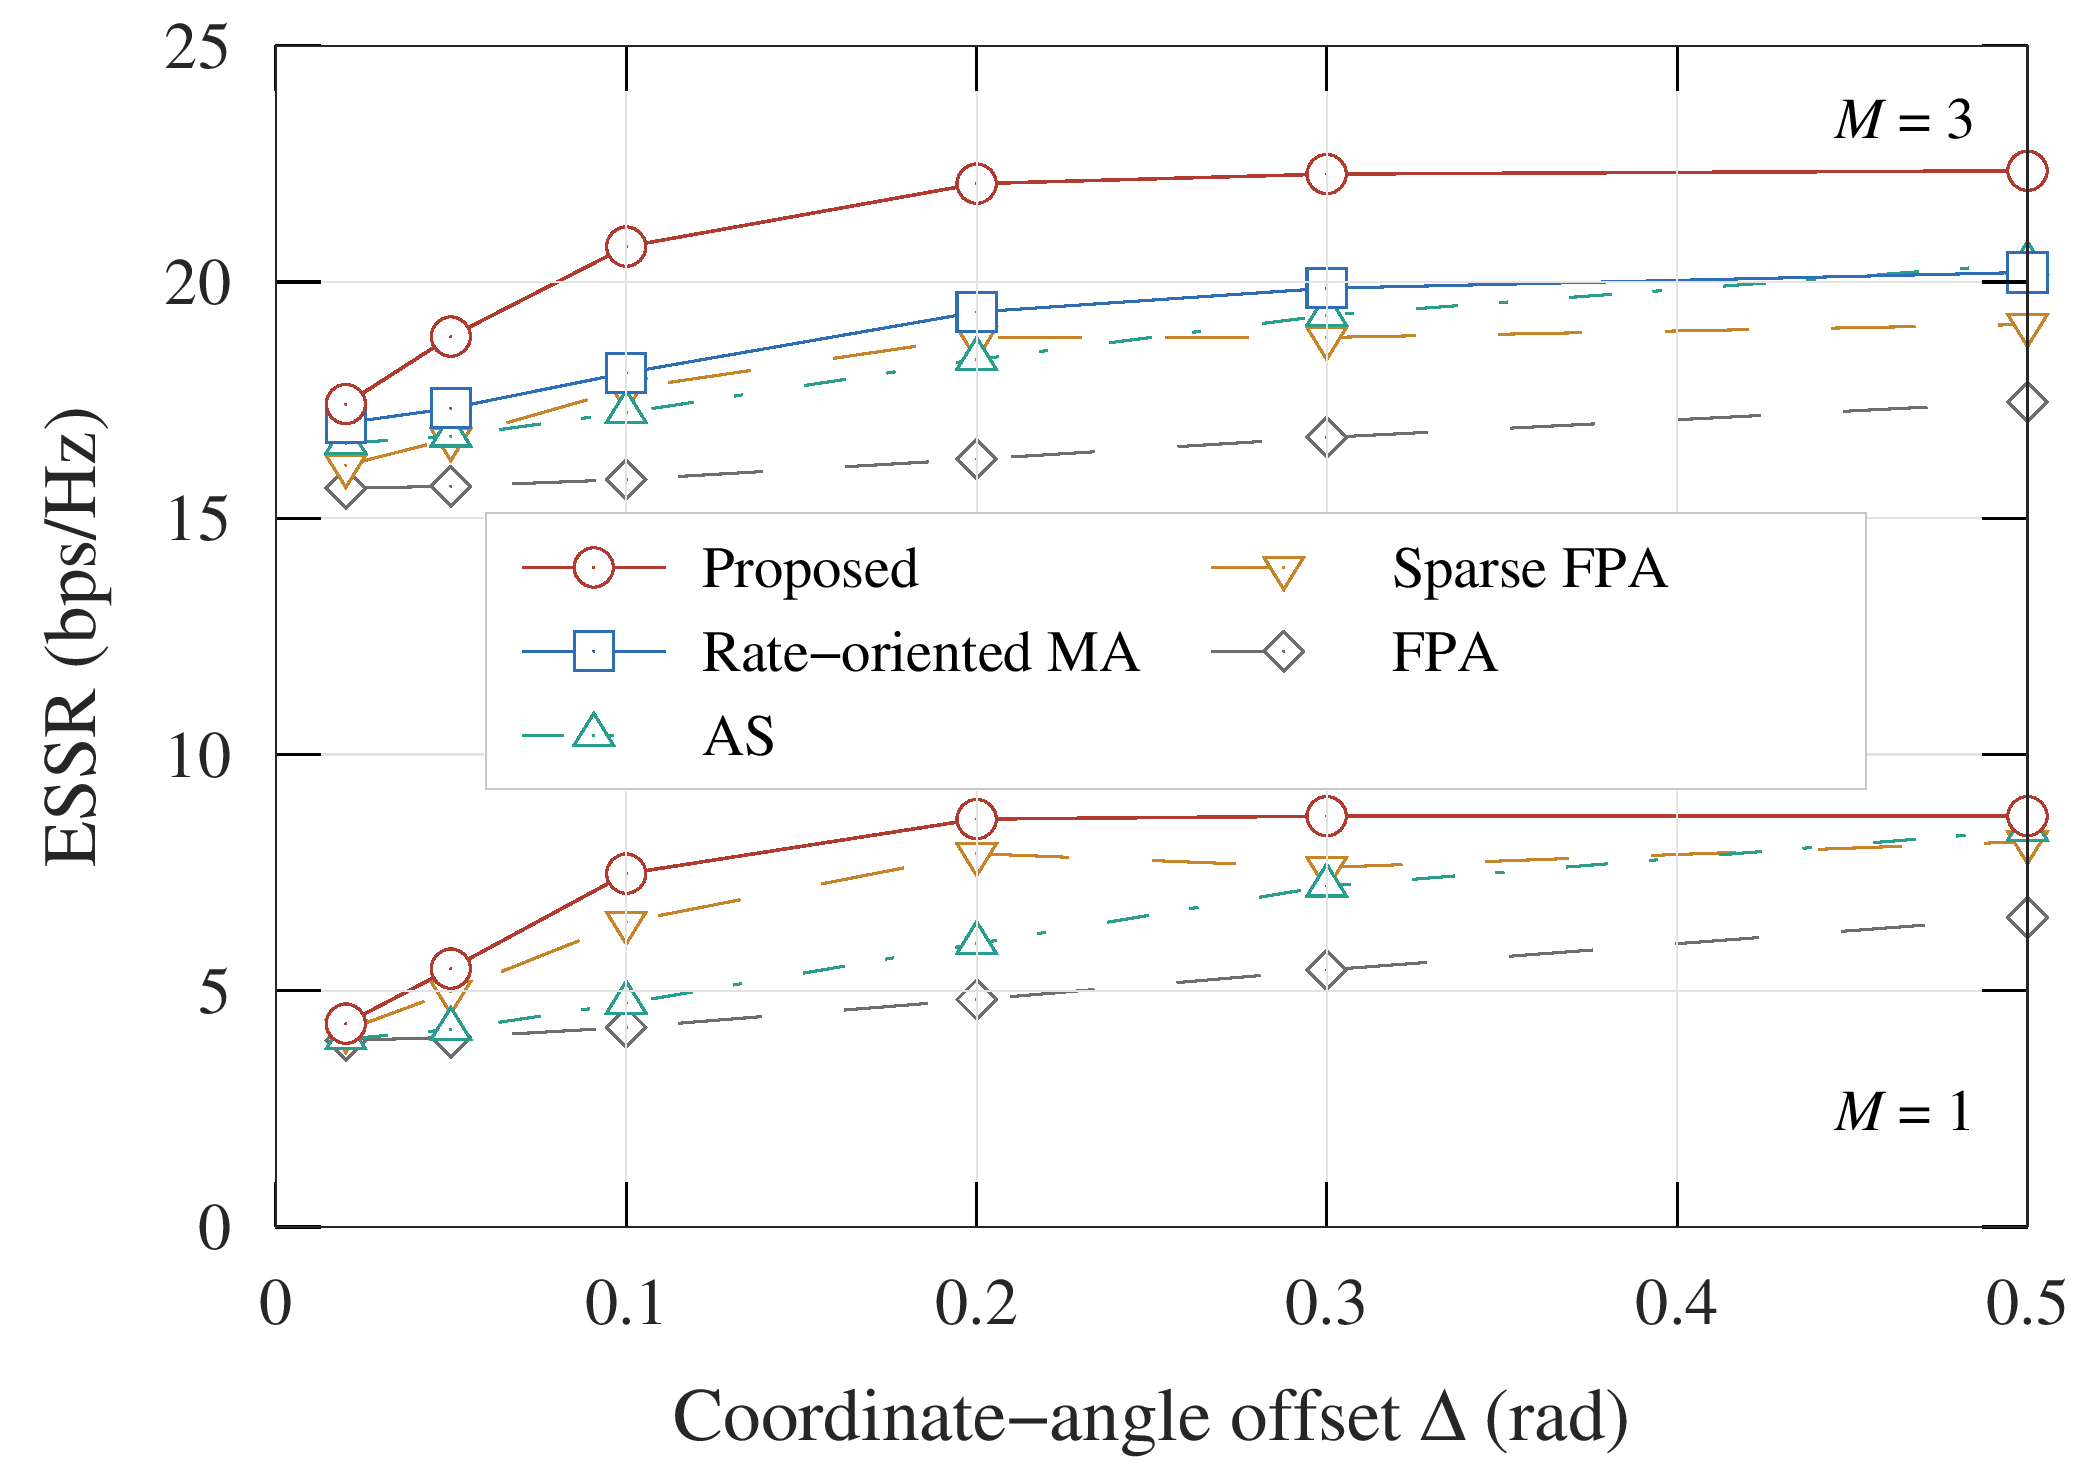
\includegraphics[width=\columnwidth]{fig7a_essr_offset}\label{fig:offset}}\hfil
\subfloat[]{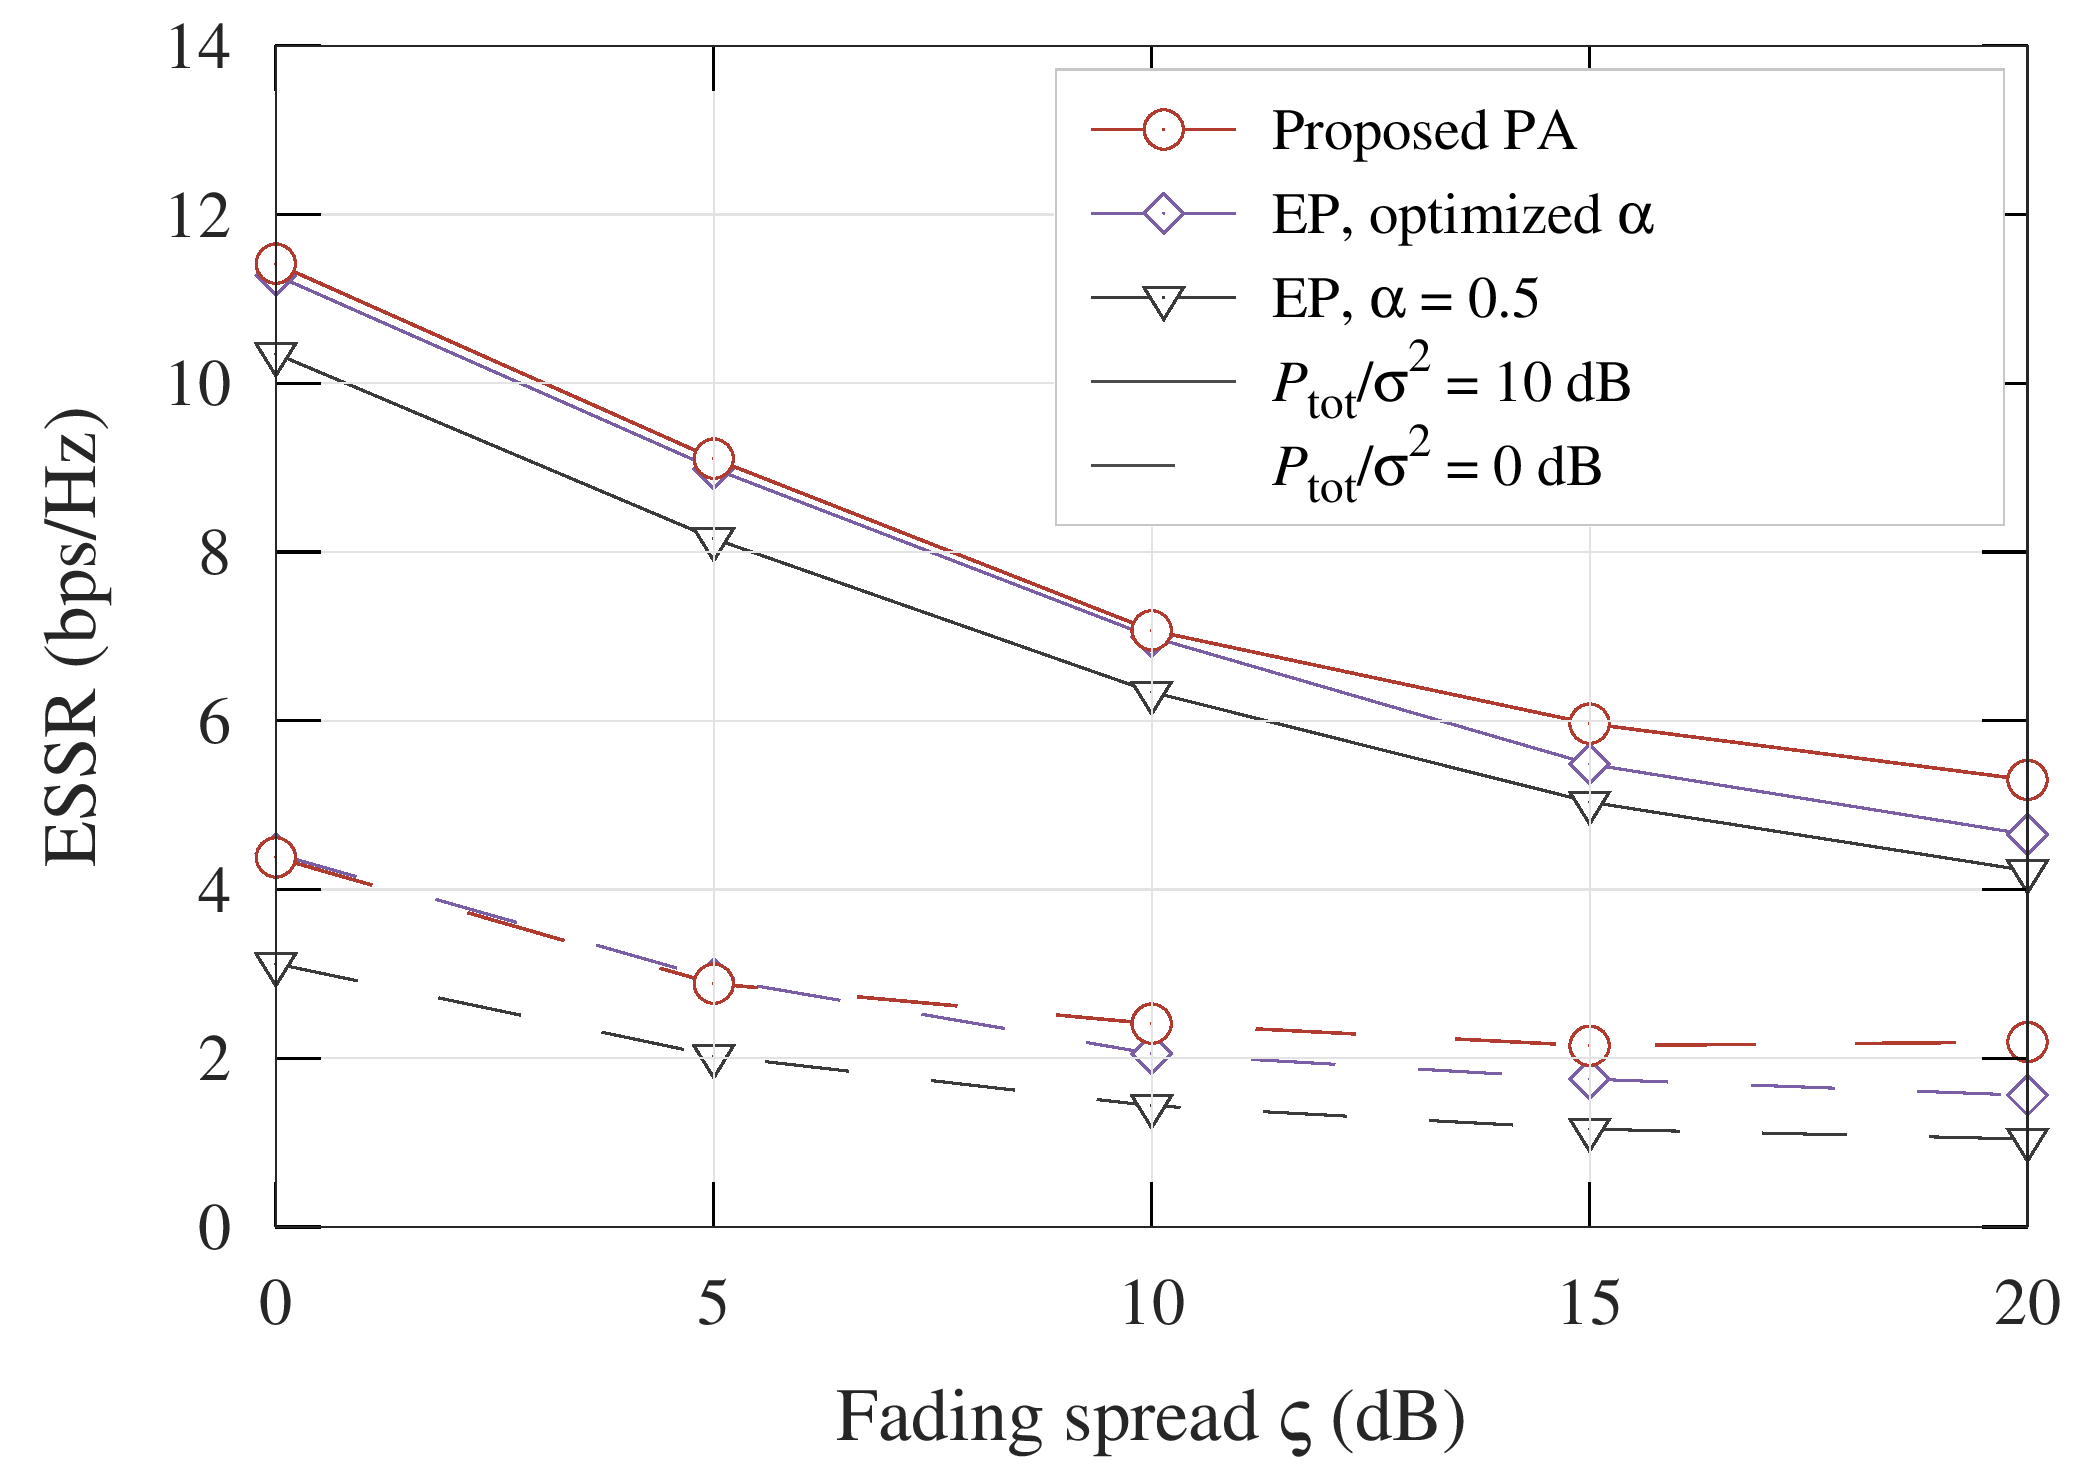
\includegraphics[width=\columnwidth]{fig7b_pa_spread}\label{fig:pa_spread}}
\caption{(a) ESSR versus the coordinate-angle offset $\Delta$ between Eve and LU~$1$ for $M=3$ and $M=1$. (b) ESSR of the proposed power allocation (PA) and two equal-power (EP) benchmarks versus the fading spread $\varsigma$.}
\label{fig:sep_pa}
\end{figure*}

Figure~\ref{fig:sep_pa}(a) varies the coordinate-angle offset $\Delta$ between Eve and LU~$1$. This parameter is the Euclidean offset in the elevation--azimuth coordinates used in Section~\ref{sec:sim_setup}; the corresponding physical separation also depends on the nominal direction. For $M=3$, the proposed and rate-oriented ESSRs are close at $\Delta=0.02$~rad, since the finite aperture limits the phase differences between nearly aligned LoS components. Their gap grows at intermediate offsets and narrows when the rate-oriented positions already provide sufficient separation. For $M=1$, the LU's marginal ergodic rate is independent of position, so the rate-oriented implementation retains the compact UPA. Secrecy-aware positioning still changes the LU--Eve LoS correlation and hence the approximate leakage and AN terms. At $\Delta=0.1$~rad, the proposed single-user ESSR is $7.48$~bit/s/Hz, compared with $4.22$~bit/s/Hz for the compact FPA and $6.45$~bit/s/Hz for the sparse FPA. These rates use exact-SINR evaluation and do not require the finite-Rician moment approximations to satisfy an exact complementary-projection identity.

\subsection{Benefit of the Long-Term Power Allocation}\label{sec:sim_pa}

Figure~\ref{fig:sep_pa}(b) compares the proposed long-term power allocation with two EP benchmarks. The proposed design combines the fixed-AN-power secrecy water-filling solution in Proposition~\ref{prop:wf} with the finite AN-power search. The EP benchmarks use $p_m=\alpha\Ptot/M$ and $q=(1-\alpha)\Ptot/(N-M)$, where $\alpha$ is selected by a finite one-dimensional search, as in the power-splitting approach of~\cite{Zhou2010}, or fixed to $0.5$, as in~\cite{ChenArxiv2026}. Each scheme uses its own power-allocation rule during the position updates, and the EP objective retains $[\cdot]^+$ as discussed in Section~\ref{sec:discussion}. The linear large-scale fading coefficients are $\beta_1=1$, $\beta_2=10^{-\varsigma/20}$, and $\beta_3=10^{-\varsigma/10}$, corresponding to gains of $0$, $-\varsigma/2$, and $-\varsigma$~dB. The fading spread $\varsigma$ is specified in decibels.

At $0$~dB and fading spreads of $0$ and $5$~dB, EP with optimized $\alpha$ attains Monte Carlo ESSRs of $4.425$ and $2.944$~bit/s/Hz, slightly above the proposed PA values of $4.379$ and $2.884$~bit/s/Hz. Its surrogate objectives are lower in both cases. The power-allocation optimum for fixed positions therefore does not imply dominance in the true ESSR after finite-start position optimization. At a $20$-dB fading spread, the proposed PA exceeds optimized EP by $40.3\%$, $13.9\%$, and $0.78\%$ at SNRs of $0$, $10$, and $20$~dB, respectively. The secrecy water-filling rule assigns no power when a user's surrogate legitimate gain does not exceed its effective leakage gain, and reallocates power among the remaining users. This adaptation is useful when the effective gains differ substantially. The smaller measured gains at higher SNRs depend on the tested effective gains and optimized power splits. The equal-user-power expansion in Remark~\ref{rem:highsnr} does not establish that equal user powers are generally asymptotically optimal. EP with $\alpha=0.5$ also expends power on AN at low SNR when the optimized split can select little or no AN. The experiment thus distinguishes the benefit of AN-power selection from that of per-user power adaptation without asserting universal true-ESSR superiority.

\subsection{Robustness of the Secrecy Gain}\label{sec:sim_rob}

We first evaluate the same designs against an Eve that decodes each stream by treating interference as noise (TIN), adding $\sum_{i\ne m}p_i|\bg^{\mathrm{H}}(\bt)\wb_i|^2$ to the denominator of~\eqref{eq:sinre}. For the five AN-enabled designs at SNRs of $10$, $20$, and $30$~dB, the ESSR increases by at most $1.6$~bit/s/Hz. At $20$~dB, the increases are $0.49$ and $1.47$~bit/s/Hz for the proposed and rate-oriented designs. The smaller increase for the proposed design is consistent with lower received inter-user leakage, which also reduces the interference protecting a stream against a TIN receiver. For the no-AN design at $30$~dB, the TIN and worst-case ESSRs are $27.14$ and $13.85$~bit/s/Hz, respectively. Inter-user interference can therefore protect the evaluated TIN receiver, whereas the worst-case model excludes that protection. The need for AN at high SNR follows from the specified eavesdropper model and does not establish that every secrecy target requires AN.

We next perturb the Eve direction available to the BS by a coordinate-angle offset $\varepsilon_{\mathrm e}$ in a uniformly random direction, using the construction in Section~\ref{sec:sim_setup}. The designs use the perturbed statistical CSI and the rate evaluations use the true CSI. At $20$~dB, the proposed ESSR decreases from $20.75$ to $20.13$~bit/s/Hz at $\varepsilon_{\mathrm e}=0.05$~rad, a $3.0\%$ reduction, and to $18.73$~bit/s/Hz at $0.1$~rad. It remains above the largest benchmark value, $17.93$~bit/s/Hz, in this experiment. Errors affect the proposed positions as well as the power allocation; the rate-oriented and fixed-position schemes depend on the perturbed Eve CSI only through power allocation, and AS also depends on it through subset selection. Smooth LoS phases explain continuity of the rate evaluation at fixed designs, but do not alone guarantee a small optimization loss or robustness to arbitrary errors. These experiments establish tolerance for the tested offsets rather than a worst-case robust-design guarantee.

{\widowpenalty=10000
Finally, Eve's elevation and azimuth are drawn independently of the LUs from $[-\pi/3,\pi/3]$. For $M=3$, the proposed, rate-oriented, and sparse-FPA ESSRs are $22.30$, $20.23$, and $18.91$~bit/s/Hz, giving proposed gains of $10.3\%$ and $17.9\%$. For $M=1$, AS achieves $8.49$~bit/s/Hz, close to the proposed value of $8.67$~bit/s/Hz. Independent directions reduce the frequency of near alignment, allowing the compact AS candidates to separate Eve from a single LU in more realizations. These averages complement the near-alignment experiment; they do not imply that a large movable aperture is necessary in every individual geometry.\par}


% =============================================================================
\section{Conclusion}\label{sec:conclusion}
% =============================================================================
This paper investigates two-timescale secure transmission for an MA-enabled multiuser downlink with statistical CSI of a passive Eve. A closed-form wiretap-rate approximation characterizes how antenna positions affect information leakage and the AN received by Eve, in addition to the LU ZF gains. The resulting deterministic objective supports an AO method that combines optimal per-user power allocation for fixed AN power, sampled AN-power search, and grid-assisted MM position updates. Feasibility-preserving updates and an acceptance test produce nondecreasing, bounded objective values. The reported simulations show secrecy gains over the rate-oriented MA design, AS, and FPA arrays, including gains with one LU and lower AN-power fractions in the evaluated settings. Extending the model to multiple multi-antenna eavesdroppers and imperfect LU CSI requires new leakage analysis and uncertainty-aware optimization.

% =============================================================================
\appendices
\section{Proof of Lemma~\ref{lem:indep}}\label{app:indep}
% =============================================================================
Let $\mathbf U=[\mathbf u_1,\ldots,\mathbf u_{N-M}]\in\mathbb C^{N\times(N-M)}$ have orthonormal columns spanning the null space of $\bH^{\mathrm{H}}(\bt)$. Then $\PHp=\mathbf U\mathbf U^{\mathrm{H}}$ and $Y=\sum_{i=1}^{N-M}|\mathbf u_i^{\mathrm{H}}\bg(\bt)|^2$. The unit-norm ZF direction $\wb_m$ lies in the column space of $\bH(\bt)$. Thus, $\mathbf Q\triangleq[\wb_m,\mathbf U]\in\mathbb C^{N\times(N-M+1)}$ satisfies $\mathbf Q^{\mathrm{H}}\mathbf Q=\bI_{N-M+1}$.

Since $\gtl$ is independent of $\bH(\bt)$, the conditional distribution induced by~\eqref{eq:g} is proper complex Gaussian with mean $\sqrt{\kappa_{\mathrm{e}}\tilde\beta_{\mathrm{e}}}\,\gb(\bt)$ and covariance $\tilde\beta_{\mathrm{e}}\bI_N$. Conditioned on $\bH(\bt)$, $\mathbf Q^{\mathrm{H}}\bg(\bt)$ is therefore proper complex Gaussian with covariance $\tilde\beta_{\mathrm{e}}\bI_{N-M+1}$. Its entries are conditionally independent, so $X_m=|\wb_m^{\mathrm{H}}\bg(\bt)|^2$ is conditionally independent of $Y$. For a proper scalar $z\sim\CN(\mu,\tilde\beta_{\mathrm{e}})$, the identities $\E\{|z|^2\}=|\mu|^2+\tilde\beta_{\mathrm{e}}$ and $\mathrm{Var}\{|z|^2\}=\tilde\beta_{\mathrm{e}}^2+2|\mu|^2\tilde\beta_{\mathrm{e}}$ yield~\eqref{eq:EX} and~\eqref{eq:EY}, using $\sum_{i=1}^{N-M}|\mathbf u_i^{\mathrm{H}}\gb(\bt)|^2=\bar Y$.

% =============================================================================
\section{Proof of Proposition~\ref{prop:eve}}\label{app:det}
% =============================================================================
We construct approximations for two moments of a noncentral Gaussian matrix and then apply them to~\eqref{eq:Re0}. The following lemma establishes their ranges and their exact limiting cases; it does not provide a finite-parameter error bound.

\begin{lemma}\label{lem:det}
Let $\bF=\Fb+\bW\in\mathbb C^{N\times M}$ with $M<N$, where $\Fb$ is deterministic and the entries of $\bW$ are i.i.d.\ $\CN(0,1)$ random variables. Let $\bb\in\mathbb C^{N\times1}$ be a deterministic vector, and define $\bPhi_{\bF}\triangleq\E\{\bF^{\mathrm{H}}\bF\}=\Fb^{\mathrm{H}}\Fb+N\bI_M$, $\wb_m(\bF)\triangleq\bF(\bF^{\mathrm{H}}\bF)^{-1}\be_m/\|\bF(\bF^{\mathrm{H}}\bF)^{-1}\be_m\|$, and $\mathbf P_{\bF}^\perp\triangleq\bI_N-\bF(\bF^{\mathrm{H}}\bF)^{-1}\bF^{\mathrm{H}}$. Then, we have
\begin{align}
\E\{|\bb^{\mathrm{H}}\wb_m(\bF)|^2\}
&\approx\frac{1}{[\bPhi_{\bF}^{-1}]_{m,m}}
\nonumber\\
&\quad\times\Big(
 \big|[\bPhi_{\bF}^{-1}\Fb^{\mathrm{H}}\bb]_m\big|^2
 +\|\bb\|^2[\bPhi_{\bF}^{-2}]_{m,m}\Big),
\label{eq:lem_c}\\
\E\{\bb^{\mathrm{H}}\mathbf P_{\bF}^{\perp}\bb\}
&\approx\frac{N-M}
 {N-M+N\tr(\bPhi_{\bF}^{-1})}
\nonumber\\
&\quad\times\big(
 \|\bb\|^2-\bb^{\mathrm{H}}\Fb\bPhi_{\bF}^{-1}\Fb^{\mathrm{H}}\bb\big).
\label{eq:lem_d}
\end{align}
Moreover, \eqref{eq:lem_c} and~\eqref{eq:lem_d} are exact for $\Fb=\mathbf 0$, and are asymptotically exact for $\Fb=\varrho\Fb_0$ as $\varrho\to\infty$, where $\Fb_0$ has full column rank. The right-hand sides of~\eqref{eq:lem_c} and~\eqref{eq:lem_d} lie in $[0,\|\bb\|^2]$, as do their left-hand sides.
\end{lemma}

\begin{IEEEproof}
For brevity, let $\bPhi\triangleq\bPhi_{\bF}$. To construct~\eqref{eq:lem_c}, first replace the random inverse $(\bF^{\mathrm{H}}\bF)^{-1}$ in the unnormalized ZF direction by $\bPhi^{-1}$. Then approximate the expectation of the normalized quadratic ratio by the ratio of its numerator and denominator expectations, in the same spirit as~\cite[Lemma~1]{ZhangJSTSP2014}. These are two distinct approximations; neither follows from $\E\{(\bF^{\mathrm{H}}\bF)^{-1}\}=(\E\{\bF^{\mathrm{H}}\bF\})^{-1}$, which does not hold in general. For the deterministic vector $\bPhi^{-1}\be_m$, the required moments are exact because $\E\{\bW\}=\mathbf 0$ and $\E\{\bW\mathbf x\mathbf x^{\mathrm{H}}\bW^{\mathrm{H}}\}=\|\mathbf x\|^2\bI_N$ for any deterministic $\mathbf x$. Hence,
\begin{align}
\E\{|\bb^{\mathrm{H}}\bF\bPhi^{-1}\be_m|^2\}
&=|\bb^{\mathrm{H}}\Fb\bPhi^{-1}\be_m|^2
\nonumber\\
&\quad+\|\bb\|^2\|\bPhi^{-1}\be_m\|^2
\nonumber\\
&=\big|[\bPhi^{-1}\Fb^{\mathrm{H}}\bb]_m\big|^2
\nonumber\\
&\quad+\|\bb\|^2[\bPhi^{-2}]_{m,m},
\label{eq:app1}\\
\E\{\|\bF\bPhi^{-1}\be_m\|^2\}
&=\be_m^{\mathrm{T}}\bPhi^{-1}\bPhi\bPhi^{-1}\be_m
\nonumber\\
&=[\bPhi^{-1}]_{m,m},
\label{eq:app2}
\end{align}
which define the approximation in~\eqref{eq:lem_c}. To construct~\eqref{eq:lem_d}, replacing the random inverse in $\mathbf P_{\bF}\triangleq\bI_N-\mathbf P_{\bF}^{\perp}=\bF(\bF^{\mathrm{H}}\bF)^{-1}\bF^{\mathrm{H}}$ by $\bPhi^{-1}$ first gives
\begin{equation}\label{eq:app3}
\E\{\mathbf P_{\bF}\}\approx\bPi+\tr(\bPhi^{-1})\bI_N,\qquad\bPi\triangleq\Fb\bPhi^{-1}\Fb^{\mathrm{H}}.
\end{equation}
The direct inverse substitution in~\eqref{eq:app3} need not be a contraction: subtracting it from $\bI_N$ can yield a negative quadratic form. We therefore adopt a positive-semidefinite, trace-calibrated ansatz for the expected signal-space projector,
\begin{equation}\label{eq:app4}
\E\{\mathbf P_{\bF}\}
\approx\bPi+\vartheta(\bI_N-\bPi).
\end{equation}
Since $\mathbf 0\preceq\bPi\prec\bI_N$, the right-hand side is a contraction for $\vartheta\in[0,1]$. Matching the exact trace $\tr(\mathbf P_{\bF})=M$ and using $\tr(\bPi)=M-N\tr(\bPhi^{-1})$ fixes
\begin{equation*}
\vartheta=\frac{N\tr(\bPhi^{-1})}
{N-M+N\tr(\bPhi^{-1})}.
\end{equation*}
Consequently, $\E\{\mathbf P_{\bF}^{\perp}\}\approx(1-\vartheta)(\bI_N-\bPi)$, which yields~\eqref{eq:lem_d}. Trace matching does not uniquely determine an expected projector and does not establish an error bound; it fixes the scalar parameter within this ansatz. The range and limiting-case arguments below establish the stated properties of the construction.

\textit{Range:} The nonzero eigenvalues of $\bPi$ are $\mu_i^2/(\mu_i^2+N)<1$, where $\mu_1,\ldots,\mu_M$ are the singular values of $\Fb$, so that $\mathbf 0\preceq\bPi\prec\bI_N$. Moreover, $\bPhi\succeq N\bI_M$ implies $0<\tr(\bPhi^{-1})\le M/N$, i.e., $1-\vartheta\in[1-M/N,1)$. Hence, the right-hand side of~\eqref{eq:lem_d} lies in $[0,\|\bb\|^2]$. For~\eqref{eq:lem_c}, the Cauchy--Schwarz inequality and $N\ge1$ imply that the numerator is at most $\|\bb\|^2\be_m^{\mathrm{T}}\bPhi^{-1}(\Fb^{\mathrm{H}}\Fb+N\bI_M)\bPhi^{-1}\be_m=\|\bb\|^2[\bPhi^{-1}]_{m,m}$, so that the right-hand side of~\eqref{eq:lem_c} lies in $[0,\|\bb\|^2]$.

\textit{Exactness for $\Fb=\mathbf 0$:} In this case, $\bPhi=N\bI_M$ and $\bPi=\mathbf 0$, and the right-hand sides of~\eqref{eq:lem_c} and~\eqref{eq:lem_d} reduce to $\|\bb\|^2/N$ and $\|\bb\|^2(1-M/N)$, respectively. Since $\mathbf Q\bW$ has the same distribution as $\bW$ for any unitary $\mathbf Q$, and $\wb_m(\mathbf Q\bW)=\mathbf Q\wb_m(\bW)$, $\wb_m(\bW)$ is uniformly distributed on the unit sphere, and $\E\{\mathbf P_{\bW}^\perp\}$ commutes with every unitary matrix and thus equals $(1-M/N)\bI_N$ due to $\tr(\mathbf P_{\bW}^\perp)=N-M$. Hence, the left-hand sides coincide with the right-hand sides.

\textit{Asymptotic exactness for $\Fb=\varrho\Fb_0$:} As $\varrho\to\infty$, $\bF/\varrho\to\Fb_0$ almost surely. Since $\wb_m(\cdot)$ and $\mathbf P_{(\cdot)}^\perp$ are invariant to the scaling of their arguments and continuous at full-column-rank matrices, and $|\bb^{\mathrm{H}}\wb_m(\bF)|^2$ and $\bb^{\mathrm{H}}\mathbf P_{\bF}^\perp\bb$ are bounded by $\|\bb\|^2$, the dominated convergence theorem yields $\E\{|\bb^{\mathrm{H}}\wb_m(\bF)|^2\}\to|\bb^{\mathrm{H}}\wb_m(\Fb_0)|^2$ and $\E\{\bb^{\mathrm{H}}\mathbf P_{\bF}^\perp\bb\}\to\bb^{\mathrm{H}}\mathbf P_{\Fb_0}^\perp\bb$. On the other hand, $\varrho^2\bPhi^{-1}\to(\Fb_0^{\mathrm{H}}\Fb_0)^{-1}$, $\bPi\to\Fb_0(\Fb_0^{\mathrm{H}}\Fb_0)^{-1}\Fb_0^{\mathrm{H}}$, and $\tr(\bPhi^{-1})\to0$. Hence, the right-hand side of~\eqref{eq:lem_d} converges to $\bb^{\mathrm{H}}\mathbf P_{\Fb_0}^\perp\bb$, and that of~\eqref{eq:lem_c} converges to $|[(\Fb_0^{\mathrm{H}}\Fb_0)^{-1}\Fb_0^{\mathrm{H}}\bb]_m|^2/[(\Fb_0^{\mathrm{H}}\Fb_0)^{-1}]_{m,m}=|\bb^{\mathrm{H}}\wb_m(\Fb_0)|^2$, since the second term in the numerator of~\eqref{eq:lem_c} decays as $\mathcal O(\varrho^{-4})$ whereas the denominator decays as $\mathcal O(\varrho^{-2})$. This completes the proof of Lemma~\ref{lem:det}.
\end{IEEEproof}

\begin{IEEEproof}[Proof of Proposition~\ref{prop:eve}]
From~\eqref{eq:Hdecomp}, $\wb_m=\wb_m(\bL(\bt)+\Htl)$ and $\PHp=\mathbf P_{\bL(\bt)+\Htl}^\perp$. Applying Lemma~\ref{lem:det} with $\Fb=\bL(\bt)$, $\bW=\Htl$, and $\bb=\gb(\bt)$, for which $\bPhi_{\bF}=\bPhi(\bt)$, $\Fb^{\mathrm{H}}\bb=\bv(\bt)$, and $\|\bb\|^2=N$, yields $\E\{\bar X_m\}\approx c_m(\bt)$ and $\E\{\bar Y\}\approx d(\bt)$. Substituting them into~\eqref{eq:Re0} yields~\eqref{eq:Re}.
\end{IEEEproof}

% =============================================================================
\section{Derivatives of $\omega_m$, $c_m$, and $d$}\label{app:grad}
% =============================================================================
Let $o_m\triangleq[\bOm^2]_{m,m}$, $\tau\triangleq\tr(\bOm)$, $\tilde{\bv}\triangleq\bOm\bv$, and $\varpi\triangleq\bv^{\mathrm{H}}\bOm\bv$. Since $\bOm$ is Hermitian, \eqref{eq:dOm} can be rewritten as $\dot{\bOm}=-(\bOm\dot{\bl}_n)(\bOm\bl_n)^{\mathrm{H}}-(\bOm\bl_n)(\bOm\dot{\bl}_n)^{\mathrm{H}}$. Hence, the derivatives of $\omega_m$, $o_m$, and $\tau$ w.r.t.\ $u_n$ are given by
\begin{align}
\dot\omega_m&=[\dot{\bOm}]_{m,m}=-2\RE\big\{[\bOm\dot{\bl}_n]_m[\bOm\bl_n]_m^{\mathrm{*}}\big\},\label{eq:a1}\\
\dot o_m&=2\RE\big\{[\bOm\dot{\bOm}]_{m,m}\big\}=-2\RE\big\{[\bOm^2\dot{\bl}_n]_m[\bOm\bl_n]_m^{\mathrm{*}}\nonumber\\
&\qquad\qquad+[\bOm^2\bl_n]_m[\bOm\dot{\bl}_n]_m^{\mathrm{*}}\big\},\label{eq:a2}\\
\dot\tau&=\tr(\dot{\bOm})=-2\RE\big\{\bl_n^{\mathrm{H}}\bOm^2\dot{\bl}_n\big\},\label{eq:a3}
\end{align}
where~\eqref{eq:a2} follows from $[\dot{\bOm}\bOm]_{m,m}=[\bOm\dot{\bOm}]_{m,m}^{\mathrm{*}}$. For $c_m$ in~\eqref{eq:cm}, the derivative of $\tilde{\bv}=\bOm\bv$ is
\begin{equation}\label{eq:a4}
\begin{aligned}
\dot{\tilde{\bv}}
&=\dot{\bOm}\bv+\bOm\dot{\bv}\\
&=-\bOm\dot{\bl}_n
 \big(\bl_n^{\mathrm{H}}\tilde{\bv}\big)\\
&\quad-\bOm\bl_n
 \big(\dot{\bl}_n^{\mathrm{H}}\tilde{\bv}\big)
 +\bOm\dot{\bv},
\end{aligned}
\end{equation}
and thus
\begin{equation}\label{eq:a5}
\dot c_m=\frac{2\RE\big\{[\tilde{\bv}]_m^{\mathrm{*}}[\dot{\tilde{\bv}}]_m\big\}+N\dot o_m-c_m\dot\omega_m}{\omega_m}.
\end{equation}
For $d=(1-\vartheta)(N-\varpi)$ in~\eqref{eq:d} with $1-\vartheta=(N-M)/(N-M+N\tau)$ as in Appendix~\ref{app:det}, we have
\begin{align}
\dot\varpi&=2\RE\{\tilde{\bv}^{\mathrm{H}}\dot{\bv}\}\nonumber\\
&\quad-2\RE\big\{
 (\tilde{\bv}^{\mathrm{H}}\dot{\bl}_n)
 (\bl_n^{\mathrm{H}}\tilde{\bv})\big\},\label{eq:a6}\\
\dot d&=-(1-\vartheta)\bigg(\dot\varpi+\frac{N(N-\varpi)\,\dot\tau}{N-M+N\tau}\bigg),\label{eq:a7}
\end{align}
where~\eqref{eq:a6} follows from $\bv^{\mathrm{H}}\dot{\bOm}\bv=-2\RE\{(\tilde{\bv}^{\mathrm{H}}\dot{\bl}_n)(\bl_n^{\mathrm{H}}\tilde{\bv})\}$. Substituting $\dot\eta_m=-\eta_m\dot\omega_m/\omega_m$, \eqref{eq:a5}, and~\eqref{eq:a7} into~\eqref{eq:dF} yields $\nabla_{\bt_n}F$. All the quantities in~\eqref{eq:a1}--\eqref{eq:a7} follow from matrix-vector products with $\bOm$, requiring $\mathcal O(M^2)$ operations.

% =============================================================================
\begin{thebibliography}{99}

\bibitem{Wyner1975}
A. D. Wyner, ``The wire-tap channel,'' \emph{Bell Syst. Tech. J.}, vol.~54, no.~8, pp.~1355--1387, Oct. 1975.

\bibitem{Mukherjee2014}
A. Mukherjee, S. A. A. Fakoorian, J. Huang, and A. L. Swindlehurst, ``Principles of physical layer security in multiuser wireless networks: A survey,'' \emph{IEEE Commun. Surveys Tuts.}, vol.~16, no.~3, pp.~1550--1573, 3rd Quart. 2014.

\bibitem{WuJSAC2018}
Y. Wu, A. Khisti, C. Xiao, G. Caire, K.-K. Wong, and X. Gao, ``A survey of physical layer security techniques for 5G wireless networks and challenges ahead,'' \emph{IEEE J. Sel. Areas Commun.}, vol.~36, no.~4, pp.~679--695, Apr. 2018.

\bibitem{Goel2008}
S. Goel and R. Negi, ``Guaranteeing secrecy using artificial noise,'' \emph{IEEE Trans. Wireless Commun.}, vol.~7, no.~6, pp.~2180--2189, Jun. 2008.

\bibitem{Zhou2010}
X. Zhou and M. R. McKay, ``Secure transmission with artificial noise over fading channels: Achievable rate and optimal power allocation,'' \emph{IEEE Trans. Veh. Technol.}, vol.~59, no.~8, pp.~3831--3842, Oct. 2010.

\bibitem{ZhuMag2024}
L. Zhu, W. Ma, and R. Zhang, ``Movable antennas for wireless communication: Opportunities and challenges,'' \emph{IEEE Commun. Mag.}, vol.~62, no.~6, pp.~114--120, Jun. 2024.

\bibitem{ZhuTWC2024Model}
L. Zhu, W. Ma, and R. Zhang, ``Modeling and performance analysis for movable antenna enabled wireless communications,'' \emph{IEEE Trans. Wireless Commun.}, vol.~23, no.~6, pp.~6234--6250, Jun. 2024.

\bibitem{WongTWC2021}
K.-K. Wong, A. Shojaeifard, K.-F. Tong, and Y. Zhang, ``Fluid antenna systems,'' \emph{IEEE Trans. Wireless Commun.}, vol.~20, no.~3, pp.~1950--1962, Mar. 2021.

\bibitem{MaTWC2024}
W. Ma, L. Zhu, and R. Zhang, ``MIMO capacity characterization for movable antenna systems,'' \emph{IEEE Trans. Wireless Commun.}, vol.~23, no.~4, pp.~3392--3407, Apr. 2024.

\bibitem{ZhuTWC2024MU}
L. Zhu, W. Ma, B. Ning, and R. Zhang, ``Movable-antenna enhanced multiuser communication via antenna position optimization,'' \emph{IEEE Trans. Wireless Commun.}, vol.~23, no.~7, pp.~7214--7229, Jul. 2024.

\bibitem{ZhuCL2023}
L. Zhu, W. Ma, and R. Zhang, ``Movable-antenna array enhanced beamforming: Achieving full array gain with null steering,'' \emph{IEEE Commun. Lett.}, vol.~27, no.~12, pp.~3340--3344, Dec. 2023.

\bibitem{HuSPL2024}
G. Hu, Q. Wu, K. Xu, J. Si, and N. Al-Dhahir, ``Secure wireless communication via movable-antenna array,'' \emph{IEEE Signal Process. Lett.}, vol.~31, pp.~516--520, 2024.

\bibitem{HuTMC2024}
G. Hu, Q. Wu, D. Xu, K. Xu, J. Si, Y. Cai, and N. Al-Dhahir, ``Movable antennas-assisted secure transmission without eavesdroppers' instantaneous CSI,'' \emph{IEEE Trans. Mobile Comput.}, vol.~23, no.~12, pp.~14263--14279, Dec. 2024.

\bibitem{XieArxiv2026}
L. Xie, P. Wang, G. Shen, G. Li, W. Mei, and L. Chen, ``Secure communication in MIMOME movable-antenna systems with statistical eavesdropper CSI,'' 2026, \emph{arXiv:2601.14755}.

\bibitem{ChenArxiv2026}
Y. Chen, G. Zhang, M. Cui, H. Fu, Q. Wu, and R. Zhang, ``Sensing-assisted secure communication in MA-aided ISAC: CRB analysis and robust design,'' \emph{IEEE Trans. Wireless Commun.}, vol.~25, pp.~16400--16416, 2026, doi: 10.1109/TWC.2026.3688454.

\bibitem{ZhengTCOM2025}
Z. Zheng, Q. Wu, W. Chen, and G. Hu, ``Two-timescale design for movable antenna-enabled multiuser MIMO systems,'' \emph{IEEE Trans. Commun.}, vol.~73, no.~11, pp.~10554--10571, Nov. 2025.

\bibitem{HuTVT2025}
G. Hu, Q. Wu, G. Li, D. Xu, K. Xu, J. Si, Y. Cai, and N. Al-Dhahir, ``Two-timescale design for movable antenna array-enabled multiuser uplink communications,'' \emph{IEEE Trans. Veh. Technol.}, vol.~74, no.~3, pp.~5152--5157, Mar. 2025.

\bibitem{ZhaoTWC2021}
M.-M. Zhao, Q. Wu, M.-J. Zhao, and R. Zhang, ``Intelligent reflecting surface enhanced wireless networks: Two-timescale beamforming optimization,'' \emph{IEEE Trans. Wireless Commun.}, vol.~20, no.~1, pp.~2--17, Jan. 2021.

\bibitem{ZhangJSTSP2014}
Q. Zhang, S. Jin, K.-K. Wong, H. Zhu, and M. Matthaiou, ``Power scaling of uplink massive MIMO systems with arbitrary-rank channel means,'' \emph{IEEE J. Sel. Topics Signal Process.}, vol.~8, no.~5, pp.~966--981, Oct. 2014.

\bibitem{ZhuTWC2014}
J. Zhu, R. Schober, and V. K. Bhargava, ``Secure transmission in multicell massive MIMO systems,'' \emph{IEEE Trans. Wireless Commun.}, vol.~13, no.~9, pp.~4766--4781, Sep. 2014.

\bibitem{Gopala2008}
P. K. Gopala, L. Lai, and H. El Gamal, ``On the secrecy capacity of fading channels,'' \emph{IEEE Trans. Inf. Theory}, vol.~54, no.~10, pp.~4687--4698, Oct. 2008.

\bibitem{Horn2013}
R. A. Horn and C. R. Johnson, \emph{Matrix Analysis}, 2nd ed. Cambridge, U.K.: Cambridge Univ. Press, 2013.

\bibitem{Ngo2013}
H. Q. Ngo, E. G. Larsson, and T. L. Marzetta, ``Energy and spectral efficiency of very large multiuser MIMO systems,'' \emph{IEEE Trans. Commun.}, vol.~61, no.~4, pp.~1436--1449, Apr. 2013.

\bibitem{Boyd2004}
S. Boyd and L. Vandenberghe, \emph{Convex Optimization}. Cambridge, U.K.: Cambridge Univ. Press, 2004.

\bibitem{Sun2017}
Y. Sun, P. Babu, and D. P. Palomar, ``Majorization-minimization algorithms in signal processing, communications, and machine learning,'' \emph{IEEE Trans. Signal Process.}, vol.~65, no.~3, pp.~794--816, Feb. 2017.

\bibitem{Beck2017}
A. Beck, \emph{First-Order Methods in Optimization}. Philadelphia, PA, USA: SIAM, 2017.

\end{thebibliography}

\end{document}
